%%%%%%%%%%%%%%%%%%%%%%%%%%%%%%%%%%%%%%%%%%%%%%%%%%%%%%%%%%%%%%%%%%%%%%%%%%%%%%%%%%
\begin{frame}[fragile]\frametitle{}
\begin{center}
{\Large Transformer \\ \small ``Attention is all you need''}
\end{center}
\end{frame}



%%%%%%%%%%%%%%%%%%%%%%%%%%%%%%%%%%%%%%%%%%%%%%%%%%%%%%%%%%%
\begin{frame}[fragile]\frametitle{Goal: Study Transformer}


	\begin{center}
	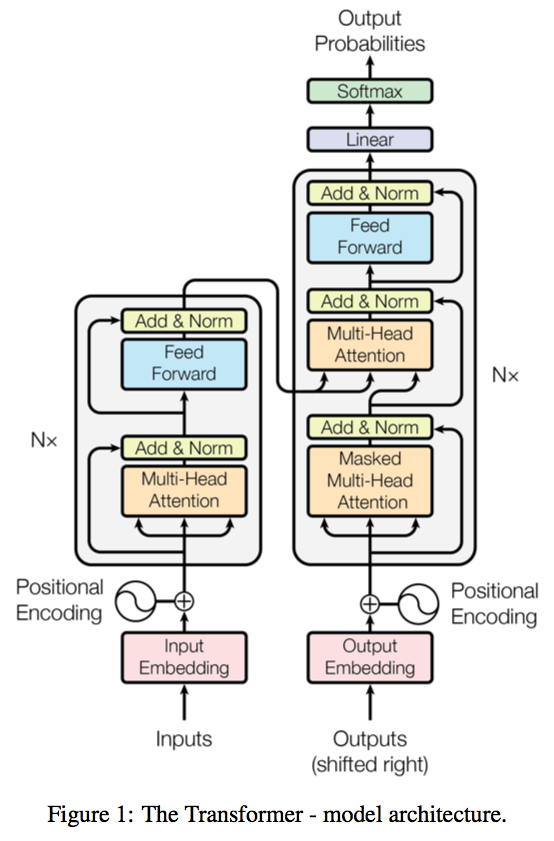
\includegraphics[width=0.35\linewidth,keepaspectratio]{transformer}
	\end{center}		

{\tiny (Ref: ``Attention is all you need''. 2017.  Aswani, Shazeer, Parmar, Uszkoreit,  Jones, Gomez, Kaiser, Polosukhin  https://arxiv.org/pdf/1706.03762.pdf}


			
\end{frame}

%%%%%%%%%%%%%%%%%%%%%%%%%%%%%%%%%%%%%%%%%%%%%%%%%%%%%%%%%%%
\begin{frame}[fragile]\frametitle{A High-Level Look}

Lets start with a very high-level view \ldots and then Zoom in each sub-blocks.

Here is the Transformer block and its i/o.

\begin{center}
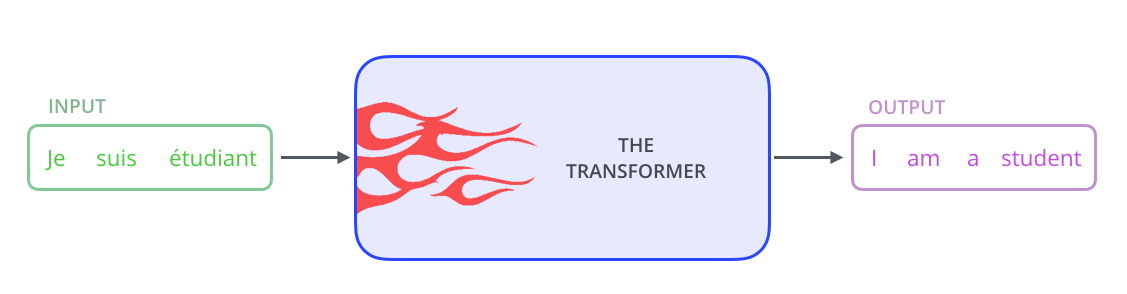
\includegraphics[width=0.8\linewidth,keepaspectratio]{transformer_jay}

{\tiny (Ref: ``The Illustrated Transformer'' - Jay Alammar)}
\end{center}		

\begin{itemize}
\item Main architecture: encoder-decoder ie sequence to sequence
\item Task: machine translation with parallel corpus (encoder-decoder)
\item Sub-tasks: Word Embedding (Encoder), Predict each translated word (Decoder)
\item can be done by RNNs, LSTMs, etc. But they had issues.
\item Here we bring parallelization.
\item Challenges? Different input-output sizes, different attention correspondence, word order matters, semantic preservation, compute cost, storage cost, etc.
\end{itemize}

			
\end{frame}

%%%%%%%%%%%%%%%%%%%%%%%%%%%%%%%%%%%%%%%%%%%%%%%%%%%%%%%%%%%
\begin{frame}[fragile]\frametitle{One level down}

Within Transformer block we have

\begin{center}
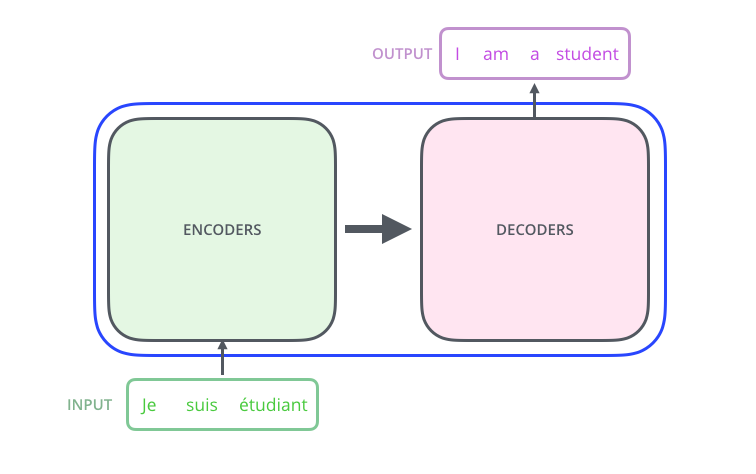
\includegraphics[width=0.6\linewidth,keepaspectratio]{transformer_encoders_decoders_jay}

{\tiny (Ref: ``The Illustrated Transformer'' - Jay Alammar)}
\end{center}		

Inference time flow: 
\begin{itemize}
\item Encoder takes input
\item Does some processing, creates a `latent` representation, sends it to decoder
\item Decoder processes this input to generate the output
\end{itemize}

What would be ML training flow?
			
\end{frame}

%%%%%%%%%%%%%%%%%%%%%%%%%%%%%%%%%%%%%%%%%%%%%%%%%%%%%%%%%%%
\begin{frame}[fragile]\frametitle{One level down}

Each sub-block ie Encoder-Decoder blocks are actually stacks of encoders decoders.

\begin{center}
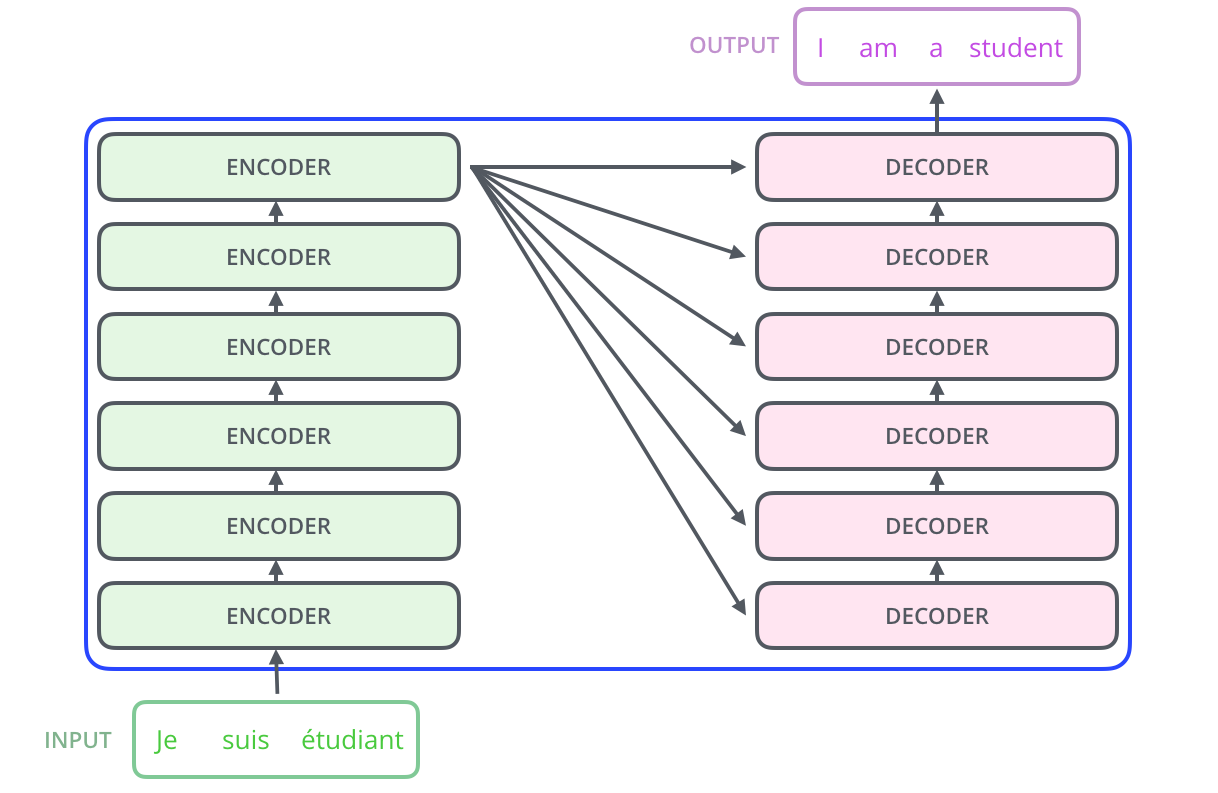
\includegraphics[width=0.6\linewidth,keepaspectratio]{transformer_encoder_decoder_stack_jay}

{\tiny (Ref: ``The Illustrated Transformer'' - Jay Alammar)}
\end{center}		

 
\begin{itemize}
\item Encoder has 6 blocks, so does Decoder. 
\item Why 6? Why not 7? They found it to be good. Like Hyper-parameter.
\end{itemize}

How many blocks GPT 3.5 has?
			
\end{frame}

%%%%%%%%%%%%%%%%%%%%%%%%%%%%%%%%%%%%%%%%%%%%%%%%%%%%%%%%%%%
\begin{frame}[fragile]\frametitle{One level down in Encoder Cell}

Each Encoder sub-block is actually stack of \ldots

\begin{columns}
    \begin{column}[T]{0.5\linewidth}
		\begin{center}
		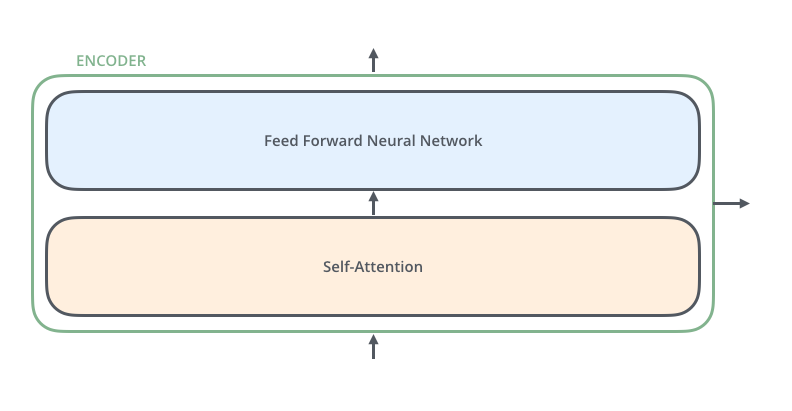
\includegraphics[width=\linewidth,keepaspectratio]{transformer_encoder_jay}
		
		{\tiny (Ref: ``The Illustrated Transformer'' - Jay Alammar)}
		\end{center}		
	\end{column}
	\begin{column}[T]{0.5\linewidth}
		\begin{itemize}
		\item Self Attention:  a layer that helps the encoder look at other words in the input sentence as it encodes a specific word.
		\item Feed Forward: The outputs of the self-attention layer are fed to a feed-forward neural network. The exact same feed-forward network is independently applied to each position.
		\end{itemize}
	\end{column}
\end{columns}
Input Embedding? Positional Embedding? Residual connections? batch normalization?
			
\end{frame}


%%%%%%%%%%%%%%%%%%%%%%%%%%%%%%%%%%%%%%%%%%%%%%%%%%%%%%%%%%%
\begin{frame}[fragile]\frametitle{Similarly on Decoder side}

Each Decoder sub-block is actually stack of \ldots


		\begin{center}
		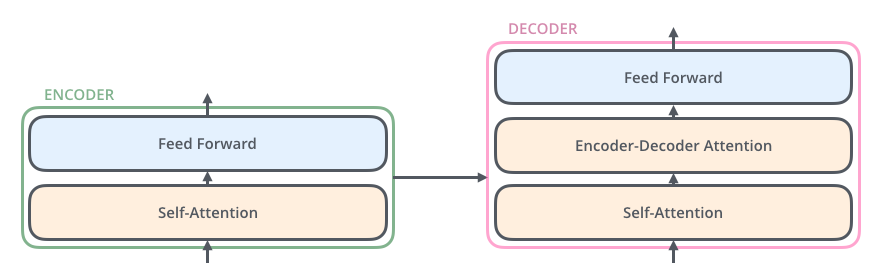
\includegraphics[width=\linewidth,keepaspectratio]{transformer_decoder_jay}
		
		{\tiny (Ref: ``The Illustrated Transformer'' - Jay Alammar)}

		\end{center}		
		

		\begin{itemize}
		\item The decoder also has both those layers (Self but Masked Attention and Feed Forward), but between them is an (cross) attention layer that helps the decoder focus on relevant parts of the input sentence
		\end{itemize}

		
\end{frame}

%%%%%%%%%%%%%%%%%%%%%%%%%%%%%%%%%%%%%%%%%%%%%%%%%%%%%%%%%%%
\begin{frame}[fragile]\frametitle{Transformer Encoder}

Actual architecture in the research paper.

\begin{columns}
    \begin{column}[T]{0.4\linewidth}
			\begin{center}
			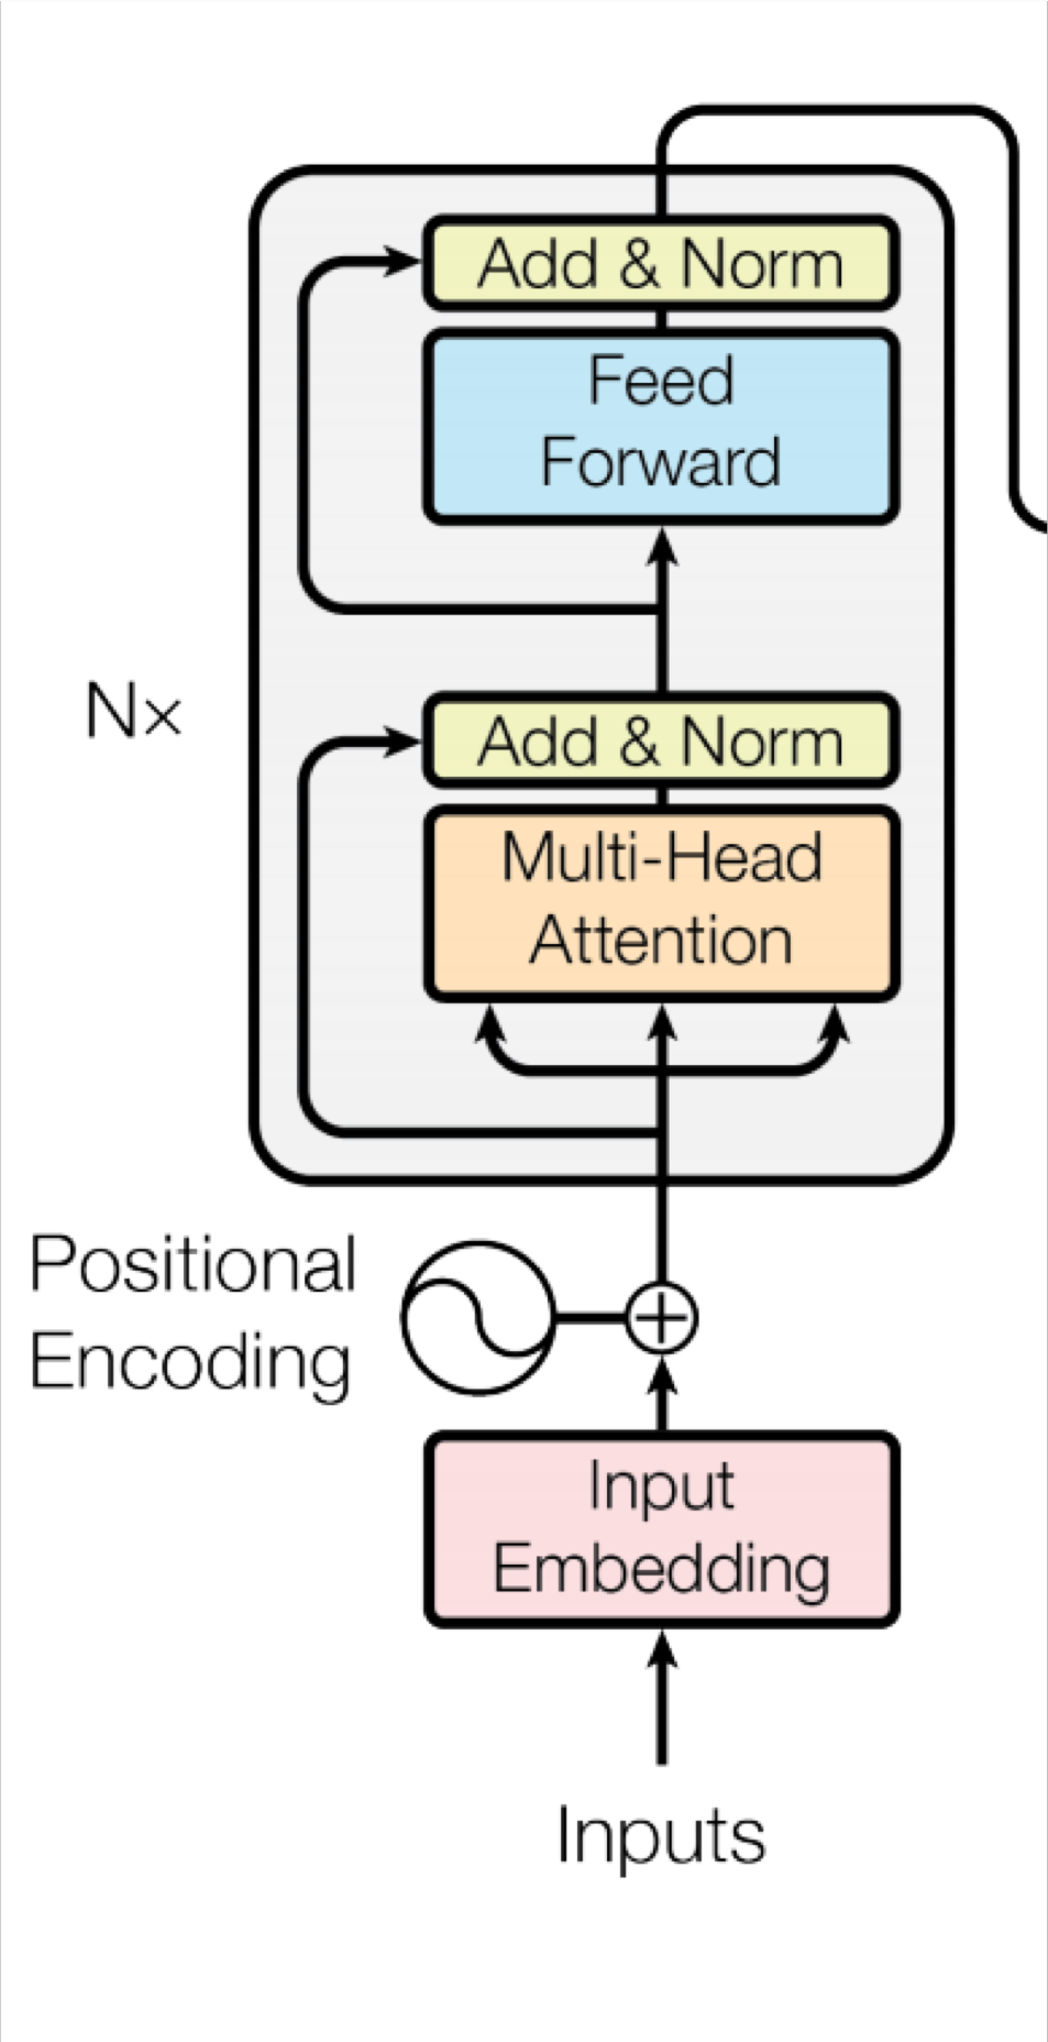
\includegraphics[width=0.6\linewidth,keepaspectratio]{bert70}
			\end{center}		
		\end{column}
    \begin{column}[T]{0.6\linewidth}
      \begin{itemize}
			\item For encoder block, initial input, tokenization, embedding, positional encoding, happens at the start, then the first Encoder cell starts.
			\item In each cell, we have multi-head self attention, residual connections, batch normalization and then feed forward then again residual + batch normalization.
			\item Output of this cell is passed to the next encoder cell.
			\item Output of the last encoder cell in the encoder block is passed to the Decoder block.
			\end{itemize}
    \end{column}
  \end{columns}
		
     \begin{itemize}
			\item Mind well, that each word here gets processed parallelly, unlike RNN or LSTM.
			\item Cells are repeated 6 times (in vertical stack)
			\end{itemize}		
\end{frame}

%%%%%%%%%%%%%%%%%%%%%%%%%%%%%%%%%%%%%%%%%%%%%%%%%%%%%%%%%%%
\begin{frame}[fragile]\frametitle{Transformer Decoder}


			\begin{center}
			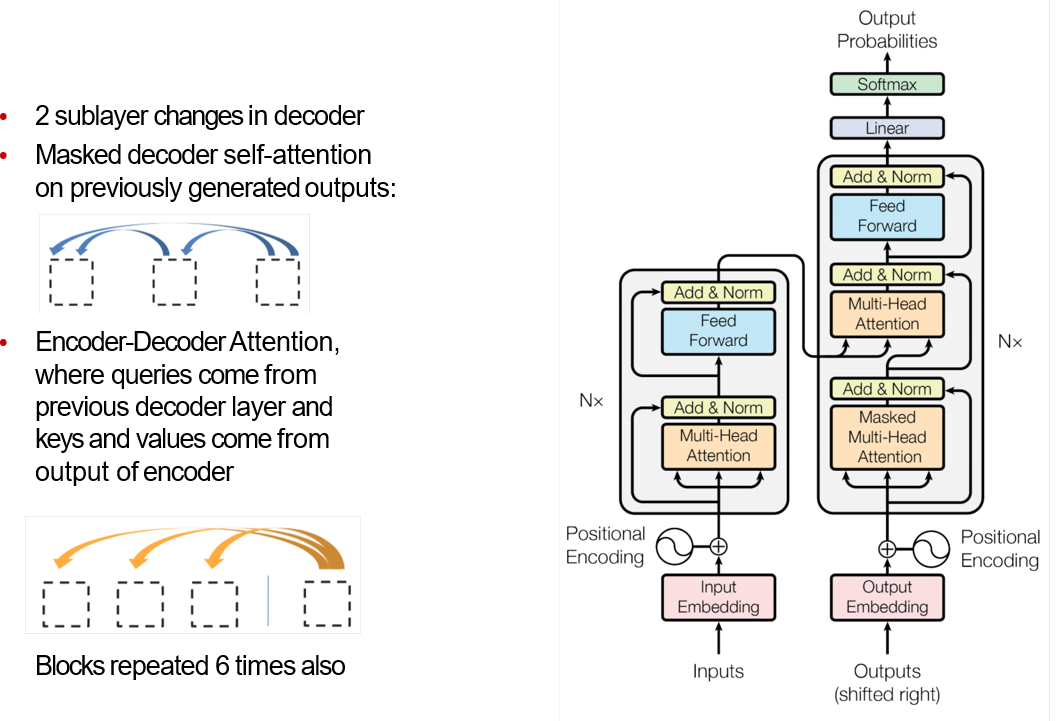
\includegraphics[width=\linewidth,keepaspectratio]{bert71}
			\end{center}		

			
\end{frame}

%%%%%%%%%%%%%%%%%%%%%%%%%%%%%%%%%%%%%%%%%%%%%%%%%%%%%%%%%%%
\begin{frame}[fragile]\frametitle{Transformer Encoder-Decoder}

			\begin{center}
			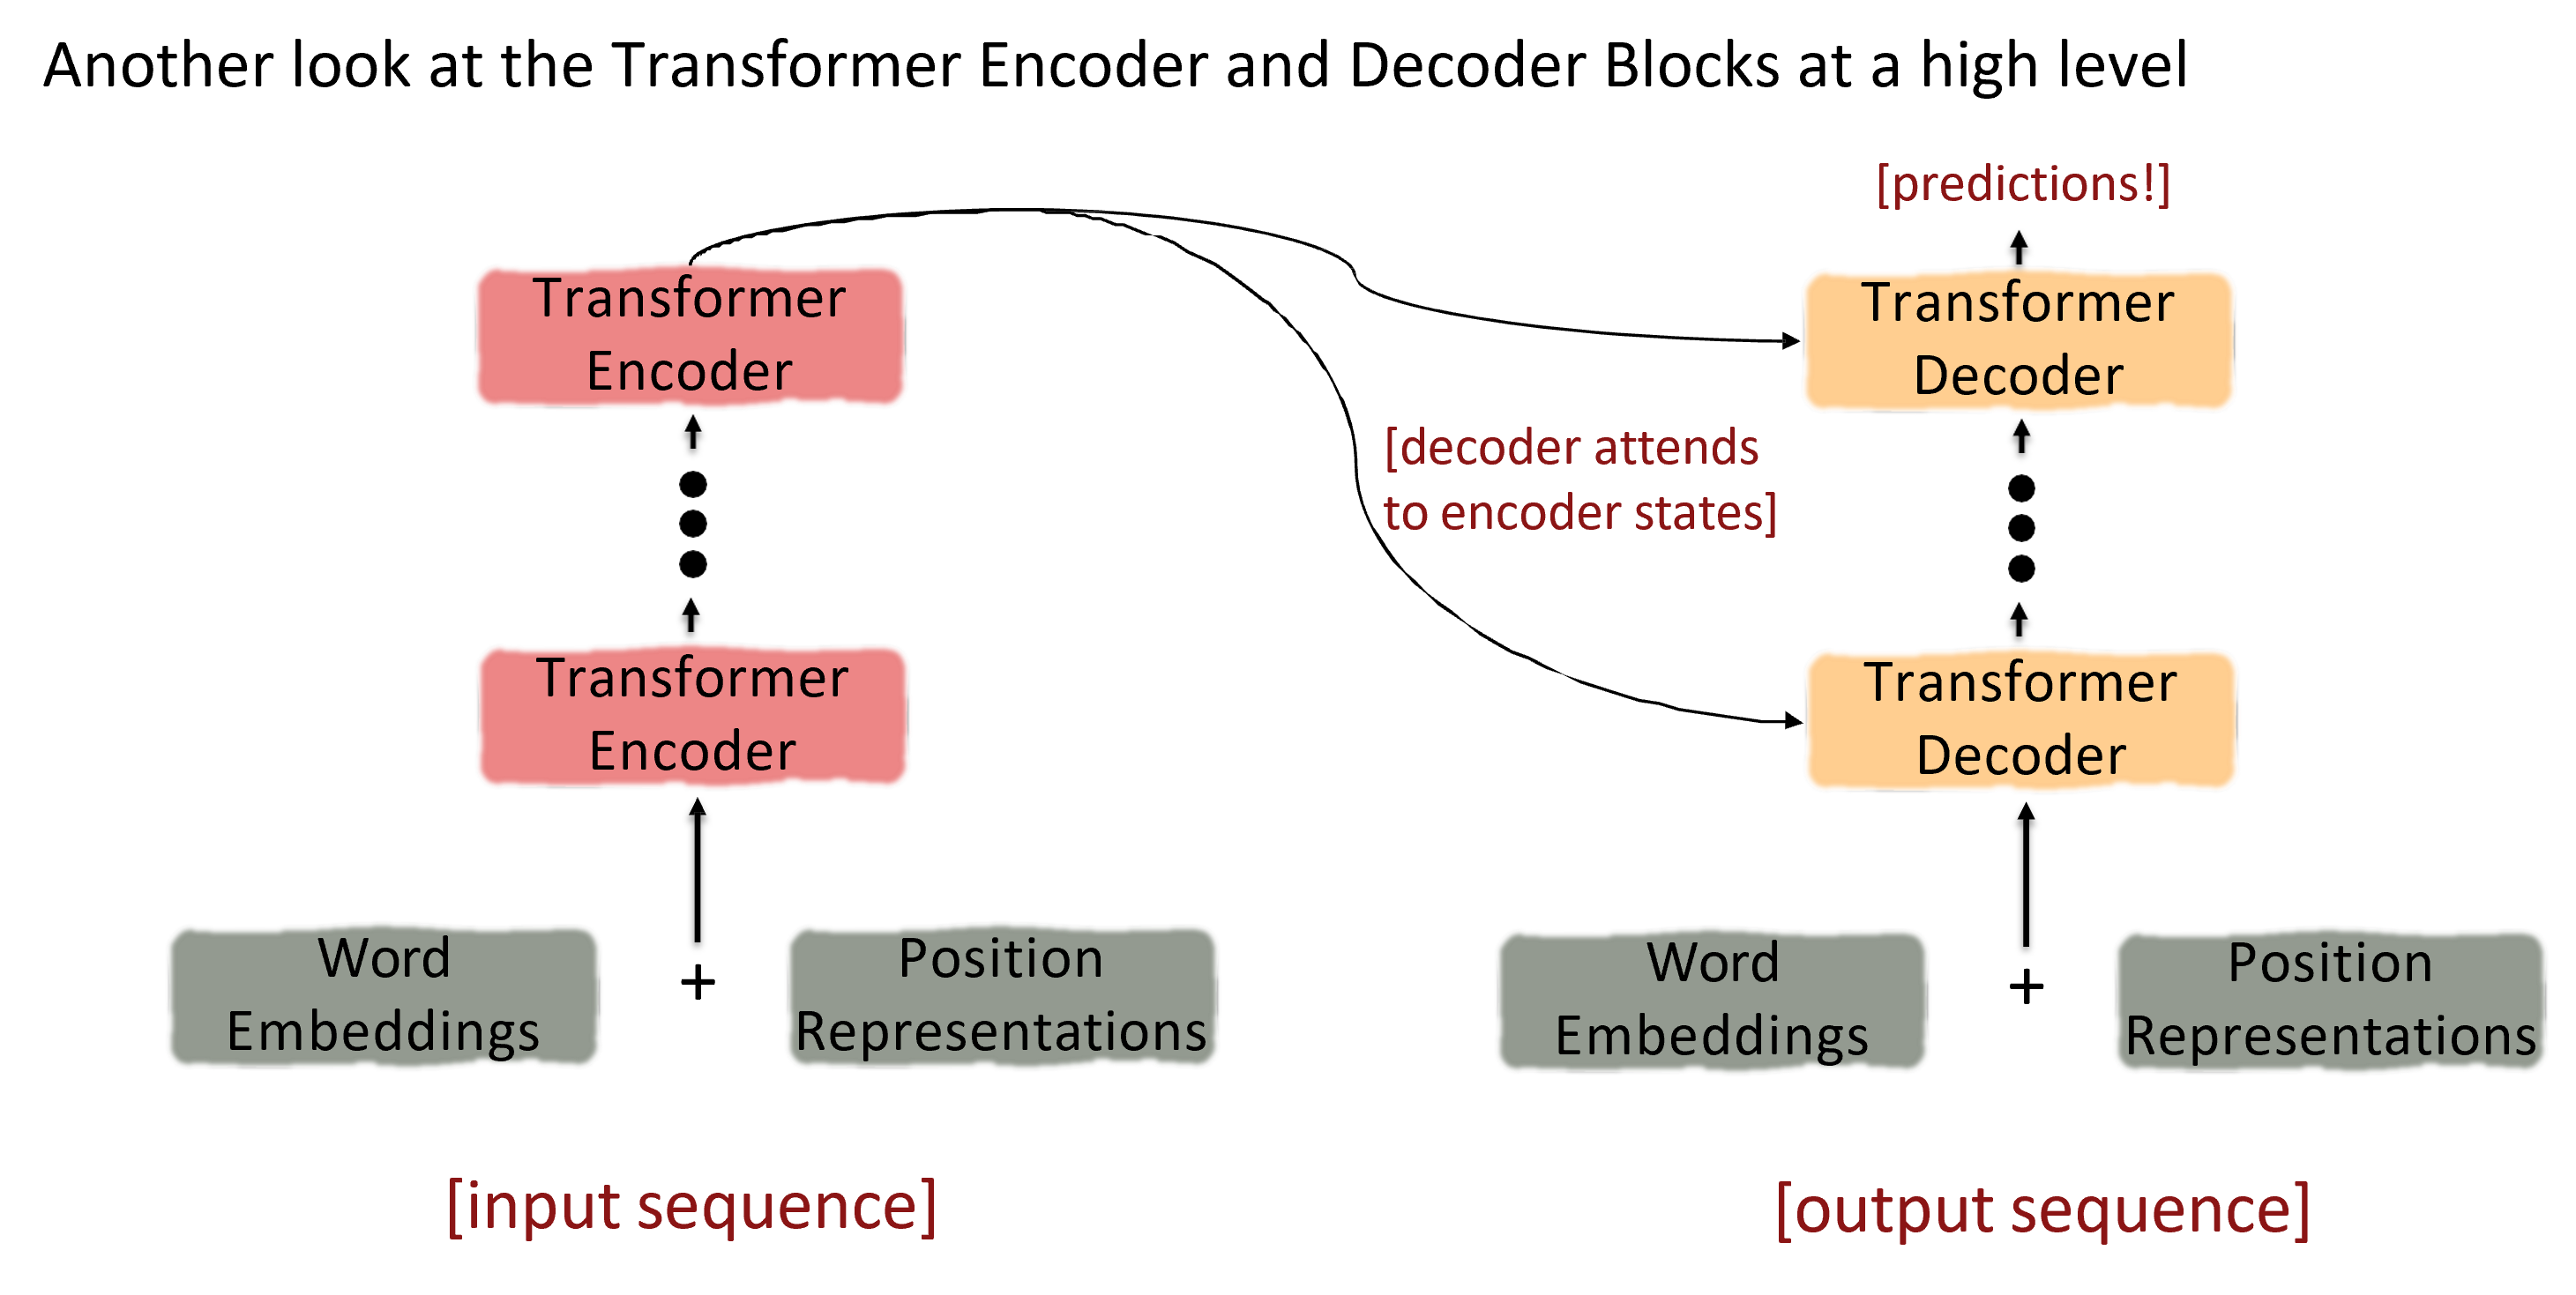
\includegraphics[width=\linewidth,keepaspectratio]{bert72}
			\end{center}		

			
\end{frame}

%%%%%%%%%%%%%%%%%%%%%%%%%%%%%%%%%%%%%%%%%%%%%%%%%%%%%%%%%%%
\begin{frame}[fragile]\frametitle{Transformer Encoder-Decoder}
Next, let’s look at the Transformer Encoder and Decoder Blocks in action


      \begin{itemize}
			\item Imagine Machine Translation: French to English
			\item What would be ML training flow?
			\item What would be ML inference flow?
			\item Can we use input or output text as is, ie in string format?
			\item Whats the NLP way of making text available for ML or DL algorithms?
	\end{itemize}
			
\end{frame}

%%%%%%%%%%%%%%%%%%%%%%%%%%%%%%%%%%%%%%%%%%%%%%%%%%%%%%%%%%%%%%%%%%%%%%%%%%%%%%%%%%
\begin{frame}[fragile]\frametitle{}
\begin{center}
{\Large Block: Input Embedding}
\end{center}
\end{frame}

%%%%%%%%%%%%%%%%%%%%%%%%%%%%%%%%%%%%%%%%%%%%%%%%%%%%%%%%%%%
\begin{frame}[fragile]\frametitle{Convert Word to Vectors}


\begin{center}
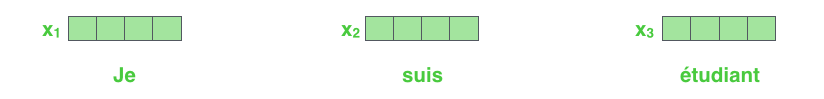
\includegraphics[width=\linewidth,keepaspectratio]{embeddings_jay}


{\tiny (Ref: ``The Illustrated Transformer'' - Jay Alammar)}
\end{center}		


\begin{itemize}
\item Either by Frequency based ie one-hot or tf-idf or Neural way ie Word2Vec (in paper)
\item Or put embedding layer (like in TensorFlow or Keras NLP, which also gets trained)
\item Size: 512, a hyper-parameter we can set – basically it would be the length of the longest sentence in our training dataset.
\item After embedding the words in our input sequence, each of them flows through each of the two layers of the encoder.
\end{itemize}

\end{frame}

%%%%%%%%%%%%%%%%%%%%%%%%%%%%%%%%%%%%%%%%%%%%%%%%%%%%%%%%%%%
\begin{frame}[fragile]\frametitle{Flow of Vectors in Encoder Cell}


\begin{columns}
    \begin{column}[T]{0.5\linewidth}
\begin{center}
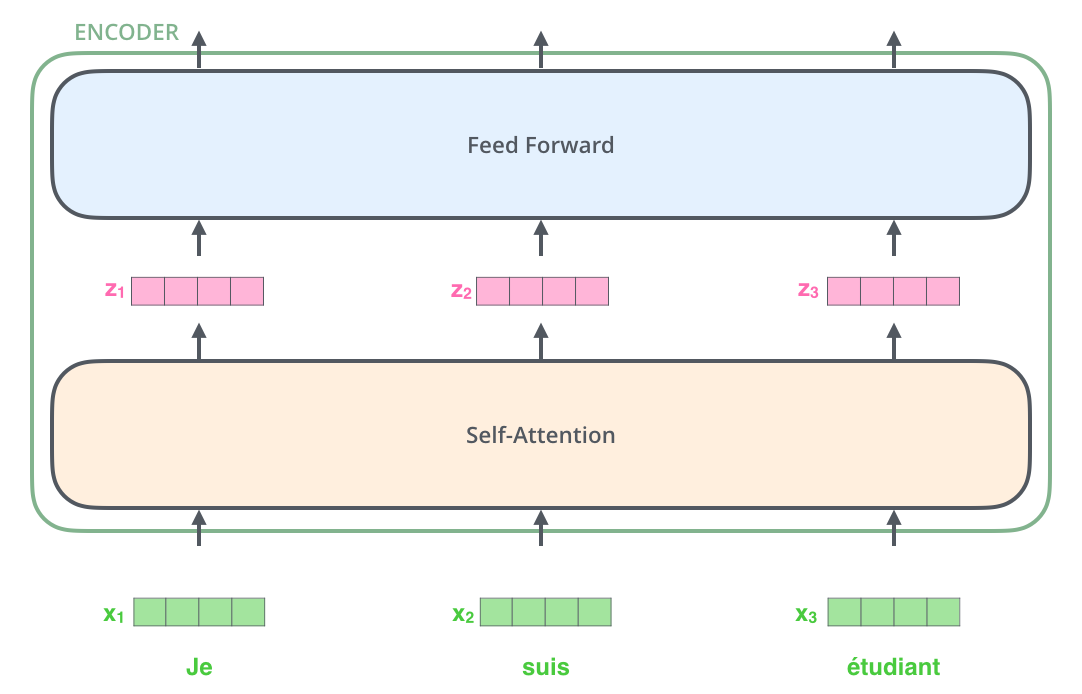
\includegraphics[width=\linewidth,keepaspectratio]{encoder_with_tensors_jay}


{\tiny (Ref: ``The Illustrated Transformer'' - Jay Alammar)}
\end{center}		

		\end{column}
    \begin{column}[T]{0.5\linewidth}
\begin{itemize}
\item Key property : the word in each position flows through its own path in the encoder. 
\item Calculations in the self-attention layer do need other words. 
\item But later, in the feed-forward layer does not have those dependencies, \item thus the various paths can be executed in parallel while flowing through the feed-forward layer.
\end{itemize}
    \end{column}
  \end{columns}
\end{frame}

%%%%%%%%%%%%%%%%%%%%%%%%%%%%%%%%%%%%%%%%%%%%%%%%%%%%%%%%%%%
\begin{frame}[fragile]\frametitle{Flow of Vectors in Encoder Block}


\begin{center}
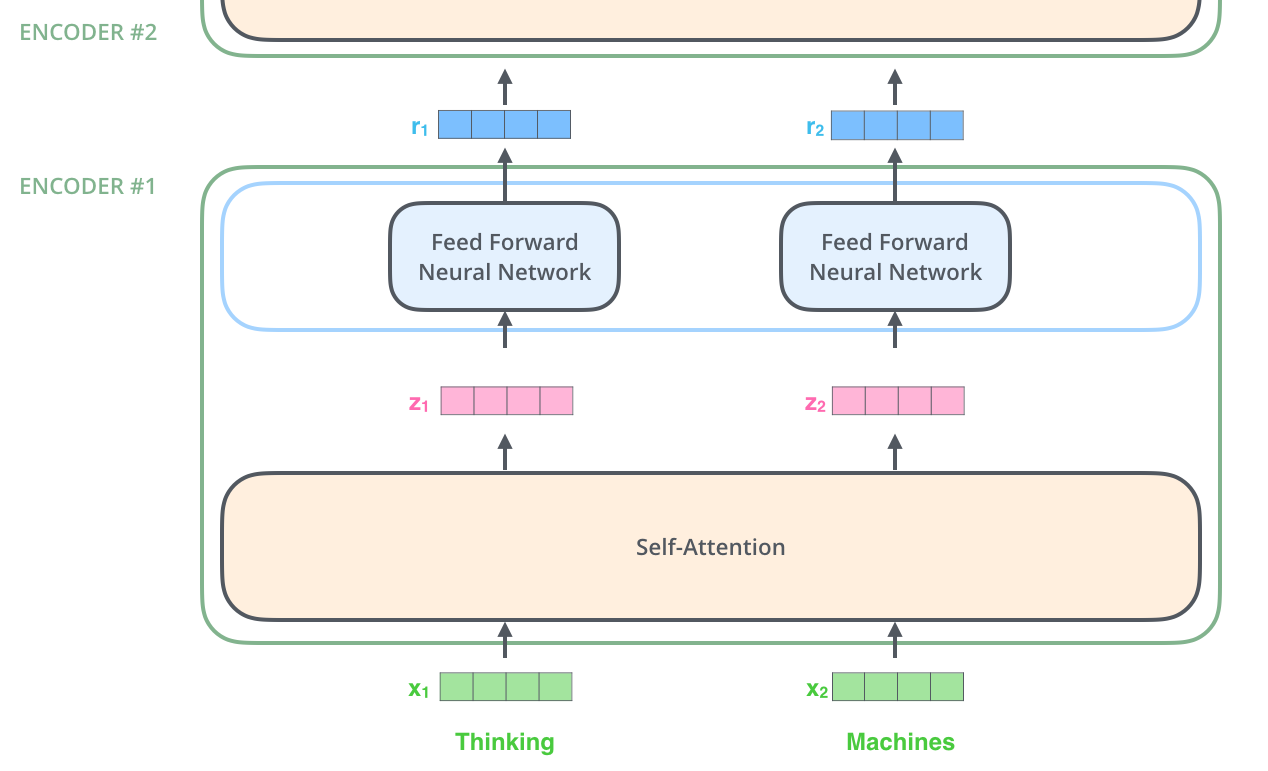
\includegraphics[width=0.6\linewidth,keepaspectratio]{encoder_with_tensors_block_jay}


{\tiny (Ref: ``The Illustrated Transformer'' - Jay Alammar)}
\end{center}		


\begin{itemize}
\item The word at each position passes through a self-attention process. 
\item Then, they each pass through a feed-forward neural network -- the exact same network with each vector flowing through it separately.
\item Meaning ALL weights in these cells, block are same for ALL words going through in each epoch, of course they get adjusted during back propagation.
\end{itemize}

\end{frame}


%%%%%%%%%%%%%%%%%%%%%%%%%%%%%%%%%%%%%%%%%%%%%%%%%%%%%%%%%%%%%%%%%%%%%%%%%%%%%%%%%%
\begin{frame}[fragile]\frametitle{}
\begin{center}
{\Large Block: Positional Encoding}
\end{center}
\end{frame}

%%%%%%%%%%%%%%%%%%%%%%%%%%%%%%%%%%%%%%%%%%%%%%%%%%%%%%%%%%%
\begin{frame}[fragile]\frametitle{Why?}


\begin{itemize}
\item In languages like English (unlike Sanskrit) word order matters, meaning 'Suresh ate chicken' and 'chicken ate Suresh' are two different things.
\item As input is all word vectors together, parallel, (unlike RNN or LSTM where they are sequential ie one after another, there the order is preserved), the sense of position is lost.
\item Need to add that information by unique position value/signature.
\item A cool mechanism (similar to Fourier Transform) was employed.
\end{itemize}

\end{frame}

%%%%%%%%%%%%%%%%%%%%%%%%%%%%%%%%%%%%%%%%%%%%%%%%%%%%%%%%%%%
\begin{frame}[fragile]\frametitle{Representing The Order of The Sequence Using Positional Encoding}


\begin{columns}
    \begin{column}[T]{0.5\linewidth}
\begin{center}
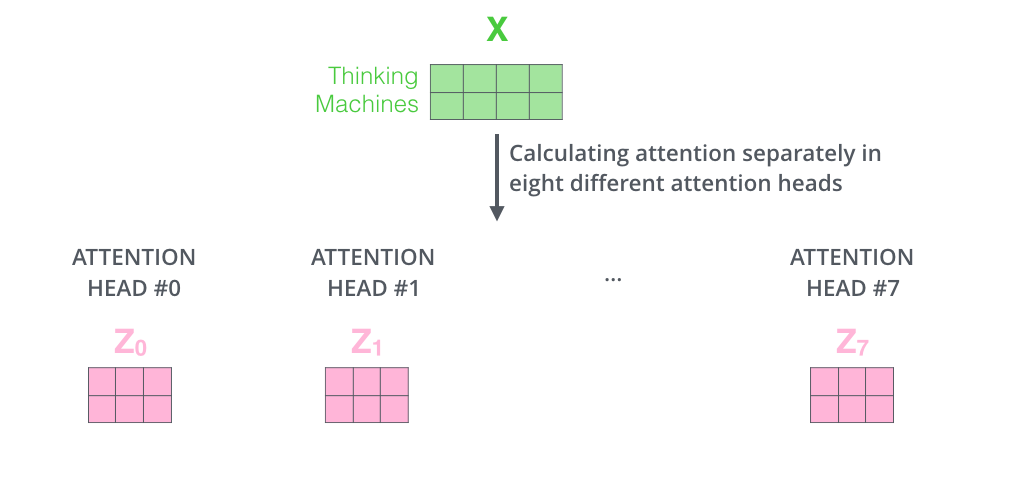
\includegraphics[width=\linewidth,keepaspectratio]{transformer_attention_heads_z_jay}


{\tiny (Ref: ``The Illustrated Transformer'' - Jay Alammar)}
\end{center}		

		\end{column}
    \begin{column}[T]{0.5\linewidth}

\begin{itemize}
\item In languages like English (unlike Sanskrit) word order matters, meaning 'Suresh ate chicken' and 'chicken ate Suresh' are two different things.
\item As input is all word vectors together, parallel, (unlike RNN or LSTM where they are sequential ie one after another, there the order is preserved), the sense of position is lost.
\item Need to add that information by unique position value/signature.
\item A cool mechanism (similar to Fourier Transform) was employed.
\end{itemize}
    \end{column}
  \end{columns}
\end{frame}

%%%%%%%%%%%%%%%%%%%%%%%%%%%%%%%%%%%%%%%%%%%%%%%%%%%%%%%%%%%%%%%%%%%%%%%%%%%%%%%%%%
\begin{frame}[fragile]\frametitle{}
\begin{center}
{\Large Self Attention}
\end{center}
\end{frame}

%%%%%%%%%%%%%%%%%%%%%%%%%%%%%%%%%%%%%%%%%%%%%%%%%%%%%%%%%%%
\begin{frame}[fragile]\frametitle{Self-Attention at a High Level}

\begin{columns}
    \begin{column}[T]{0.5\linewidth}
\begin{center}
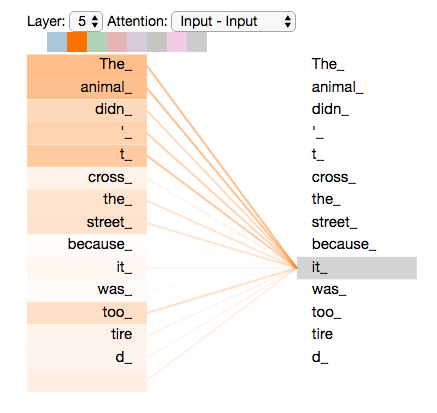
\includegraphics[width=\linewidth,keepaspectratio]{transformer_self-attention_visualization_jay}


{\tiny (Ref: ``The Illustrated Transformer'' - Jay Alammar)}
\end{center}		

		\end{column}
    \begin{column}[T]{0.5\linewidth}

\begin{itemize}
\item ``The animal didn't cross the street because it was too tired'', what ``it'' refers to?
\item  the street or to the animal?
\item For “it”, self-attention mechanism (some how, or should) allows it to associate “it” with “animal”.
\item ie for each word (each position in the input sequence), self attention allows it to look at other positions in the input sequence for clues that can help lead to a better encoding for this word.
\item Lets see how that can be achieved.
\end{itemize}
    \end{column}
  \end{columns}
\end{frame}

%%%%%%%%%%%%%%%%%%%%%%%%%%%%%%%%%%%%%%%%%%%%%%%%%%%%%%%%%%%
\begin{frame}[fragile]\frametitle{Self-Attention in Principle}


\begin{itemize}
\item Slight digression: lets say you have database of key($k$)-value($v$) pairs, then you have a query ($q$), which needs to go and search in the database and get corresponding or closest value.
\item So, $q$ is matched (similarity) with all $k$s, whichever matches most, its $v$ is returned.
\item Same mechanism is used to create self-attention score.
\item For each word-vector in the sentence ($q$), we find similarity with $k$ vectors or all the words, which ever matches most, its $v$ vector is returned.
\end{itemize}

\end{frame}

%%%%%%%%%%%%%%%%%%%%%%%%%%%%%%%%%%%%%%%%%%%%%%%%%%%%%%%%%%%
\begin{frame}[fragile]\frametitle{Self-Attention in Detail}

\begin{columns}
    \begin{column}[T]{0.5\linewidth}
\begin{center}
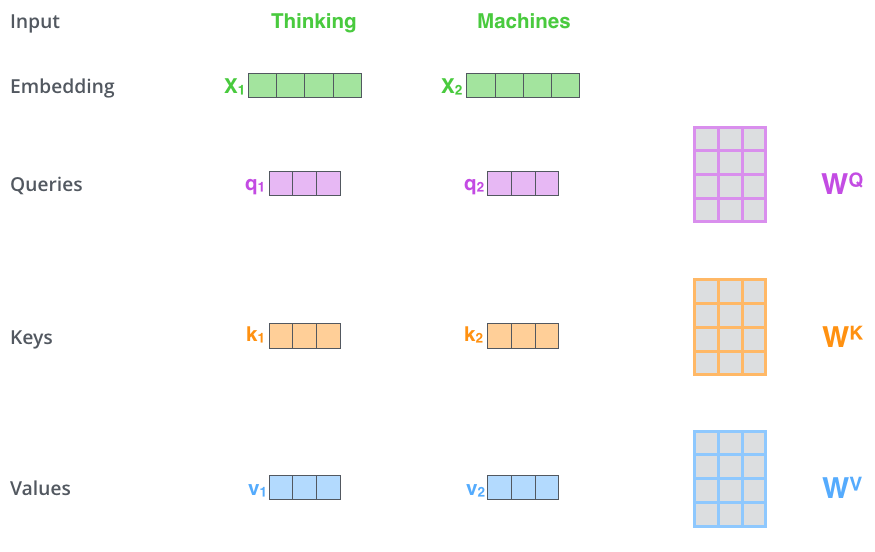
\includegraphics[width=\linewidth,keepaspectratio]{transformer_self_attention_vectors_jay}


{\tiny (Ref: ``The Illustrated Transformer'' - Jay Alammar)}
\end{center}		

		\end{column}
    \begin{column}[T]{0.5\linewidth}

\begin{itemize}
\item Create three vectors from each of the encoder’s input vectors (in this case, the embedding of each word). 
\item So for each word, we create a Query vector, a Key vector, and a Value vector. \item These vectors are created by multiplying the embedding by three matrices, which are trained during the training process.
\end{itemize}
    \end{column}
  \end{columns}
  
  Multiplying $x_1$ by the $W^Q$ weight matrix produces $q_1$, the ``query`` vector associated with that word. We end up creating a ``query'', a ``key'', and a ``value'' projection of each word in the input sentence.
  
  Note: new vectors are smaller, 64, while the embedding and encoder input/output vectors have dimensionality of 512. They don’t HAVE to be smaller, just a choice.
\end{frame}

%%%%%%%%%%%%%%%%%%%%%%%%%%%%%%%%%%%%%%%%%%%%%%%%%%%%%%%%%%%
\begin{frame}[fragile]\frametitle{Self-Attention Scores}

\begin{columns}
    \begin{column}[T]{0.5\linewidth}
\begin{center}
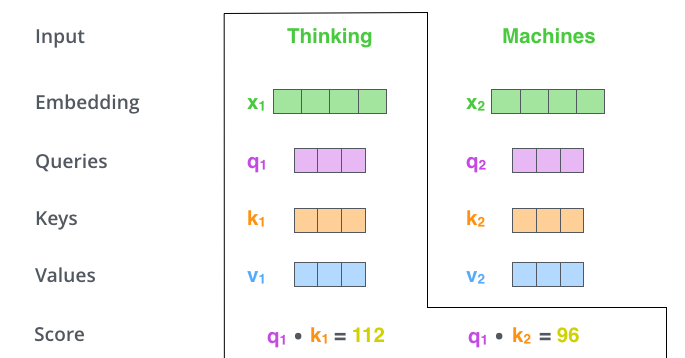
\includegraphics[width=\linewidth,keepaspectratio]{transformer_self_attention_score_jay}


{\tiny (Ref: ``The Illustrated Transformer'' - Jay Alammar)}
\end{center}		

		\end{column}
    \begin{column}[T]{0.5\linewidth}

\begin{itemize}
\item Calculating the self-attention for the first word in this example, “Thinking”. 
\item Need to score each word of the input sentence against this word, thats its importance wrt that word
\item score = dot product of words query vector with key vector of the running words. Each is a single scalar value. So, score for first word $w_1 = q_1 k_1 + q_1 k_2 + \ldots$
\end{itemize}
    \end{column}
  \end{columns}

* Please note that in the diagram the Embedding vectors also include positional encoding incorporated inside.
\end{frame}

%%%%%%%%%%%%%%%%%%%%%%%%%%%%%%%%%%%%%%%%%%%%%%%%%%%%%%%%%%%
\begin{frame}[fragile]\frametitle{Self-Attention Scores}

\begin{columns}
    \begin{column}[T]{0.5\linewidth}
\begin{center}
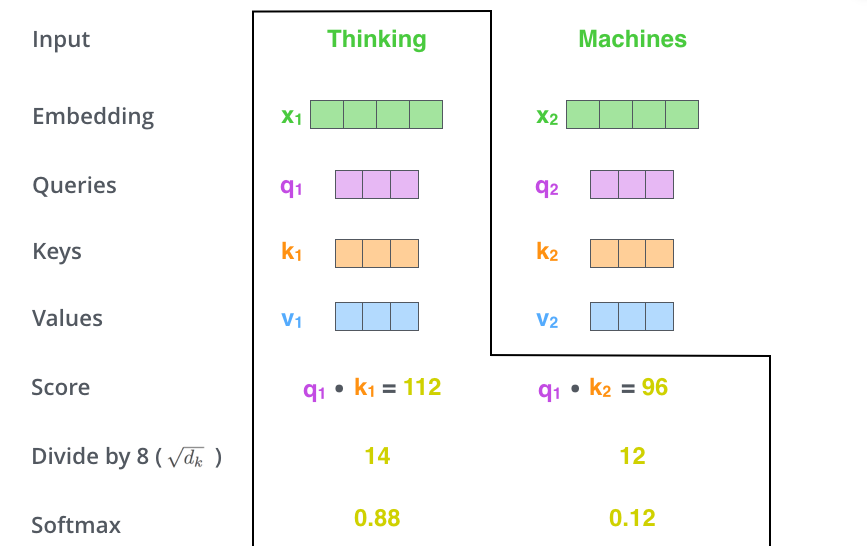
\includegraphics[width=\linewidth,keepaspectratio]{self-attention_softmax_jay}


{\tiny (Ref: ``The Illustrated Transformer'' - Jay Alammar)}
\end{center}		

		\end{column}
    \begin{column}[T]{0.5\linewidth}

\begin{itemize}
\item Divide the scores by 8 (the square root of the dimension of the key vectors used in the paper – 64. 
\item This leads to having more stable gradients. There could be other possible values here, but this is the default), 
\item then pass the result through a softmax that normalizes from 0 to 1

\end{itemize}
    \end{column}
  \end{columns}
  
   Note: Clearly word with itself will have the highest softmax score, thats ok
 but then next matching-high scores have importance

* Please note that in the diagram the Embedding vectors also include positional encoding incorporated inside.
\end{frame}

%%%%%%%%%%%%%%%%%%%%%%%%%%%%%%%%%%%%%%%%%%%%%%%%%%%%%%%%%%%
\begin{frame}[fragile]\frametitle{Self-Attention Scores with Value Vectors}

\begin{columns}
    \begin{column}[T]{0.5\linewidth}
\begin{center}
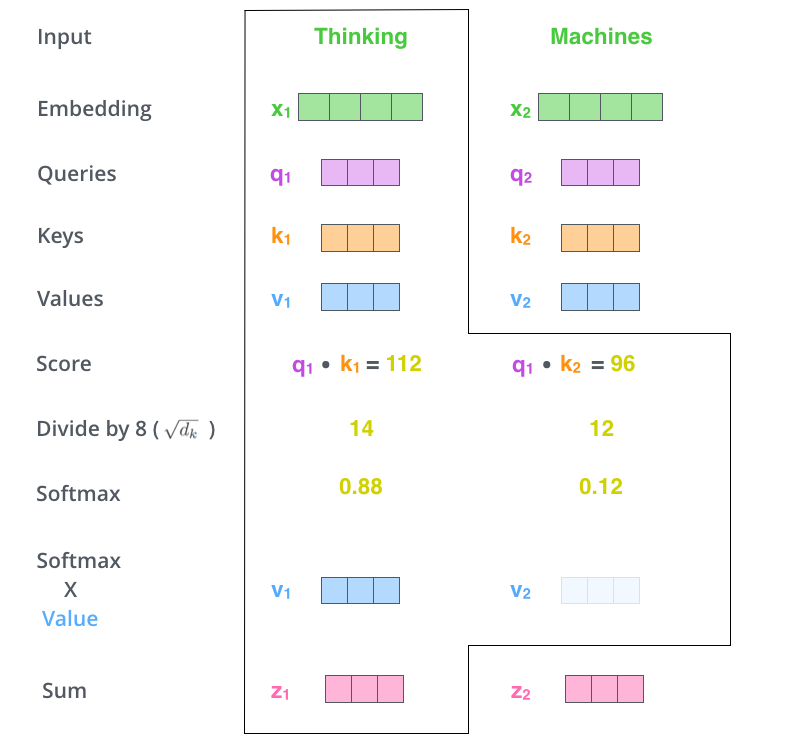
\includegraphics[width=\linewidth,keepaspectratio]{self-attention-output_jay}


{\tiny (Ref: ``The Illustrated Transformer'' - Jay Alammar)}
\end{center}		

		\end{column}
    \begin{column}[T]{0.5\linewidth}

\begin{itemize}
\item Multiply each value vector by the softmax scores respectively
\item The intuition here is to keep intact the values of the word(s) we want to focus on, and drown-out irrelevant words, basically weighted per position.
\item The last step is to sum up the weighted value vectors.
\item This produces the output of the self-attention layer at this position (for the first word).
\end{itemize}
    \end{column}
  \end{columns}

* Please note that in the diagram the Embedding vectors also include positional encoding incorporated inside.
\end{frame}

%%%%%%%%%%%%%%%%%%%%%%%%%%%%%%%%%%%%%%%%%%%%%%%%%%%%%%%%%%%
\begin{frame}[fragile]\frametitle{Self-Attention Scores in a Matrix Way}

\begin{columns}
    \begin{column}[T]{0.5\linewidth}
\begin{center}
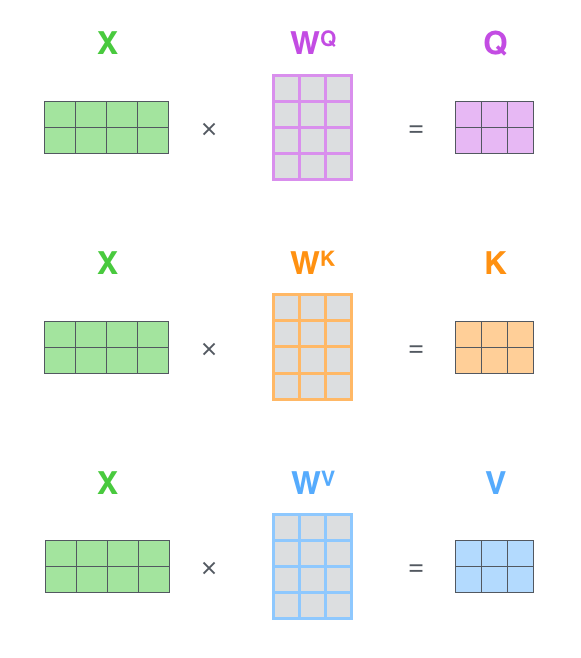
\includegraphics[width=0.8\linewidth,keepaspectratio]{self-attention-matrix-calculation_jay}


{\tiny (Ref: ``The Illustrated Transformer'' - Jay Alammar)}
\end{center}		

		\end{column}
    \begin{column}[T]{0.5\linewidth}

\begin{itemize}
\item Assuming two words in the sentence, so number of rows are two, num columns are 512 (but shown 4 just for brevity) and the q/k/v vectors (64, or 3 boxes in the figure)
\item  Calculate the Query, Key, and Value matrices. 
\item Input sentence vector is matrix $X$, and multiplying it by the weight matrices to be trained ($W^Q, W^K, W^V$).
\end{itemize}
    \end{column}
  \end{columns}

* Please note that in the diagram the Embedding vectors $X$ also include positional encoding incorporated inside.
\end{frame}

%%%%%%%%%%%%%%%%%%%%%%%%%%%%%%%%%%%%%%%%%%%%%%%%%%%%%%%%%%%
\begin{frame}[fragile]\frametitle{Self-Attention Scores in a single formula}


\begin{center}
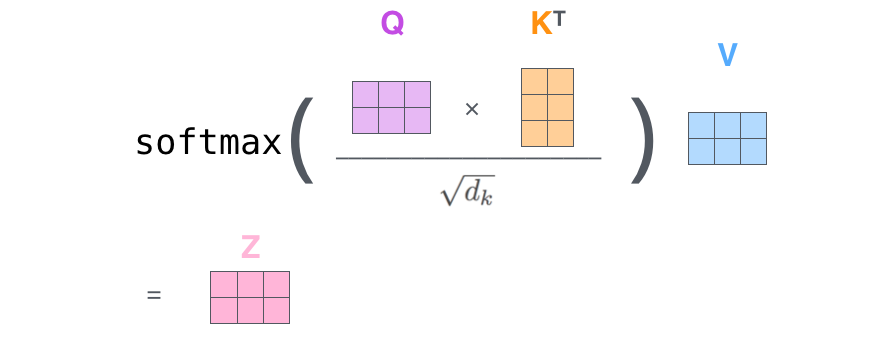
\includegraphics[width=\linewidth,keepaspectratio]{self-attention-matrix-calculation-2_jay}


{\tiny (Ref: ``The Illustrated Transformer'' - Jay Alammar)}
\end{center}		

\end{frame}




% %%%%%%%%%%%%%%%%%%%%%%%%%%%%%%%%%%%%%%%%%%%%%%%%%%%%%%%%%%%
% \begin{frame}[fragile]\frametitle{Dot-Product Attention}


      % \begin{itemize}
			% \item Inputs: a query q and a set of key-value (k-v) pairs to an output
			% \item Query, keys, values, and output are all vectors
			% \item Output is weighted sum of values, where
			% \item Weight of each value is computed by an inner product of query and corresponding key
			% \item Queries and keys have same dimensionality $d_k$ , value have $d_v$
			% \end{itemize}
			
			% \begin{center}
			% 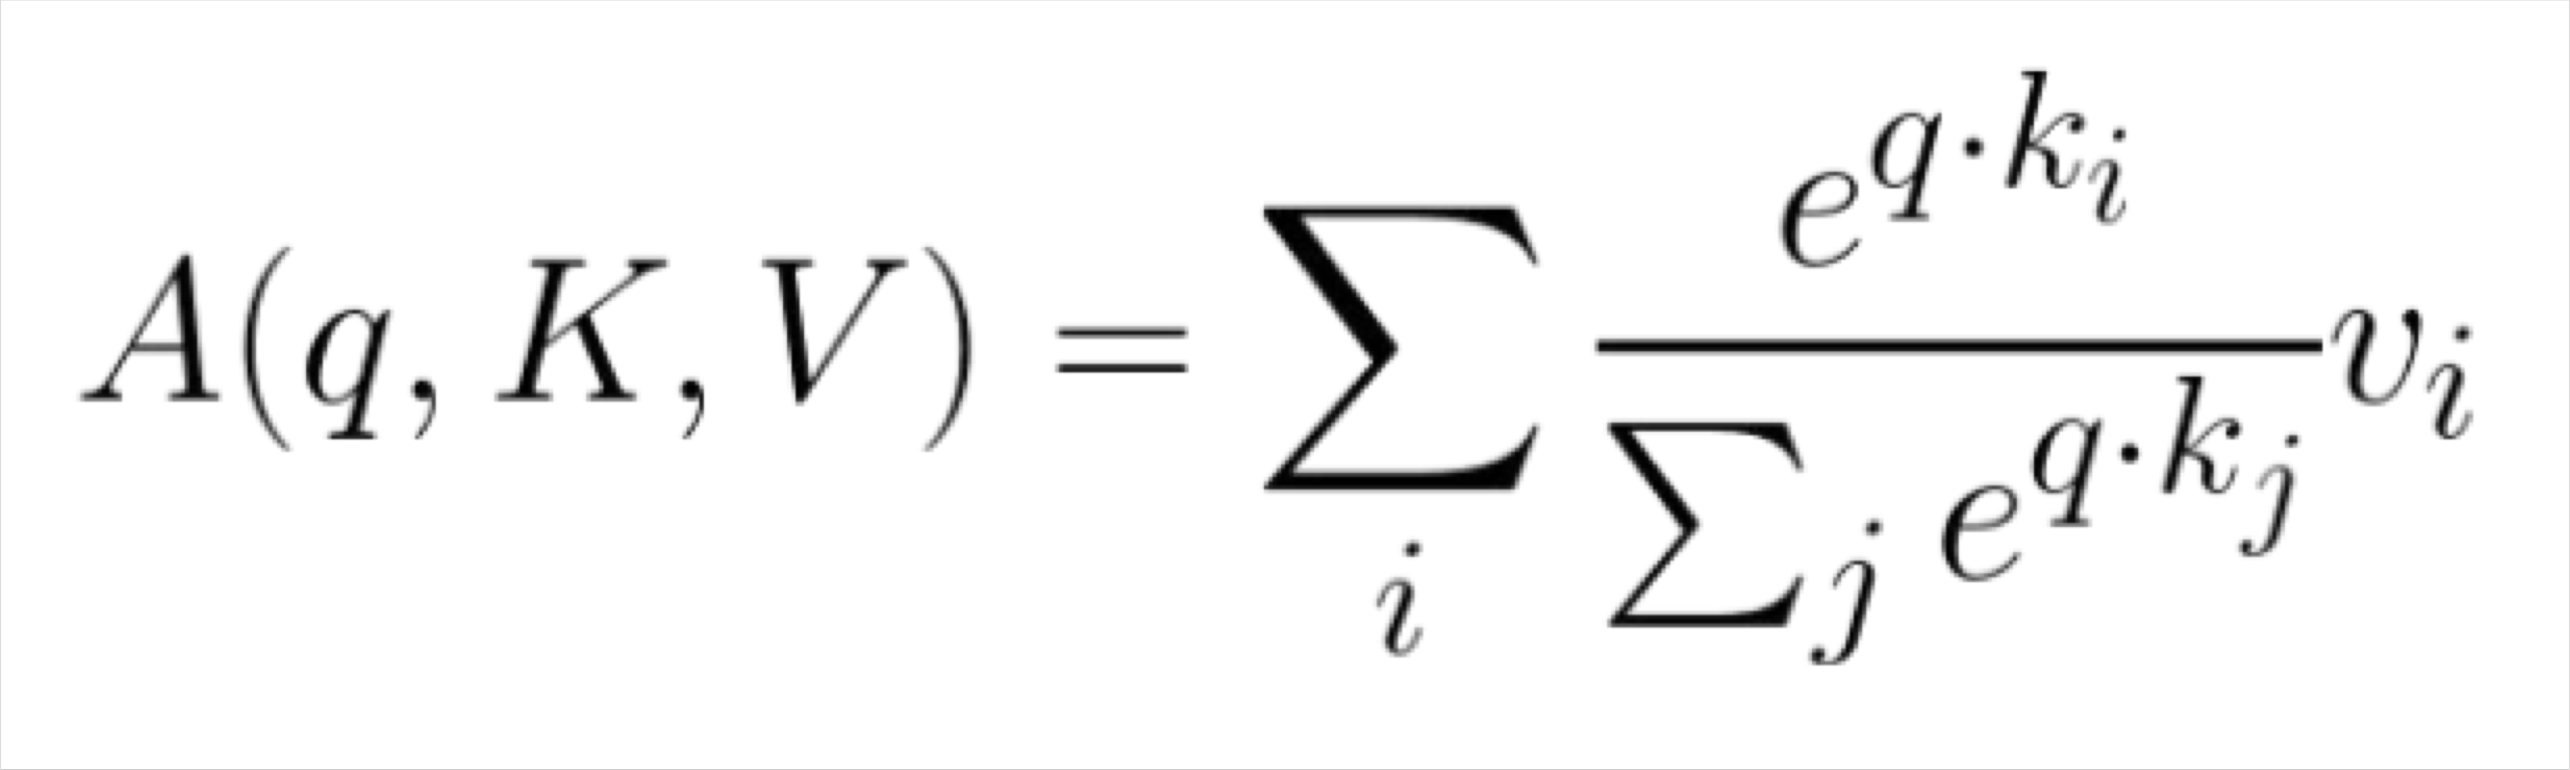
\includegraphics[width=0.4\linewidth,keepaspectratio]{bert73}
			% \end{center}		
			
			% % {\tiny (Ref: CS224n: Natural Language Processing with Deep Learning - Christopher Manning)}

% \end{frame}

% %%%%%%%%%%%%%%%%%%%%%%%%%%%%%%%%%%%%%%%%%%%%%%%%%%%%%%%%%%%
% \begin{frame}[fragile]\frametitle{Matrix notation}


      % \begin{itemize}
			% \item Inputs: a query q and a set of key-value (k-v) pairs to an output
			% \item Query, keys, values, and output are all vectors
			% \item Output is weighted sum of values, where
			% \item Weight of each value is computed by an inner product of query and corresponding key
			% \item Queries and keys have same dimensionality $d_k$ , value have $d_v$
			% \end{itemize}
			
			% \begin{center}
			% 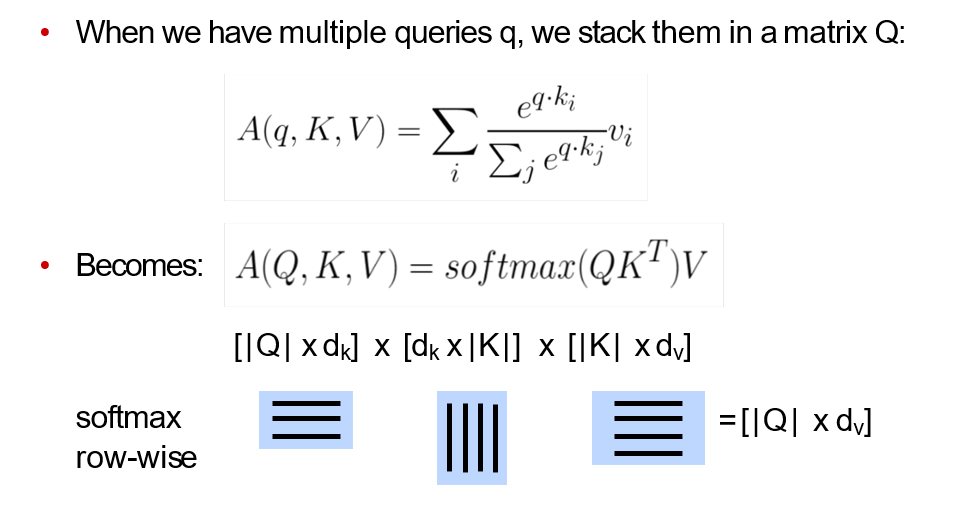
\includegraphics[width=0.8\linewidth,keepaspectratio]{bert74}
			% \end{center}		
			
			% % {\tiny (Ref: CS224n: Natural Language Processing with Deep Learning - Christopher Manning)}

% \end{frame}

% %%%%%%%%%%%%%%%%%%%%%%%%%%%%%%%%%%%%%%%%%%%%%%%%%%%%%%%%%%%
% \begin{frame}[fragile]\frametitle{Key-Query-Value Attention}

			
			% \begin{center}
			% 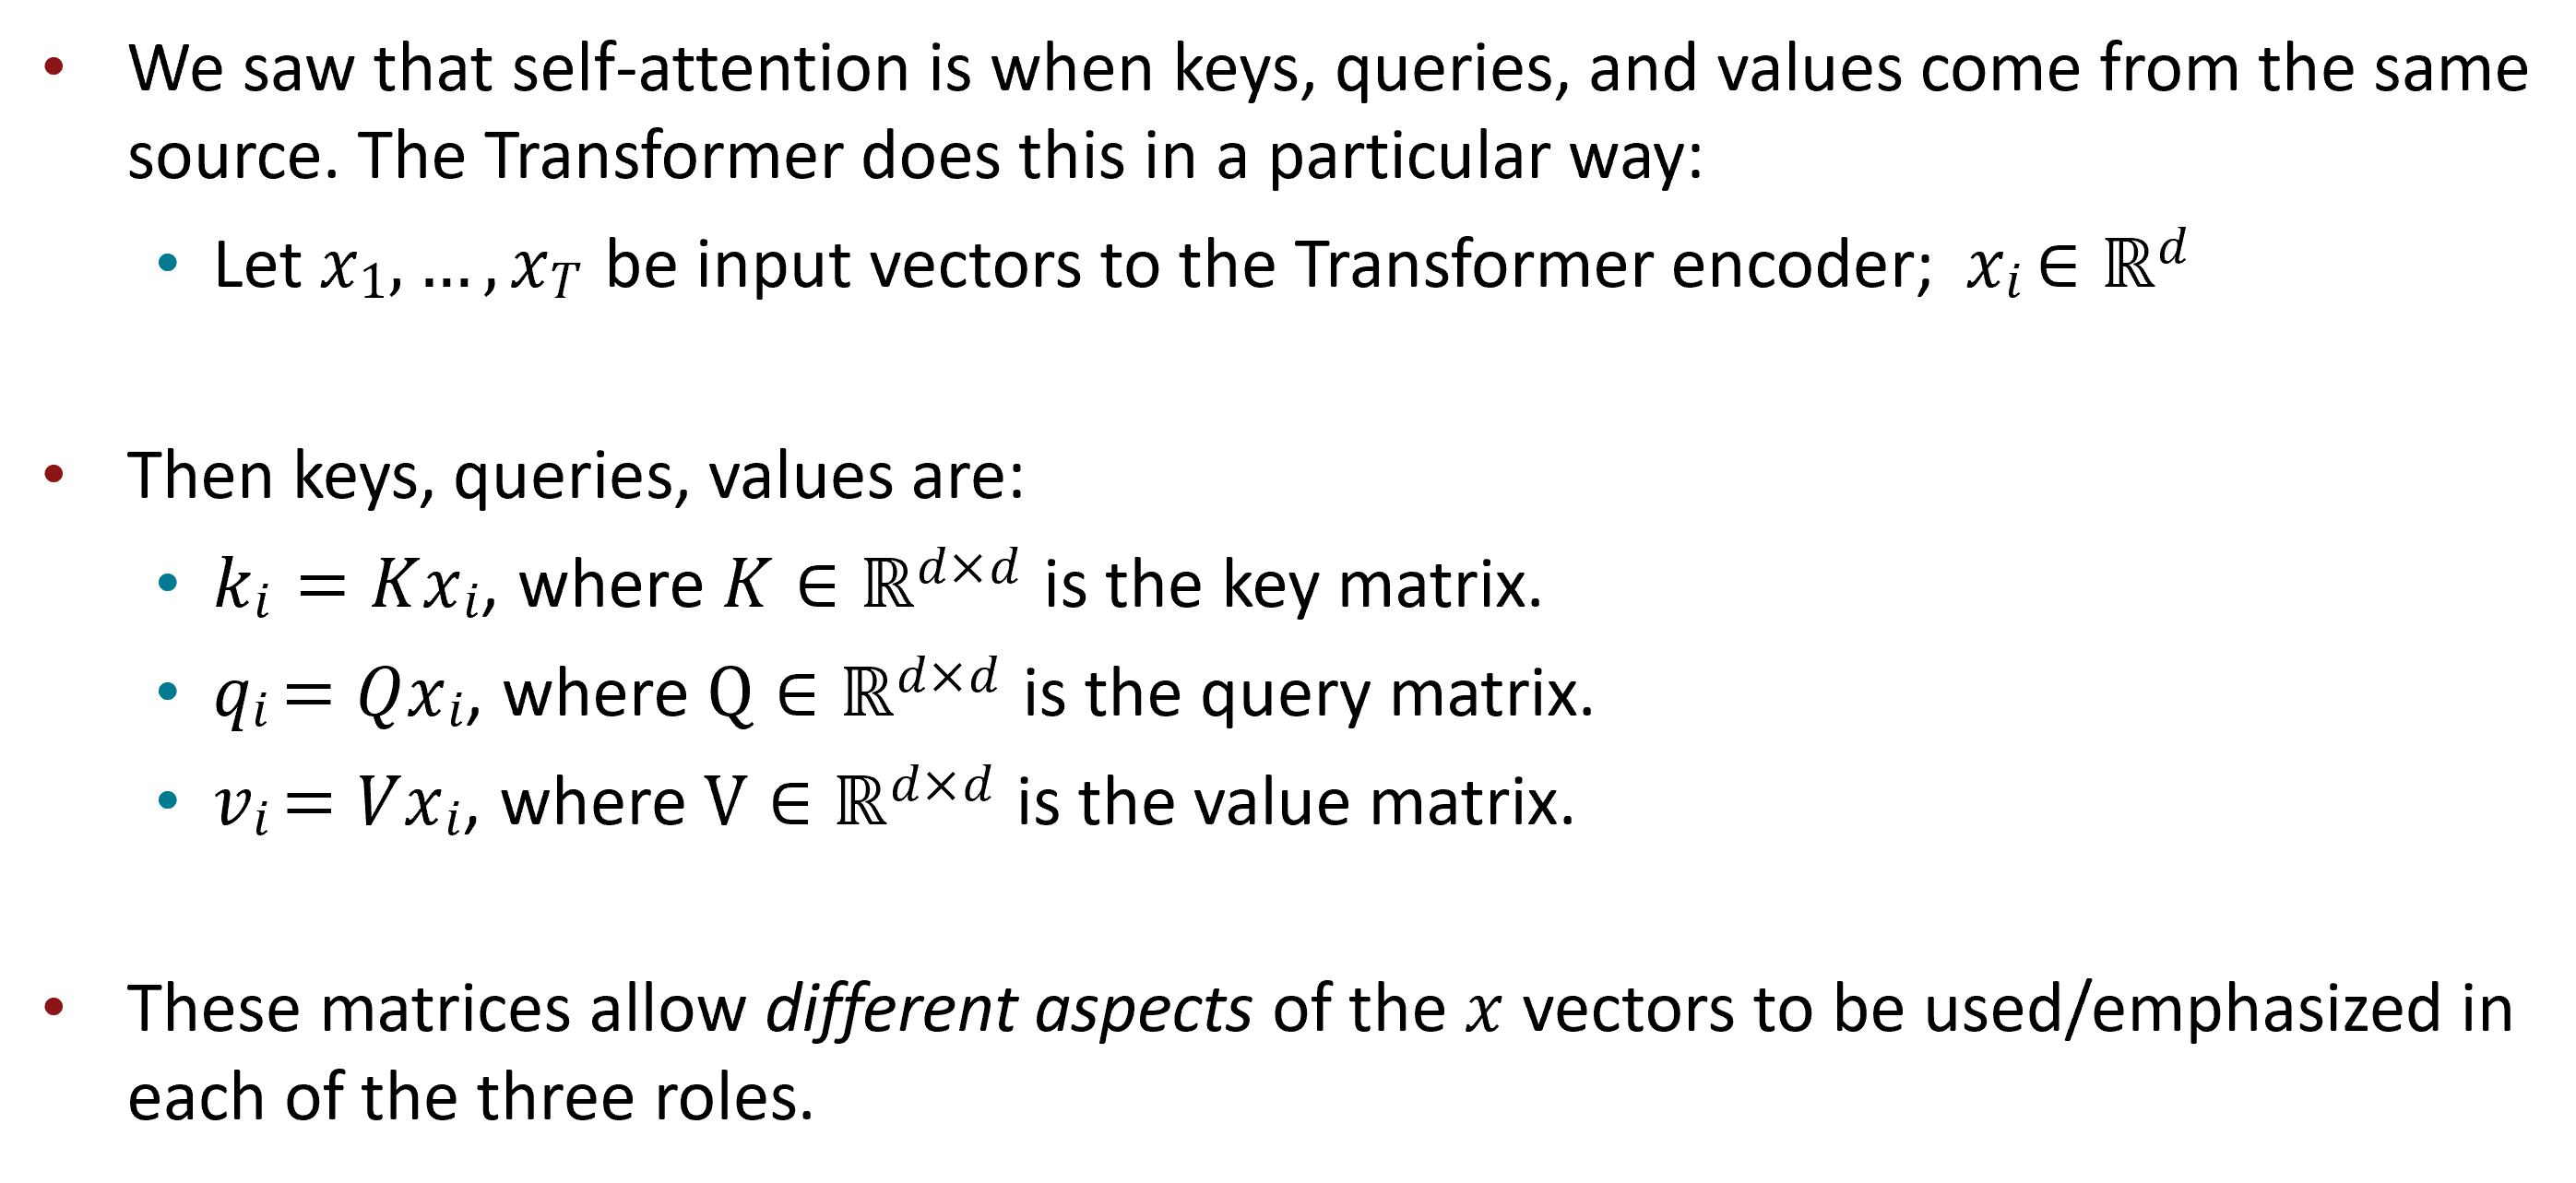
\includegraphics[width=\linewidth,keepaspectratio]{bert75}
			% \end{center}		
			
% % {\tiny (Ref: Language \& Machine Learning - John Hewitt)}

% \end{frame}

% %%%%%%%%%%%%%%%%%%%%%%%%%%%%%%%%%%%%%%%%%%%%%%%%%%%%%%%%%%%
% \begin{frame}[fragile]\frametitle{Key-Query-Value Attention}

			
			% \begin{center}
			% 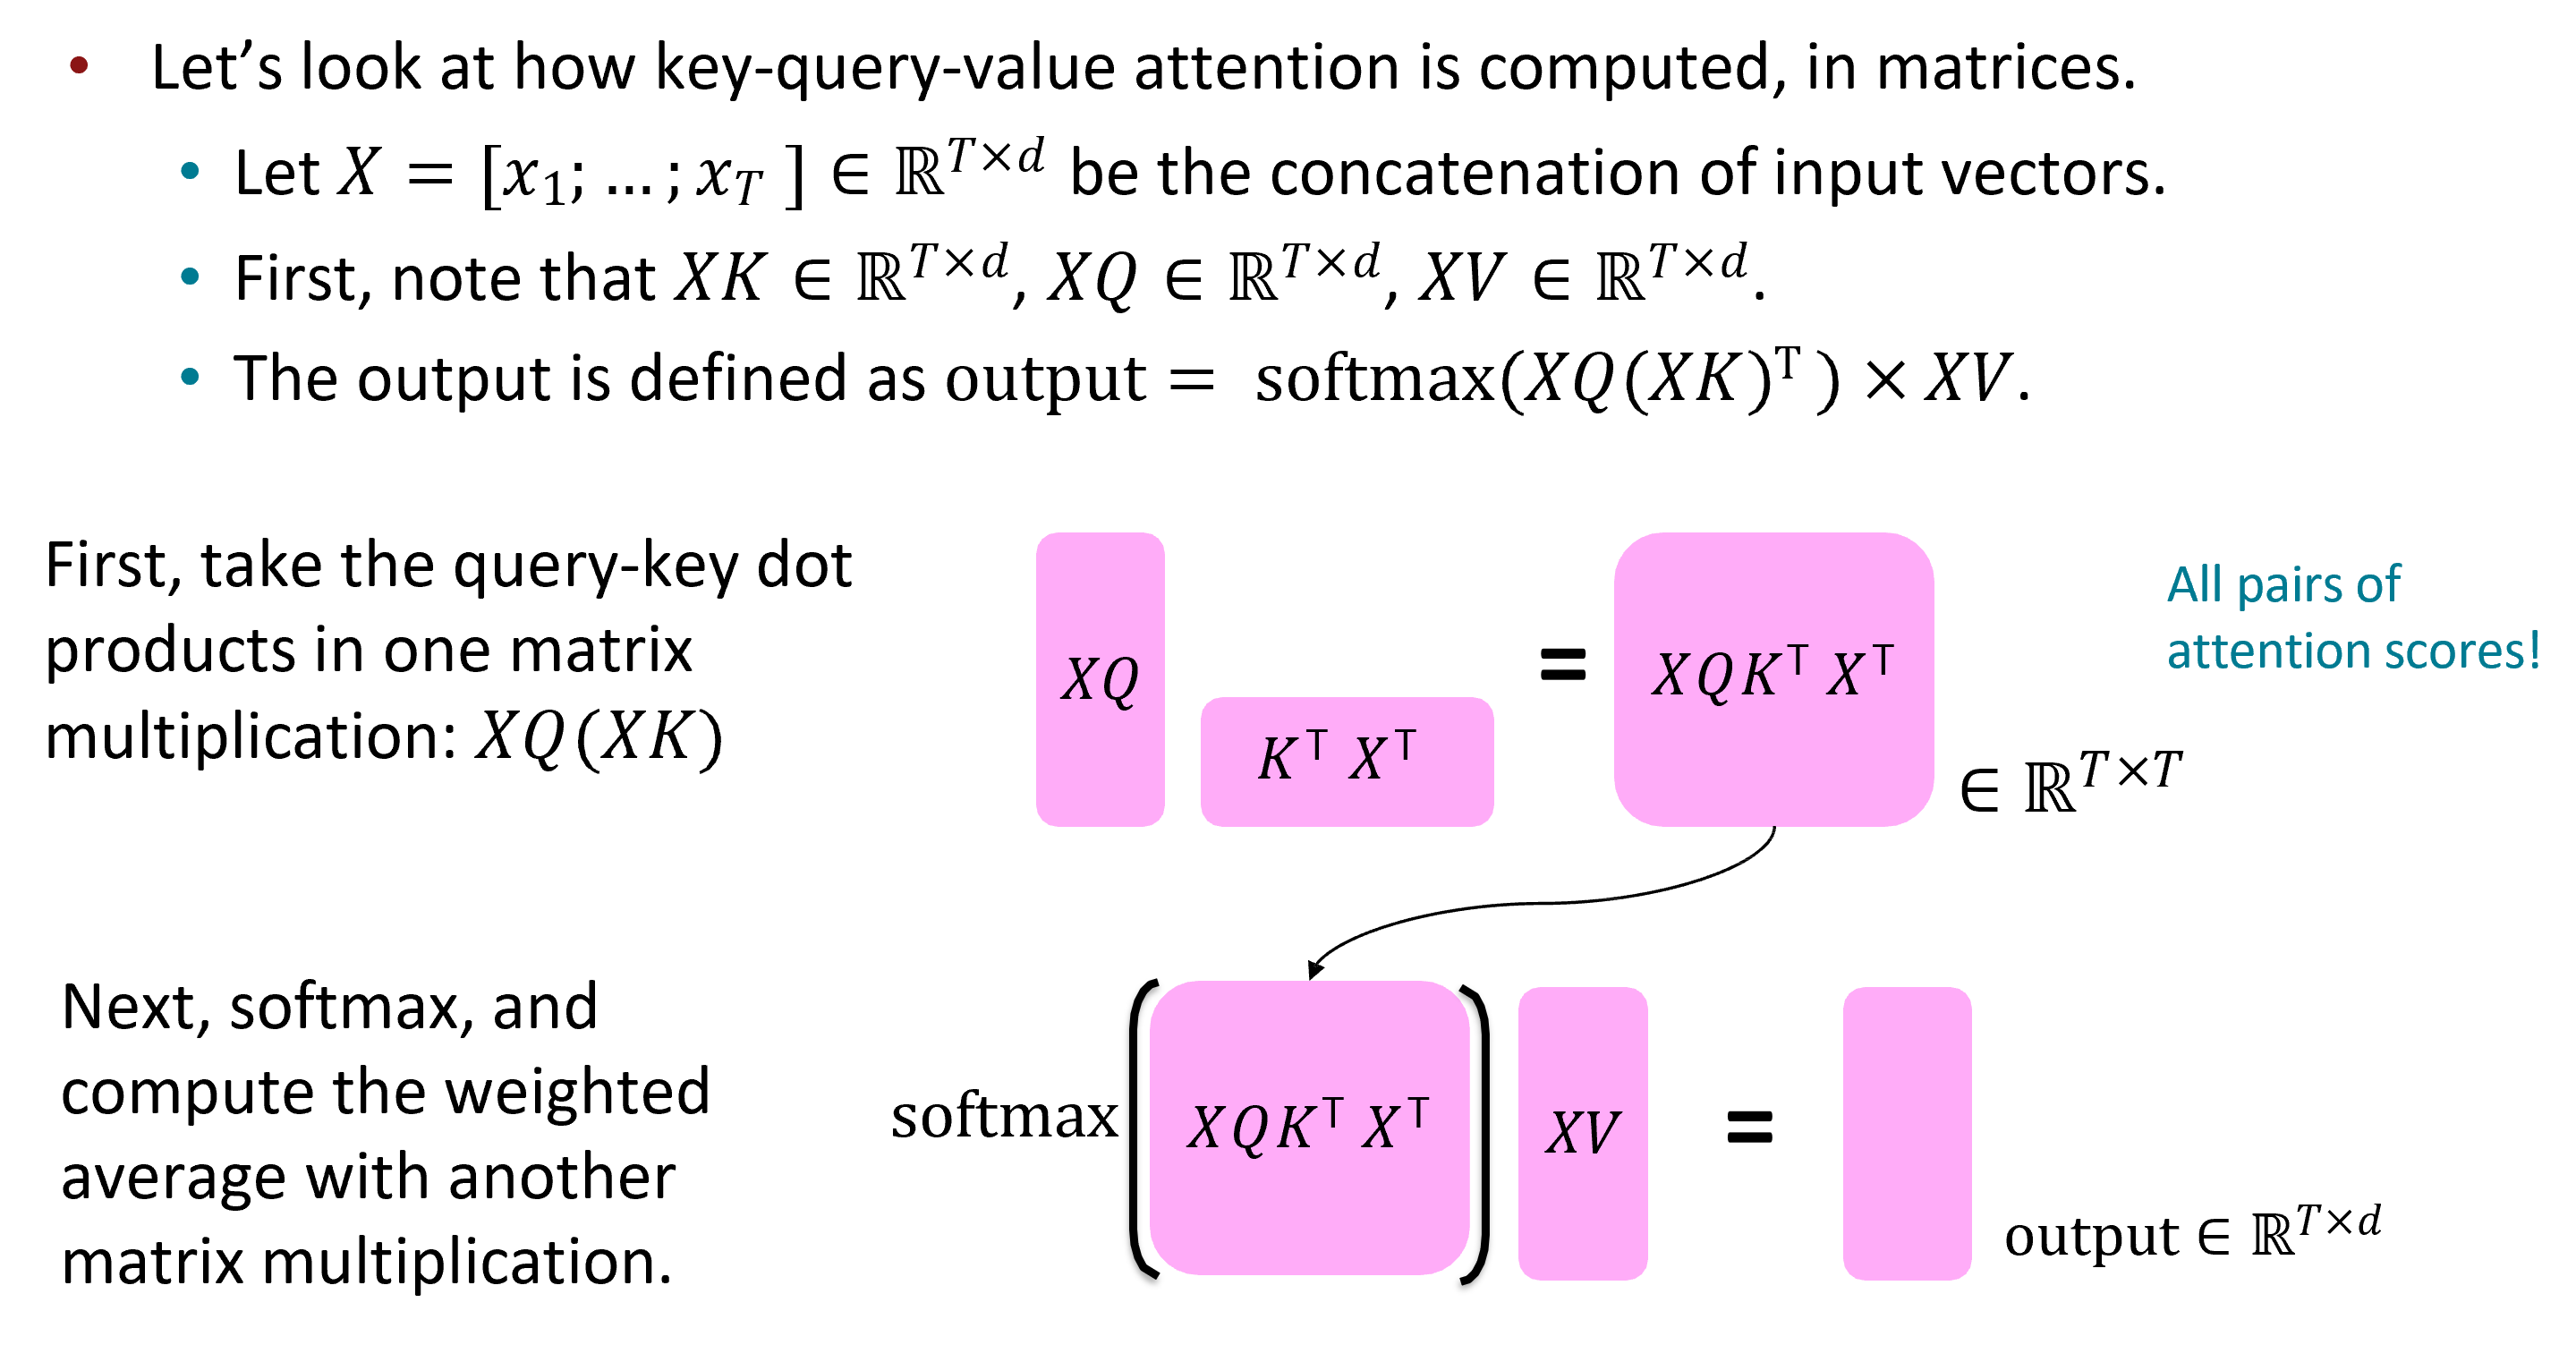
\includegraphics[width=\linewidth,keepaspectratio]{bert76}
			% \end{center}		
			
% % {\tiny (Ref: Language \& Machine Learning - John Hewitt)}

% \end{frame}


%%%%%%%%%%%%%%%%%%%%%%%%%%%%%%%%%%%%%%%%%%%%%%%%%%%%%%%%%%%%%%%%%%%%%%%%%%%%%%%%%%
\begin{frame}[fragile]\frametitle{}
\begin{center}
{\Large Multi-head Attention}
\end{center}
\end{frame}

%%%%%%%%%%%%%%%%%%%%%%%%%%%%%%%%%%%%%%%%%%%%%%%%%%%%%%%%%%%
\begin{frame}[fragile]\frametitle{The Beast With Many Heads}

Having multiple self attention helps:

\begin{columns}
    \begin{column}[T]{0.5\linewidth}
\begin{center}
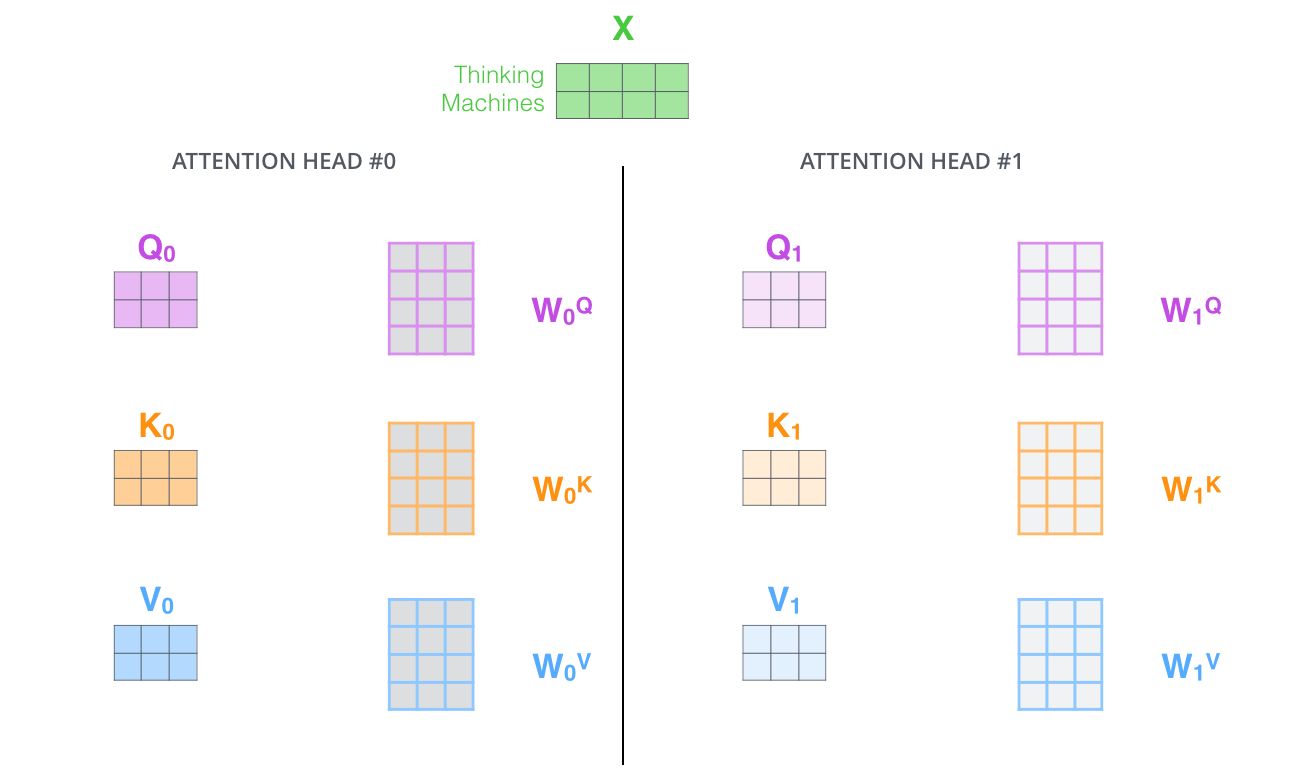
\includegraphics[width=\linewidth,keepaspectratio]{transformer_attention_heads_qkv_jay}


{\tiny (Ref: ``The Illustrated Transformer'' - Jay Alammar)}
\end{center}		

		\end{column}
    \begin{column}[T]{0.5\linewidth}

\begin{itemize}
\item Expands the model’s ability to focus on different positions. Because each weight matrices of Q K V are initialized randomly, they can get settled differently, and also differently for different sentences.
\item Paper uses 8 heads in a single multi-head self attention cell.
\item ie Each of these sets is randomly initialized. Then, after training, each set is used to project the input embeddings (or vectors from lower encoders/decoders) into a different representation subspace.
\end{itemize}
    \end{column}
  \end{columns}
\end{frame}

%%%%%%%%%%%%%%%%%%%%%%%%%%%%%%%%%%%%%%%%%%%%%%%%%%%%%%%%%%%
\begin{frame}[fragile]\frametitle{The Beast With Many Heads}

Having multiple self attention helps:

\begin{columns}
    \begin{column}[T]{0.5\linewidth}
\begin{center}
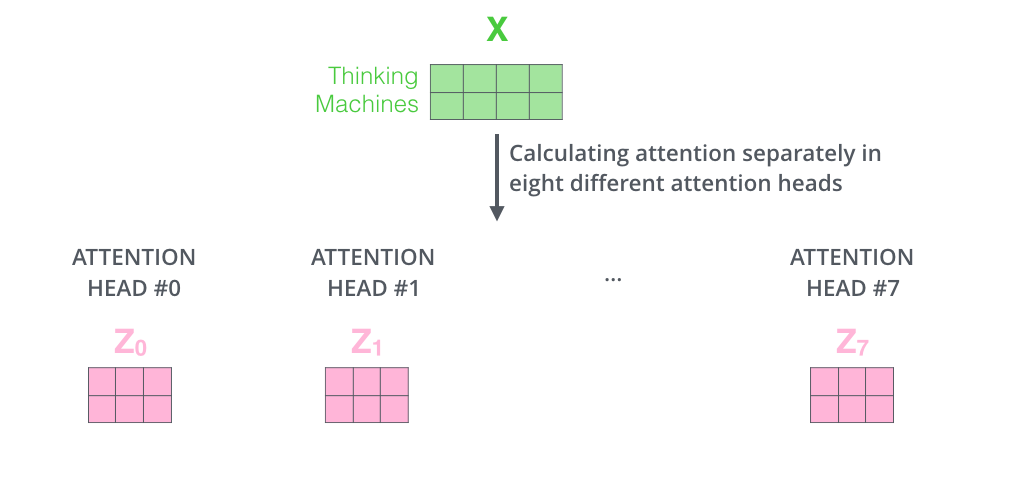
\includegraphics[width=\linewidth,keepaspectratio]{transformer_attention_heads_z_jay}


{\tiny (Ref: ``The Illustrated Transformer'' - Jay Alammar)}
\end{center}		

		\end{column}
    \begin{column}[T]{0.5\linewidth}

\begin{itemize}
\item One problem though. 
\item The next feed-forward layer is not expecting eight matrices – it’s expecting a single matrix (a vector for each word). So we need a way to condense these eight down into a single matrix.
\item How do we do that? 
\end{itemize}
    \end{column}
  \end{columns}
\end{frame}

%%%%%%%%%%%%%%%%%%%%%%%%%%%%%%%%%%%%%%%%%%%%%%%%%%%%%%%%%%%
\begin{frame}[fragile]\frametitle{The Beast With Many Heads}

Having multiple self attention helps:

\begin{columns}
    \begin{column}[T]{0.5\linewidth}
\begin{center}
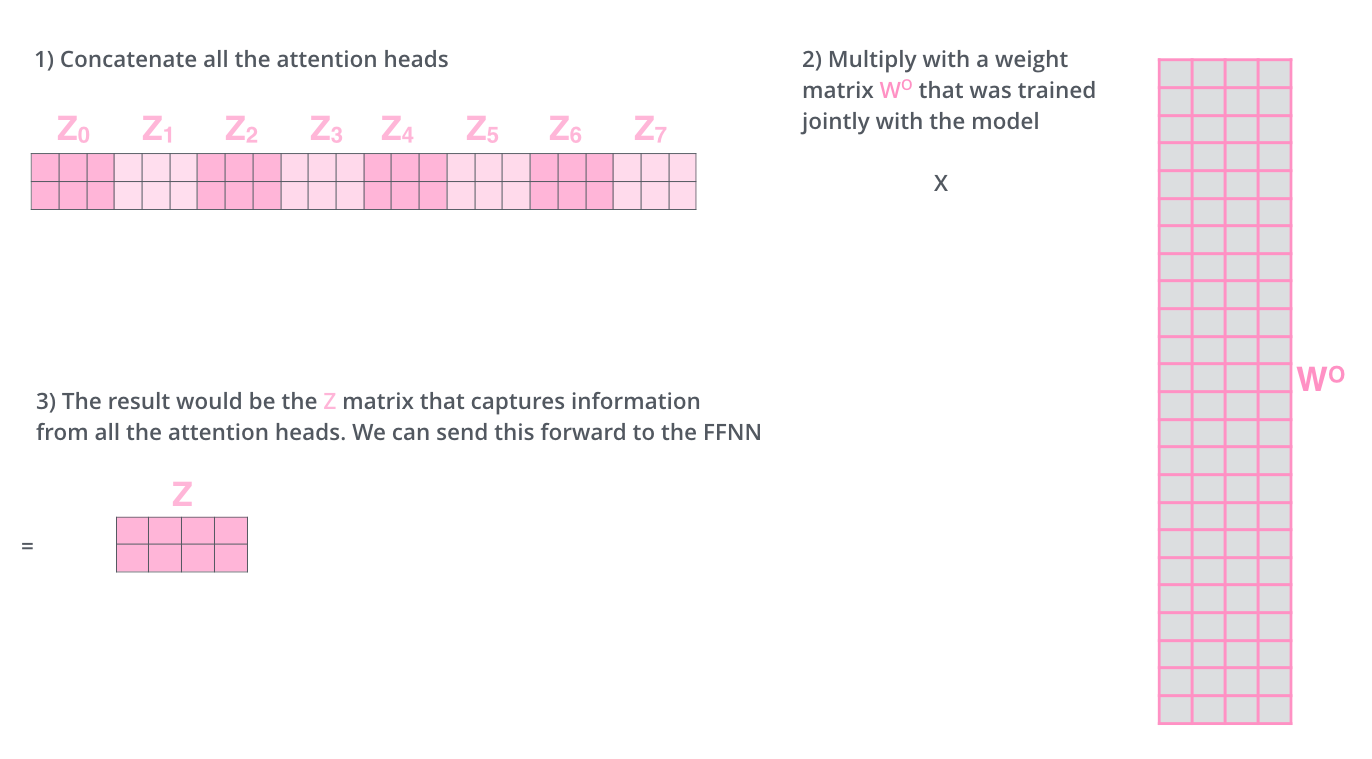
\includegraphics[width=\linewidth,keepaspectratio]{transformer_attention_heads_weight_matrix_o_jay}


{\tiny (Ref: ``The Illustrated Transformer'' - Jay Alammar)}
\end{center}		

		\end{column}
    \begin{column}[T]{0.5\linewidth}

\begin{itemize}
\item  We concat the matrices then multiply them by an additional weights matrix $W^O$.
\end{itemize}
    \end{column}
  \end{columns}
\end{frame}


%%%%%%%%%%%%%%%%%%%%%%%%%%%%%%%%%%%%%%%%%%%%%%%%%%%%%%%%%%%
\begin{frame}[fragile]\frametitle{Self Attention in Summary}


\begin{center}
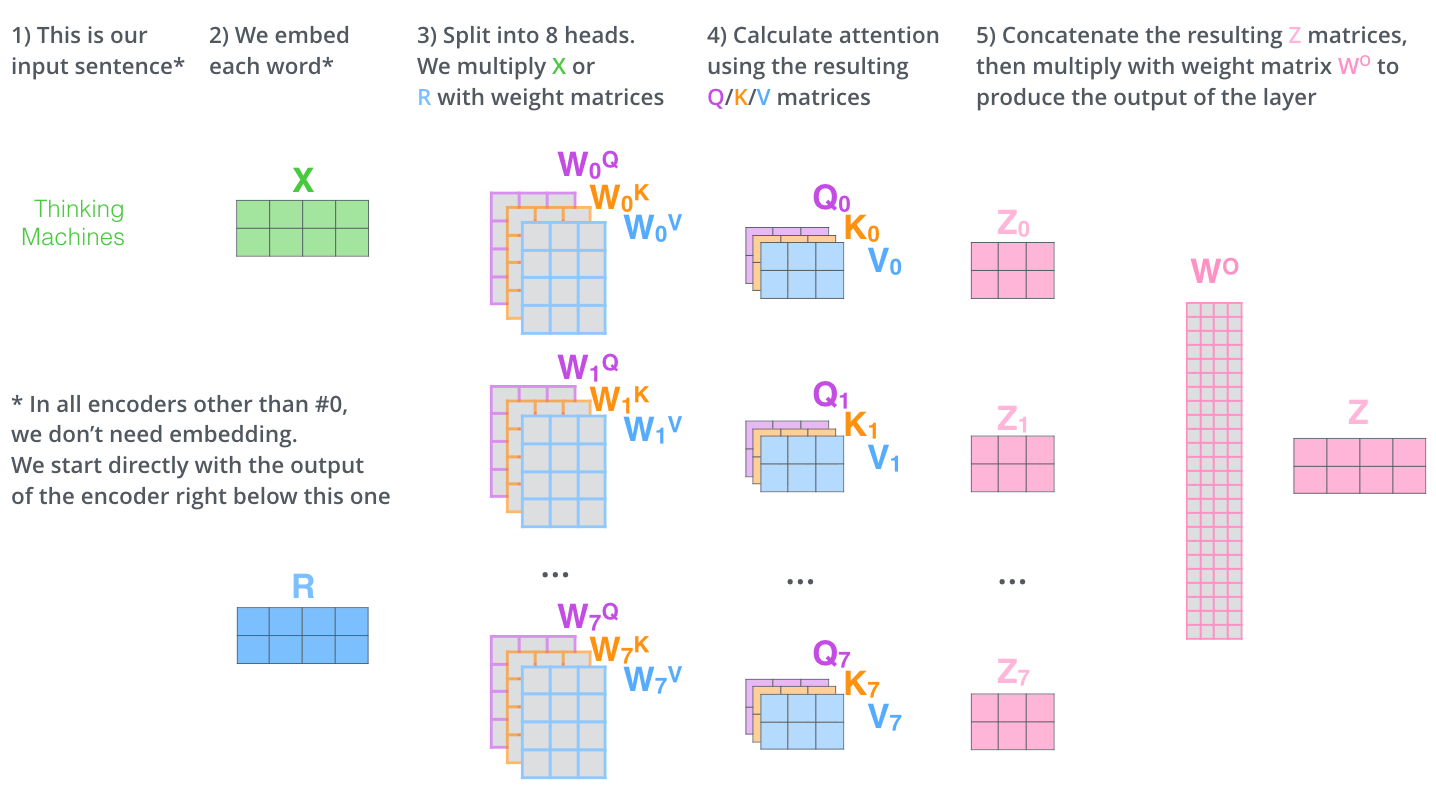
\includegraphics[width=\linewidth,keepaspectratio]{transformer_multi-headed_self-attention-recap_jay}


{\tiny (Ref: ``The Illustrated Transformer'' - Jay Alammar)}
\end{center}	


* Please note that in the diagram the Embedding vectors $X$ also include positional encoding incorporated inside.	

\end{frame}


%%%%%%%%%%%%%%%%%%%%%%%%%%%%%%%%%%%%%%%%%%%%%%%%%%%%%%%%%%%
\begin{frame}[fragile]\frametitle{Self Attention in Summary Example}


\begin{center}
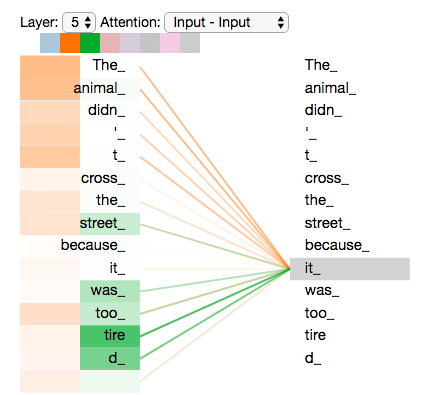
\includegraphics[width=\linewidth,keepaspectratio]{transformer_self-attention_visualization_2_jay}


{\tiny (Ref: ``The Illustrated Transformer'' - Jay Alammar)}
\end{center}	


As we encode the word "it", one attention head is focusing most on "the animal", while another is focusing on "tired" -- in a sense, the model's representation of the word "it" bakes in some of the representation of both "animal" and "tired".

\end{frame}

%%%%%%%%%%%%%%%%%%%%%%%%%%%%%%%%%%%%%%%%%%%%%%%%%%%%%%%%%%%
\begin{frame}[fragile]\frametitle{Self Attention in Summary Example}



\begin{center}
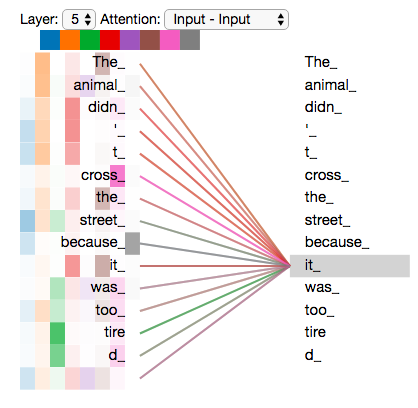
\includegraphics[width=\linewidth,keepaspectratio]{transformer_self-attention_visualization_3_jay}


{\tiny (Ref: ``The Illustrated Transformer'' - Jay Alammar)}
\end{center}	

If we add all the attention heads to the picture, however, things can be harder to interpret, but thats what happens.

This is how Self-Attention block generates, ``attended'' vectors.

\end{frame}

% %%%%%%%%%%%%%%%%%%%%%%%%%%%%%%%%%%%%%%%%%%%%%%%%%%%%%%%%%%%
% \begin{frame}[fragile]\frametitle{Multi-headed attention}

			
			% \begin{center}
			% 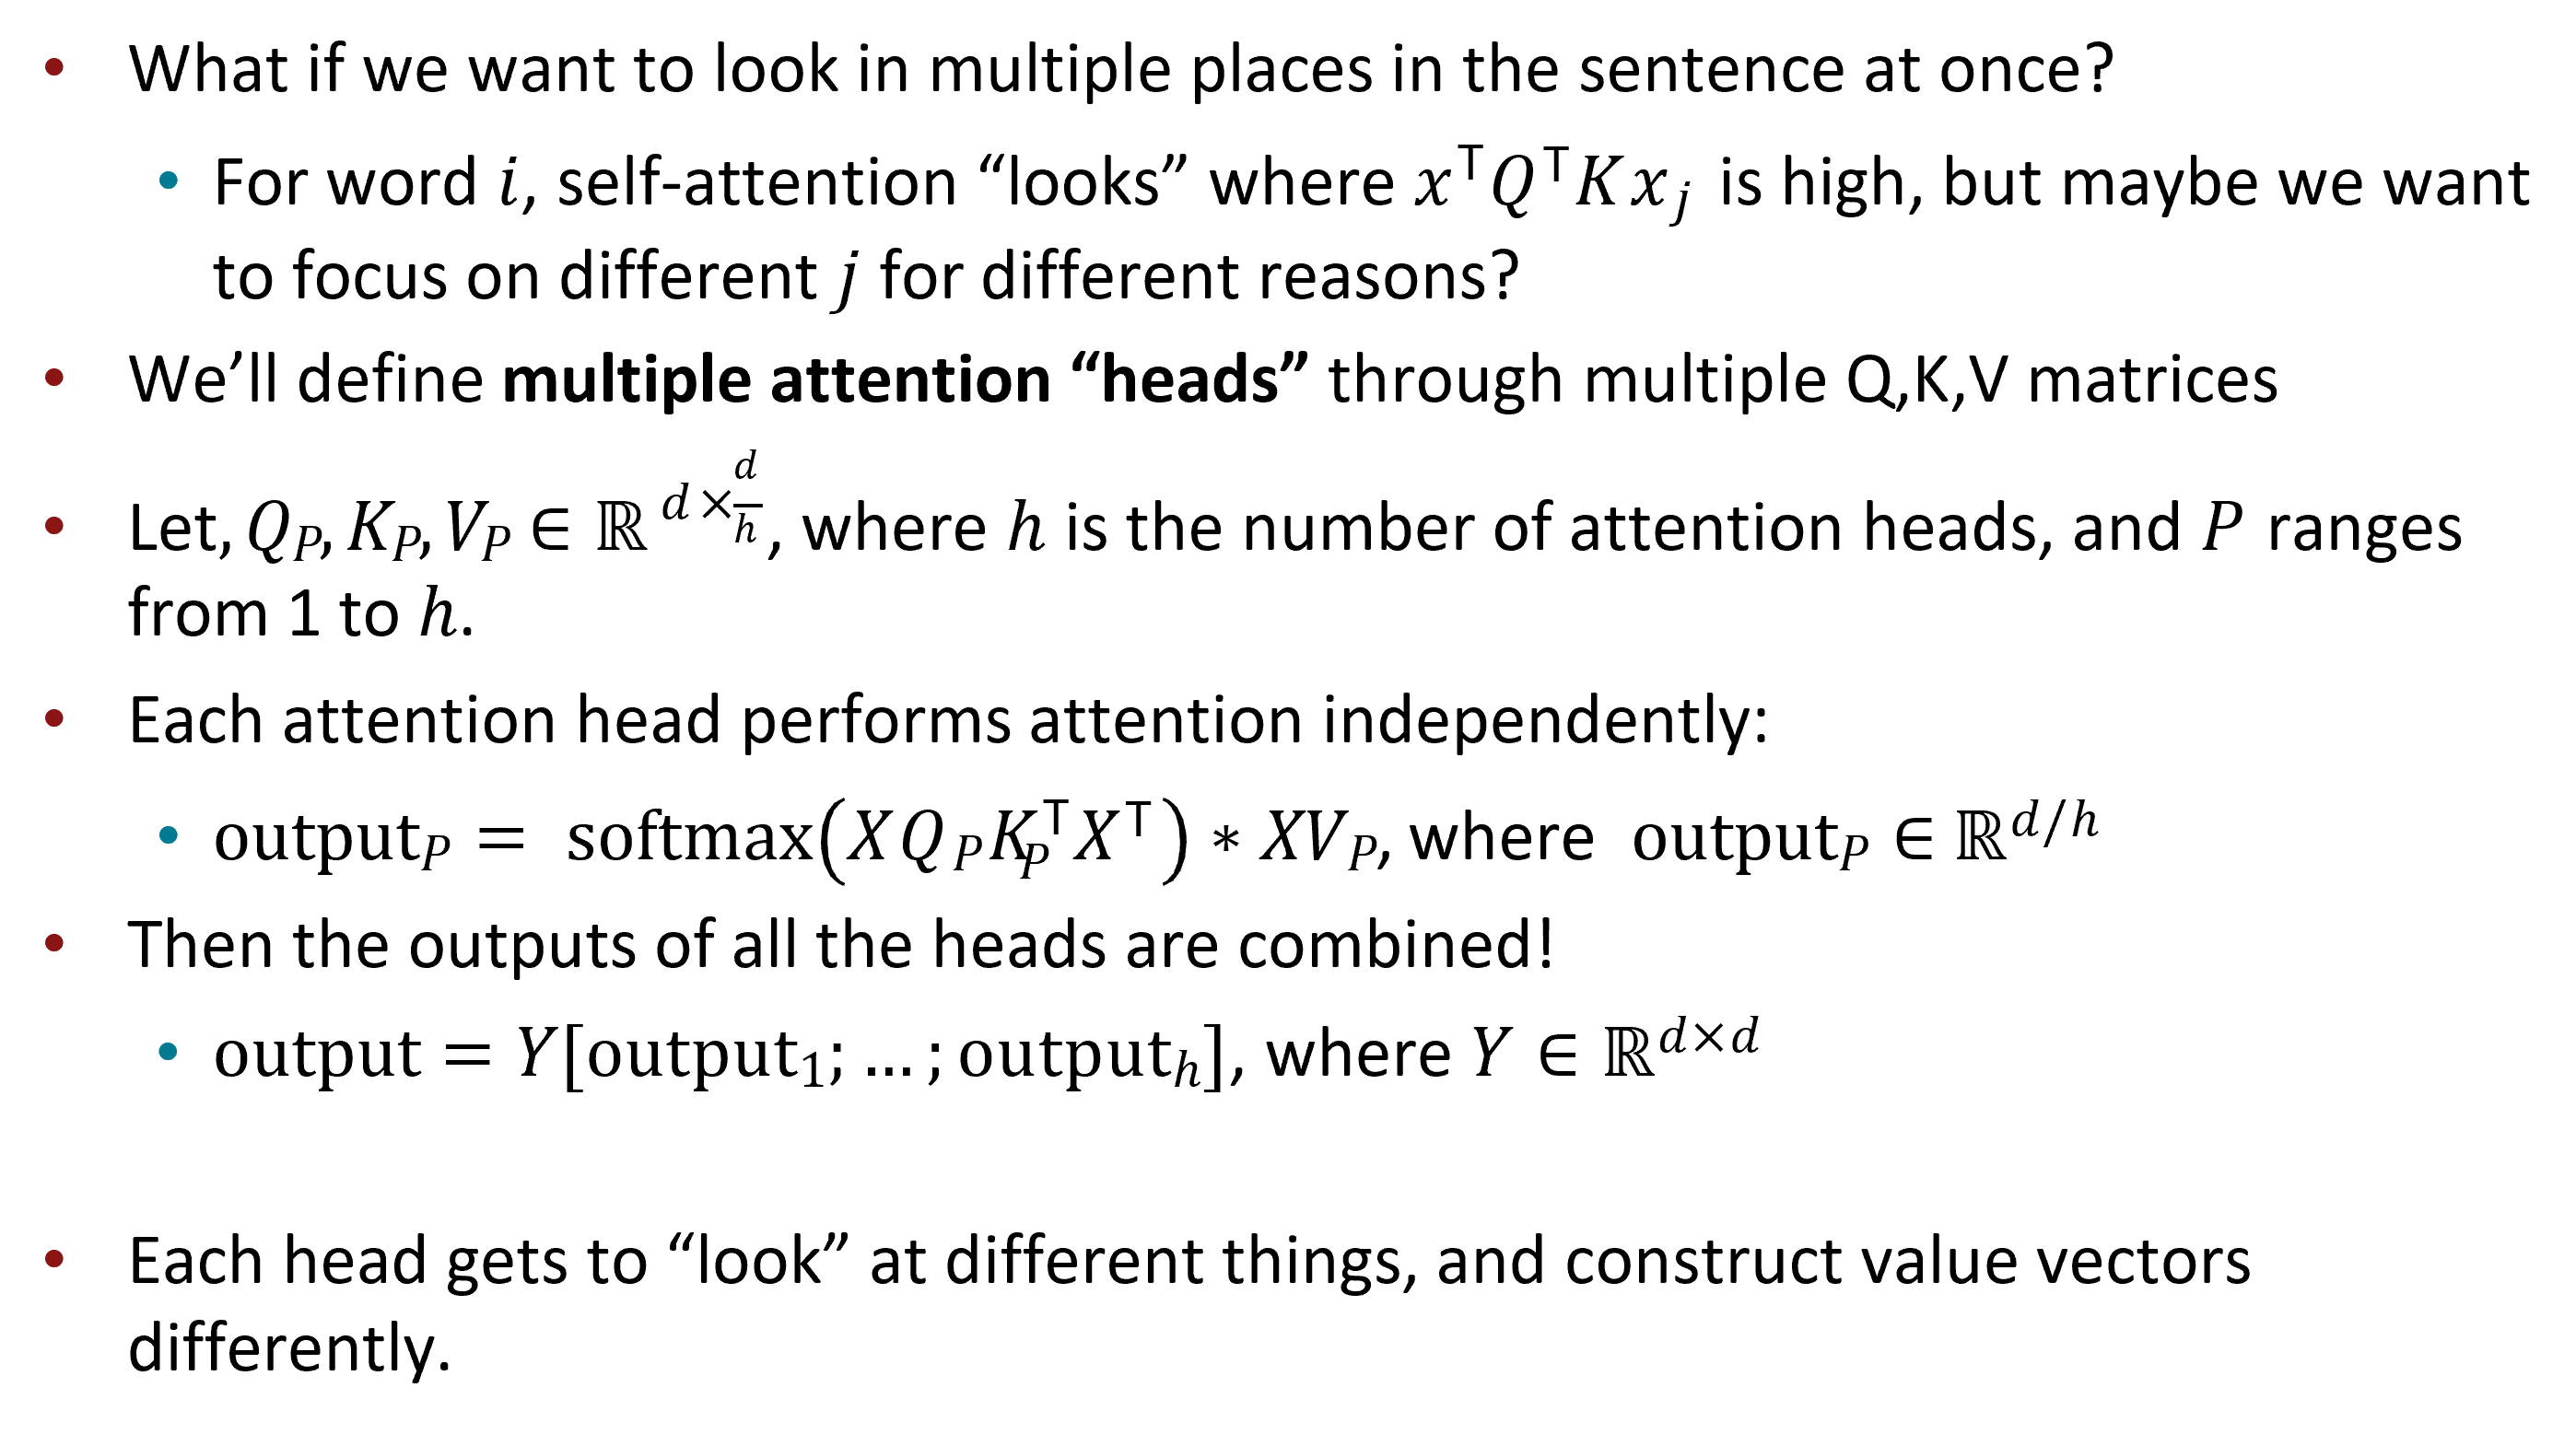
\includegraphics[width=\linewidth,keepaspectratio]{bert77}
			% \end{center}		
			
% % {\tiny (Ref: Language \& Machine Learning - John Hewitt)}

% \end{frame}

% %%%%%%%%%%%%%%%%%%%%%%%%%%%%%%%%%%%%%%%%%%%%%%%%%%%%%%%%%%%
% \begin{frame}[fragile]\frametitle{The Transformer Encoder: Multi-headed attention}

			
			% \begin{center}
			% 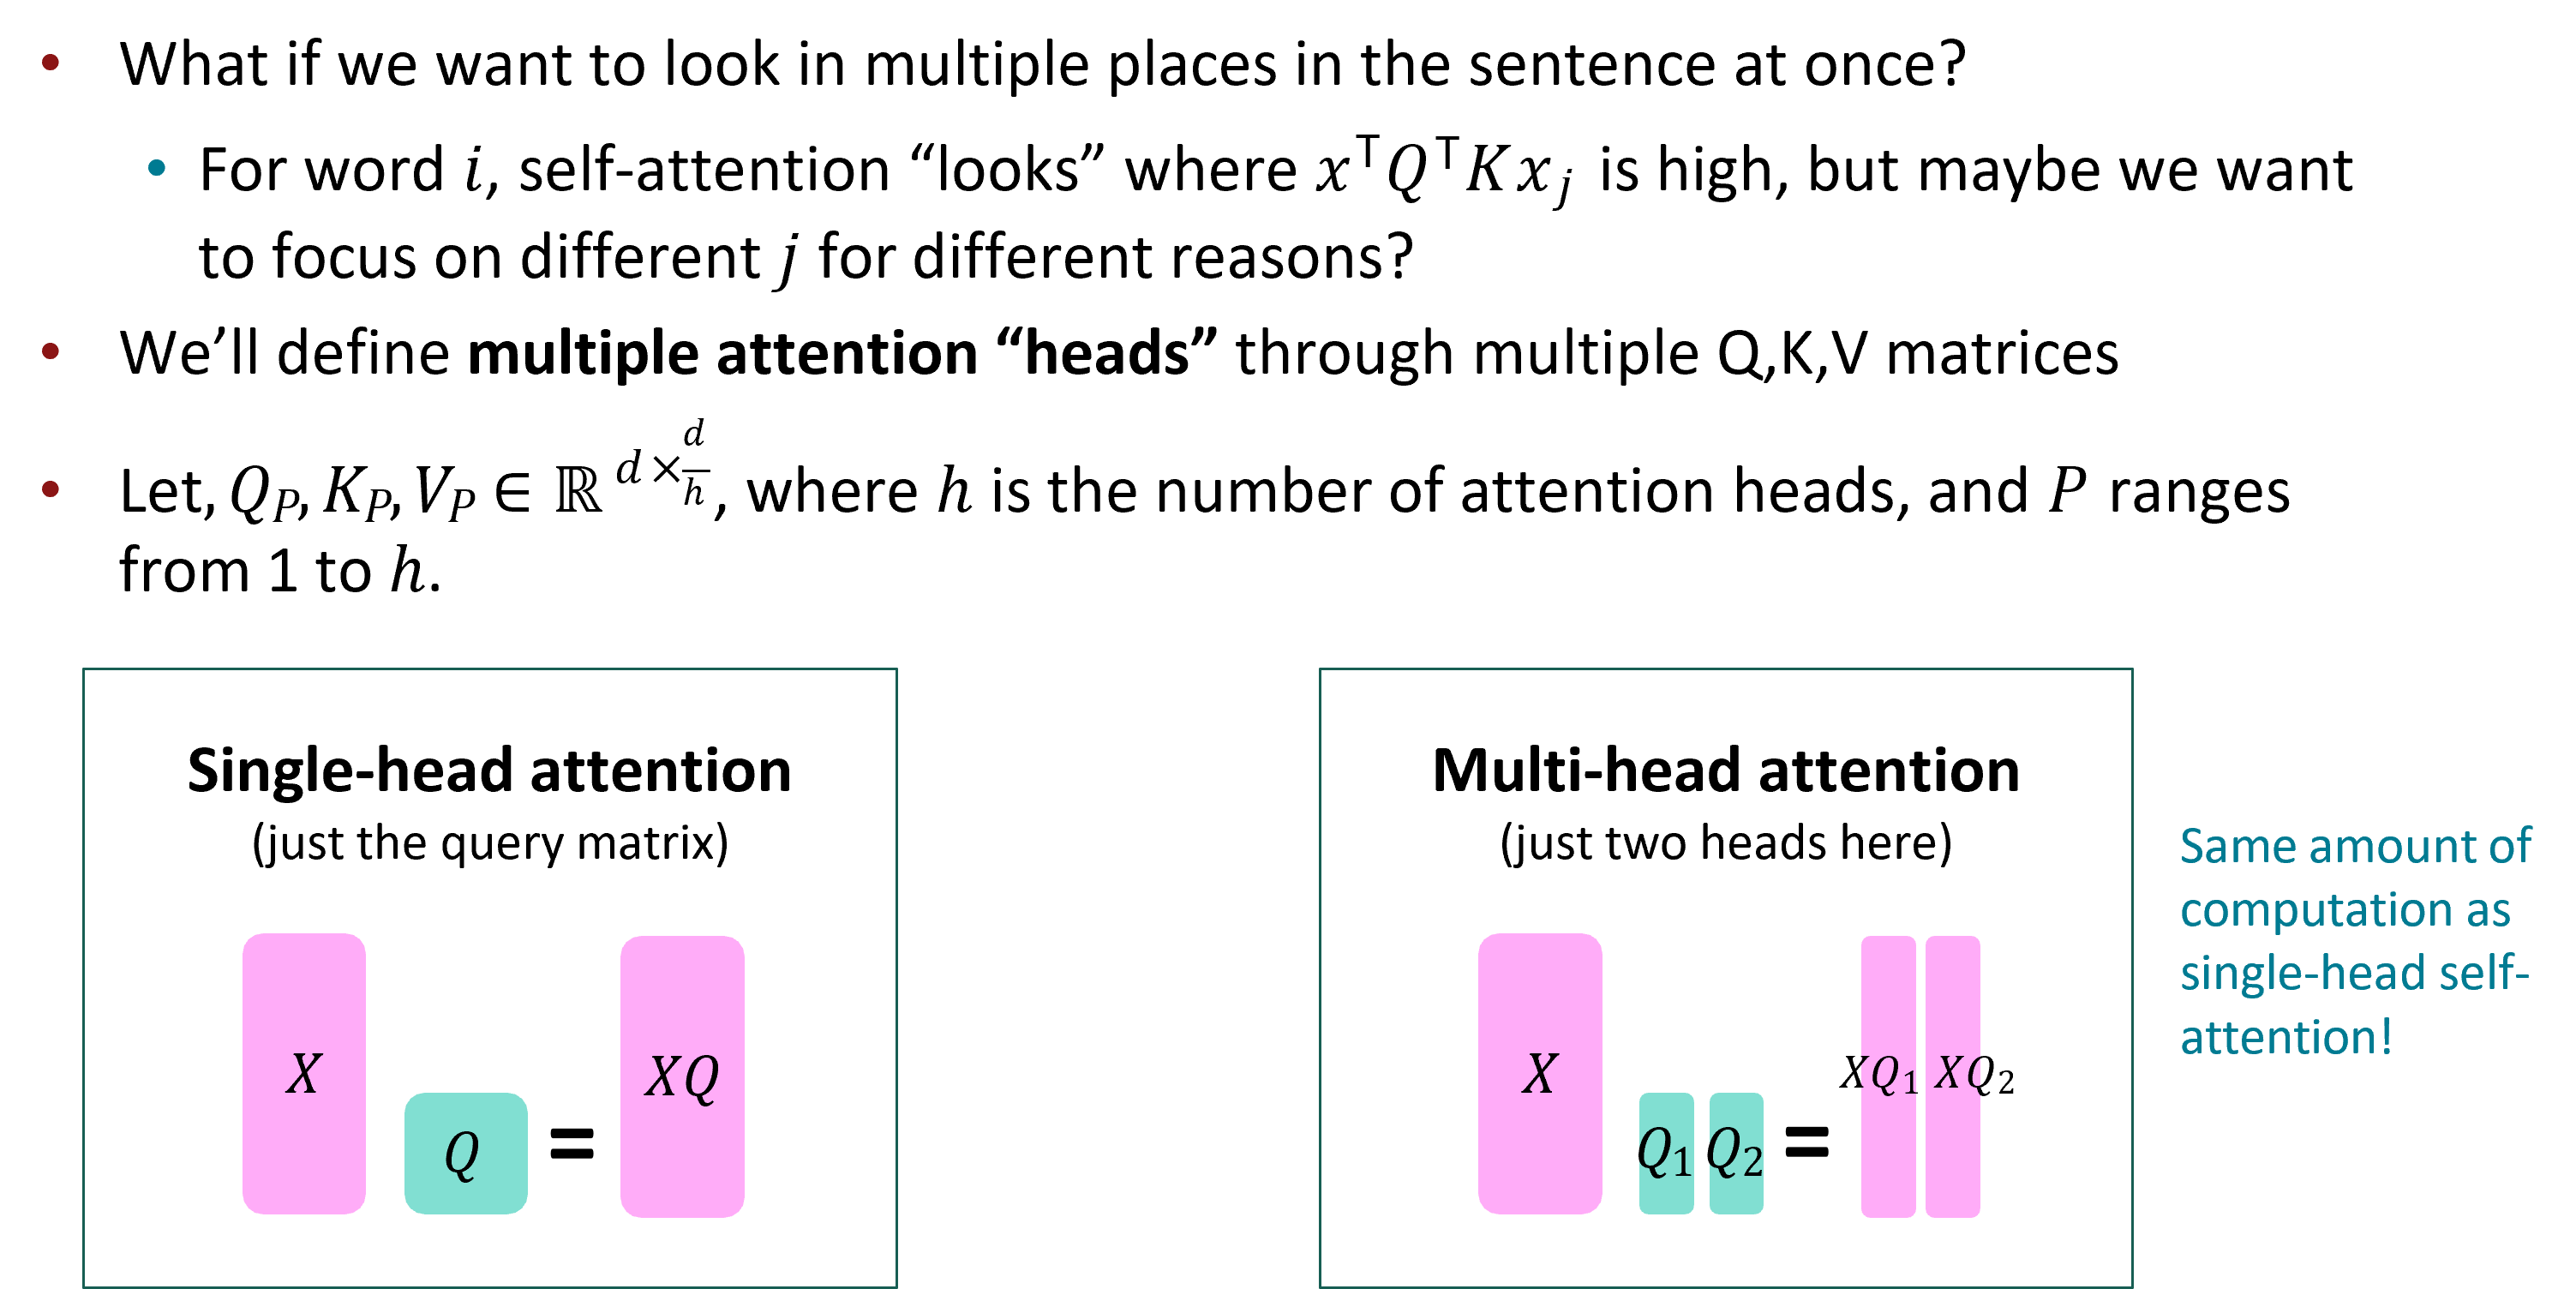
\includegraphics[width=\linewidth,keepaspectratio]{bert78}
			% \end{center}		
			
% % {\tiny (Ref: Language \& Machine Learning - John Hewitt)}

% \end{frame}

% %%%%%%%%%%%%%%%%%%%%%%%%%%%%%%%%%%%%%%%%%%%%%%%%%%%%%%%%%%%
% \begin{frame}[fragile]\frametitle{Attention visualization in layer 5}

			
			% \begin{center}
			% 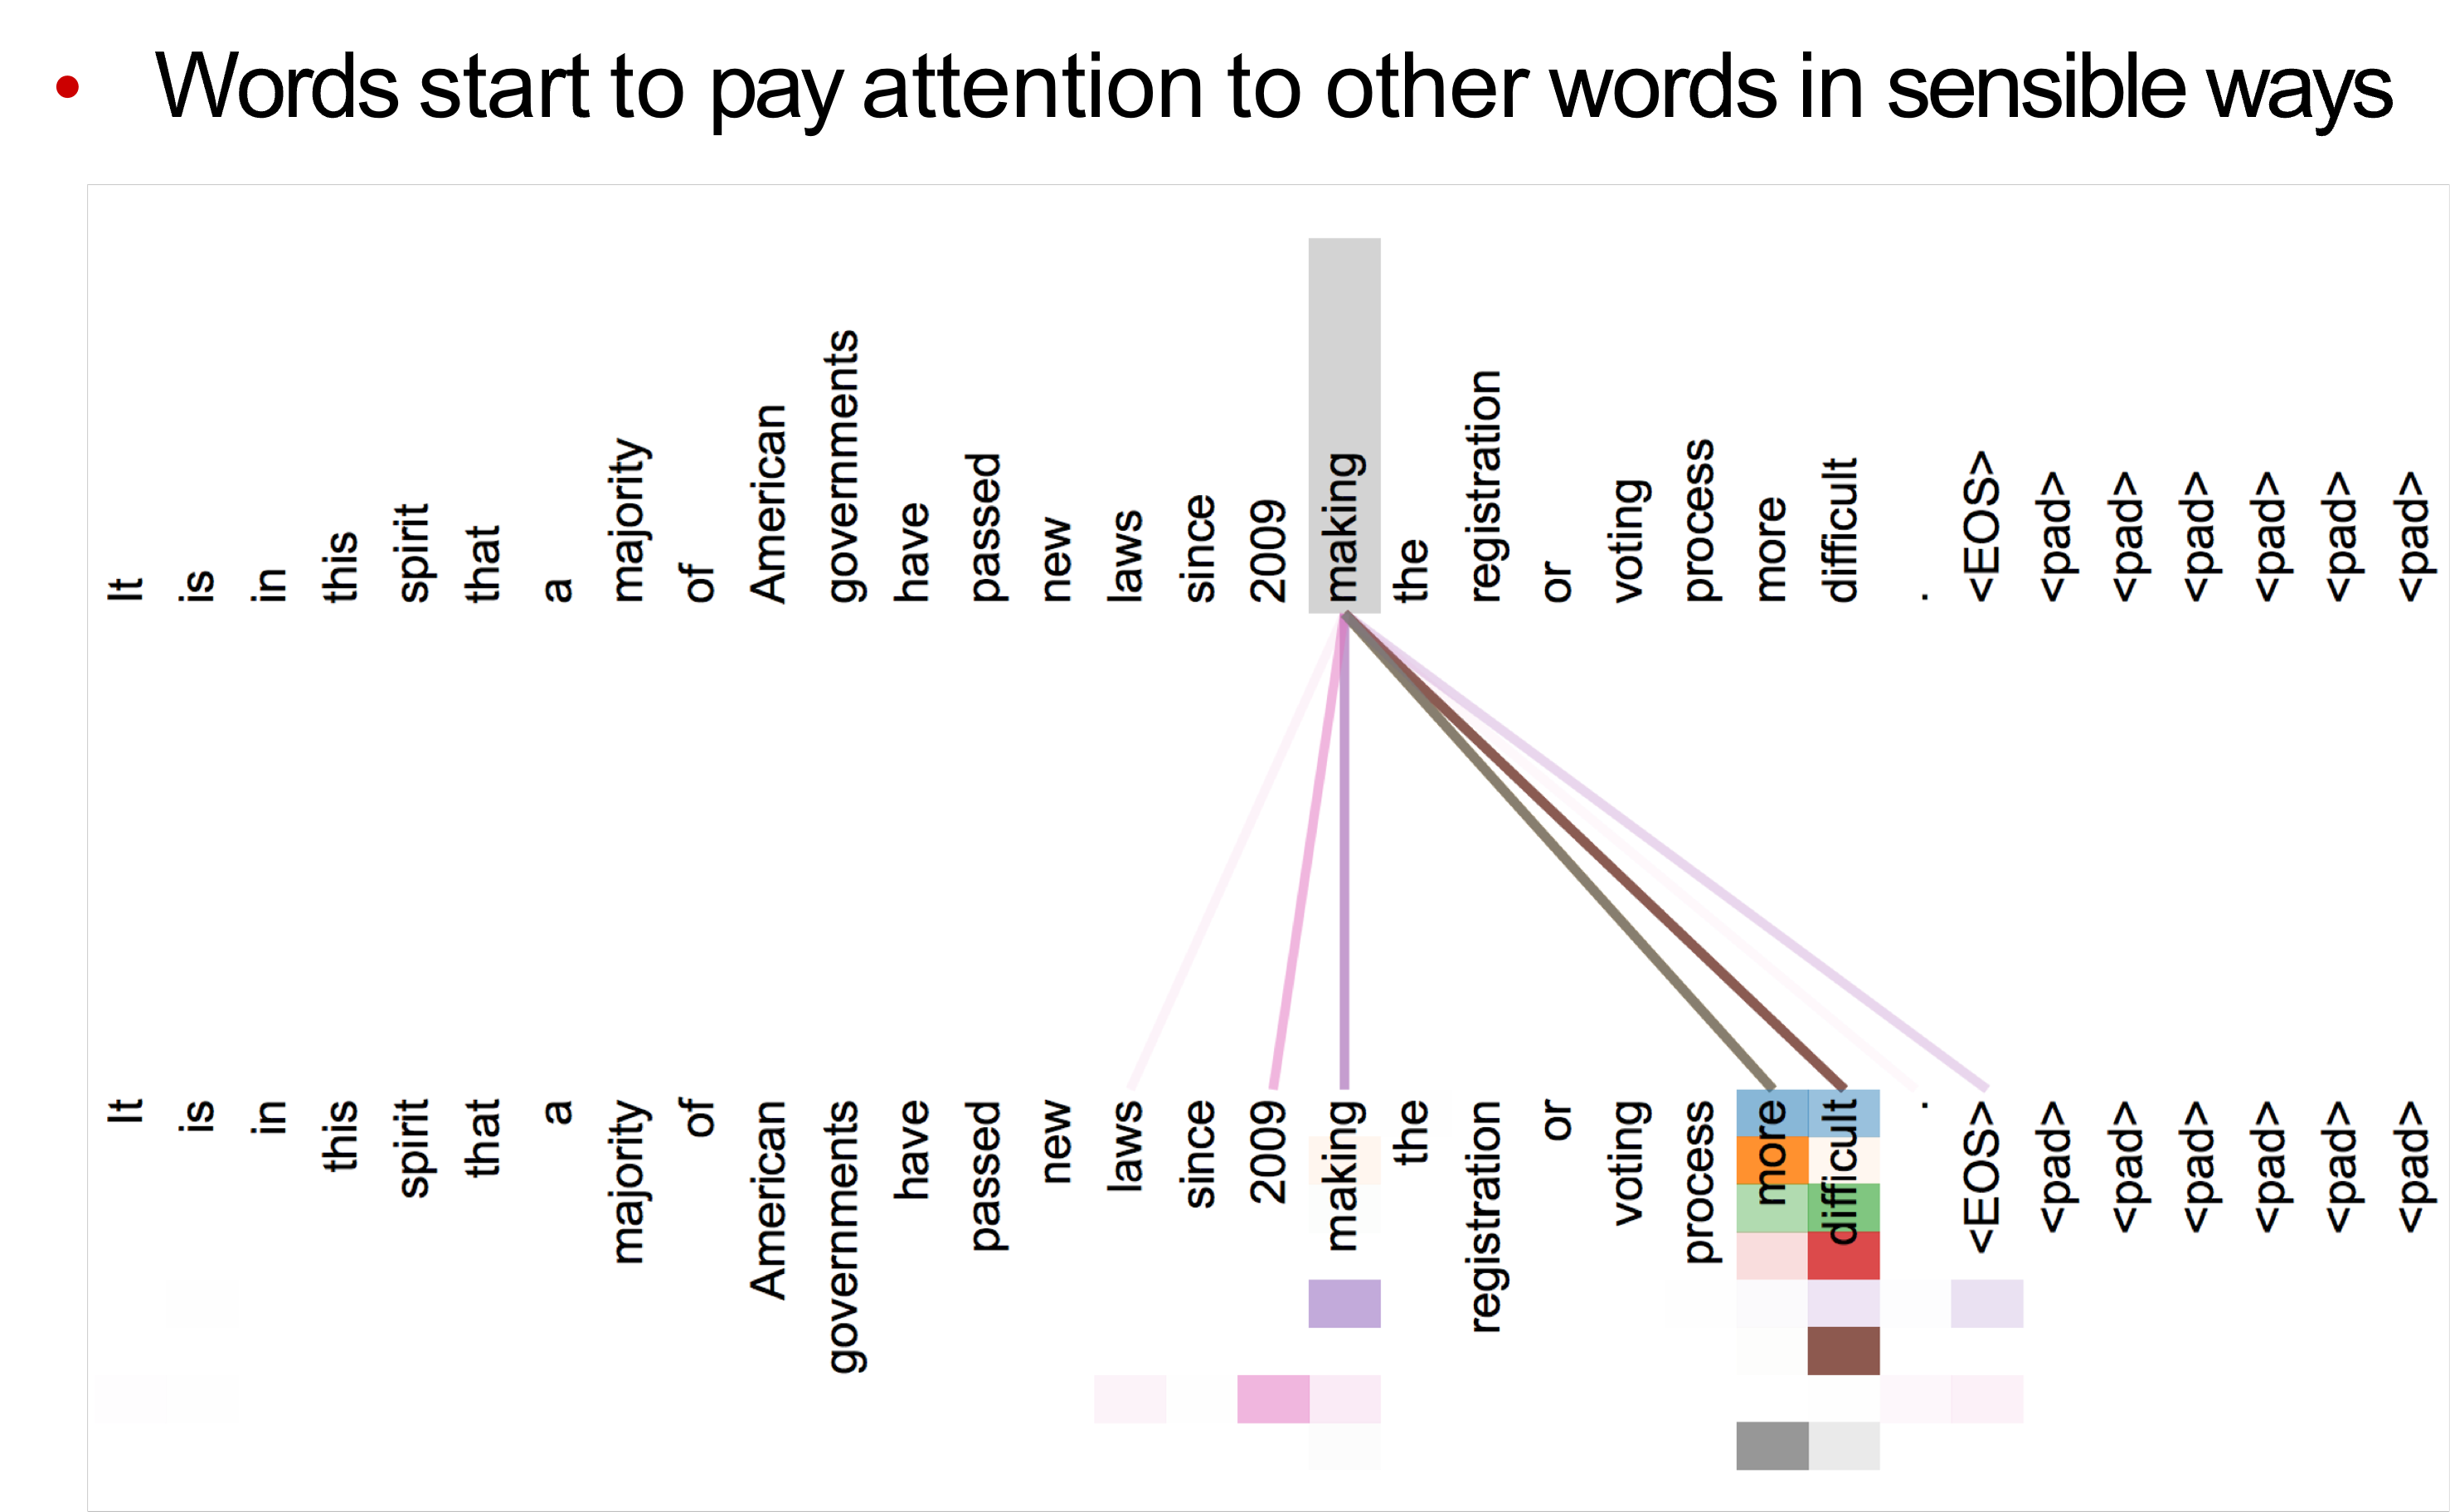
\includegraphics[width=0.8\linewidth,keepaspectratio]{bert79}
			% \end{center}		
			
			% % {\tiny (Ref: CS224n: Natural Language Processing with Deep Learning - Christopher Manning)}

% \end{frame}

% %%%%%%%%%%%%%%%%%%%%%%%%%%%%%%%%%%%%%%%%%%%%%%%%%%%%%%%%%%%
% \begin{frame}[fragile]\frametitle{Attention visualization: Implicit anaphora resolution}

			
			% \begin{center}
			% 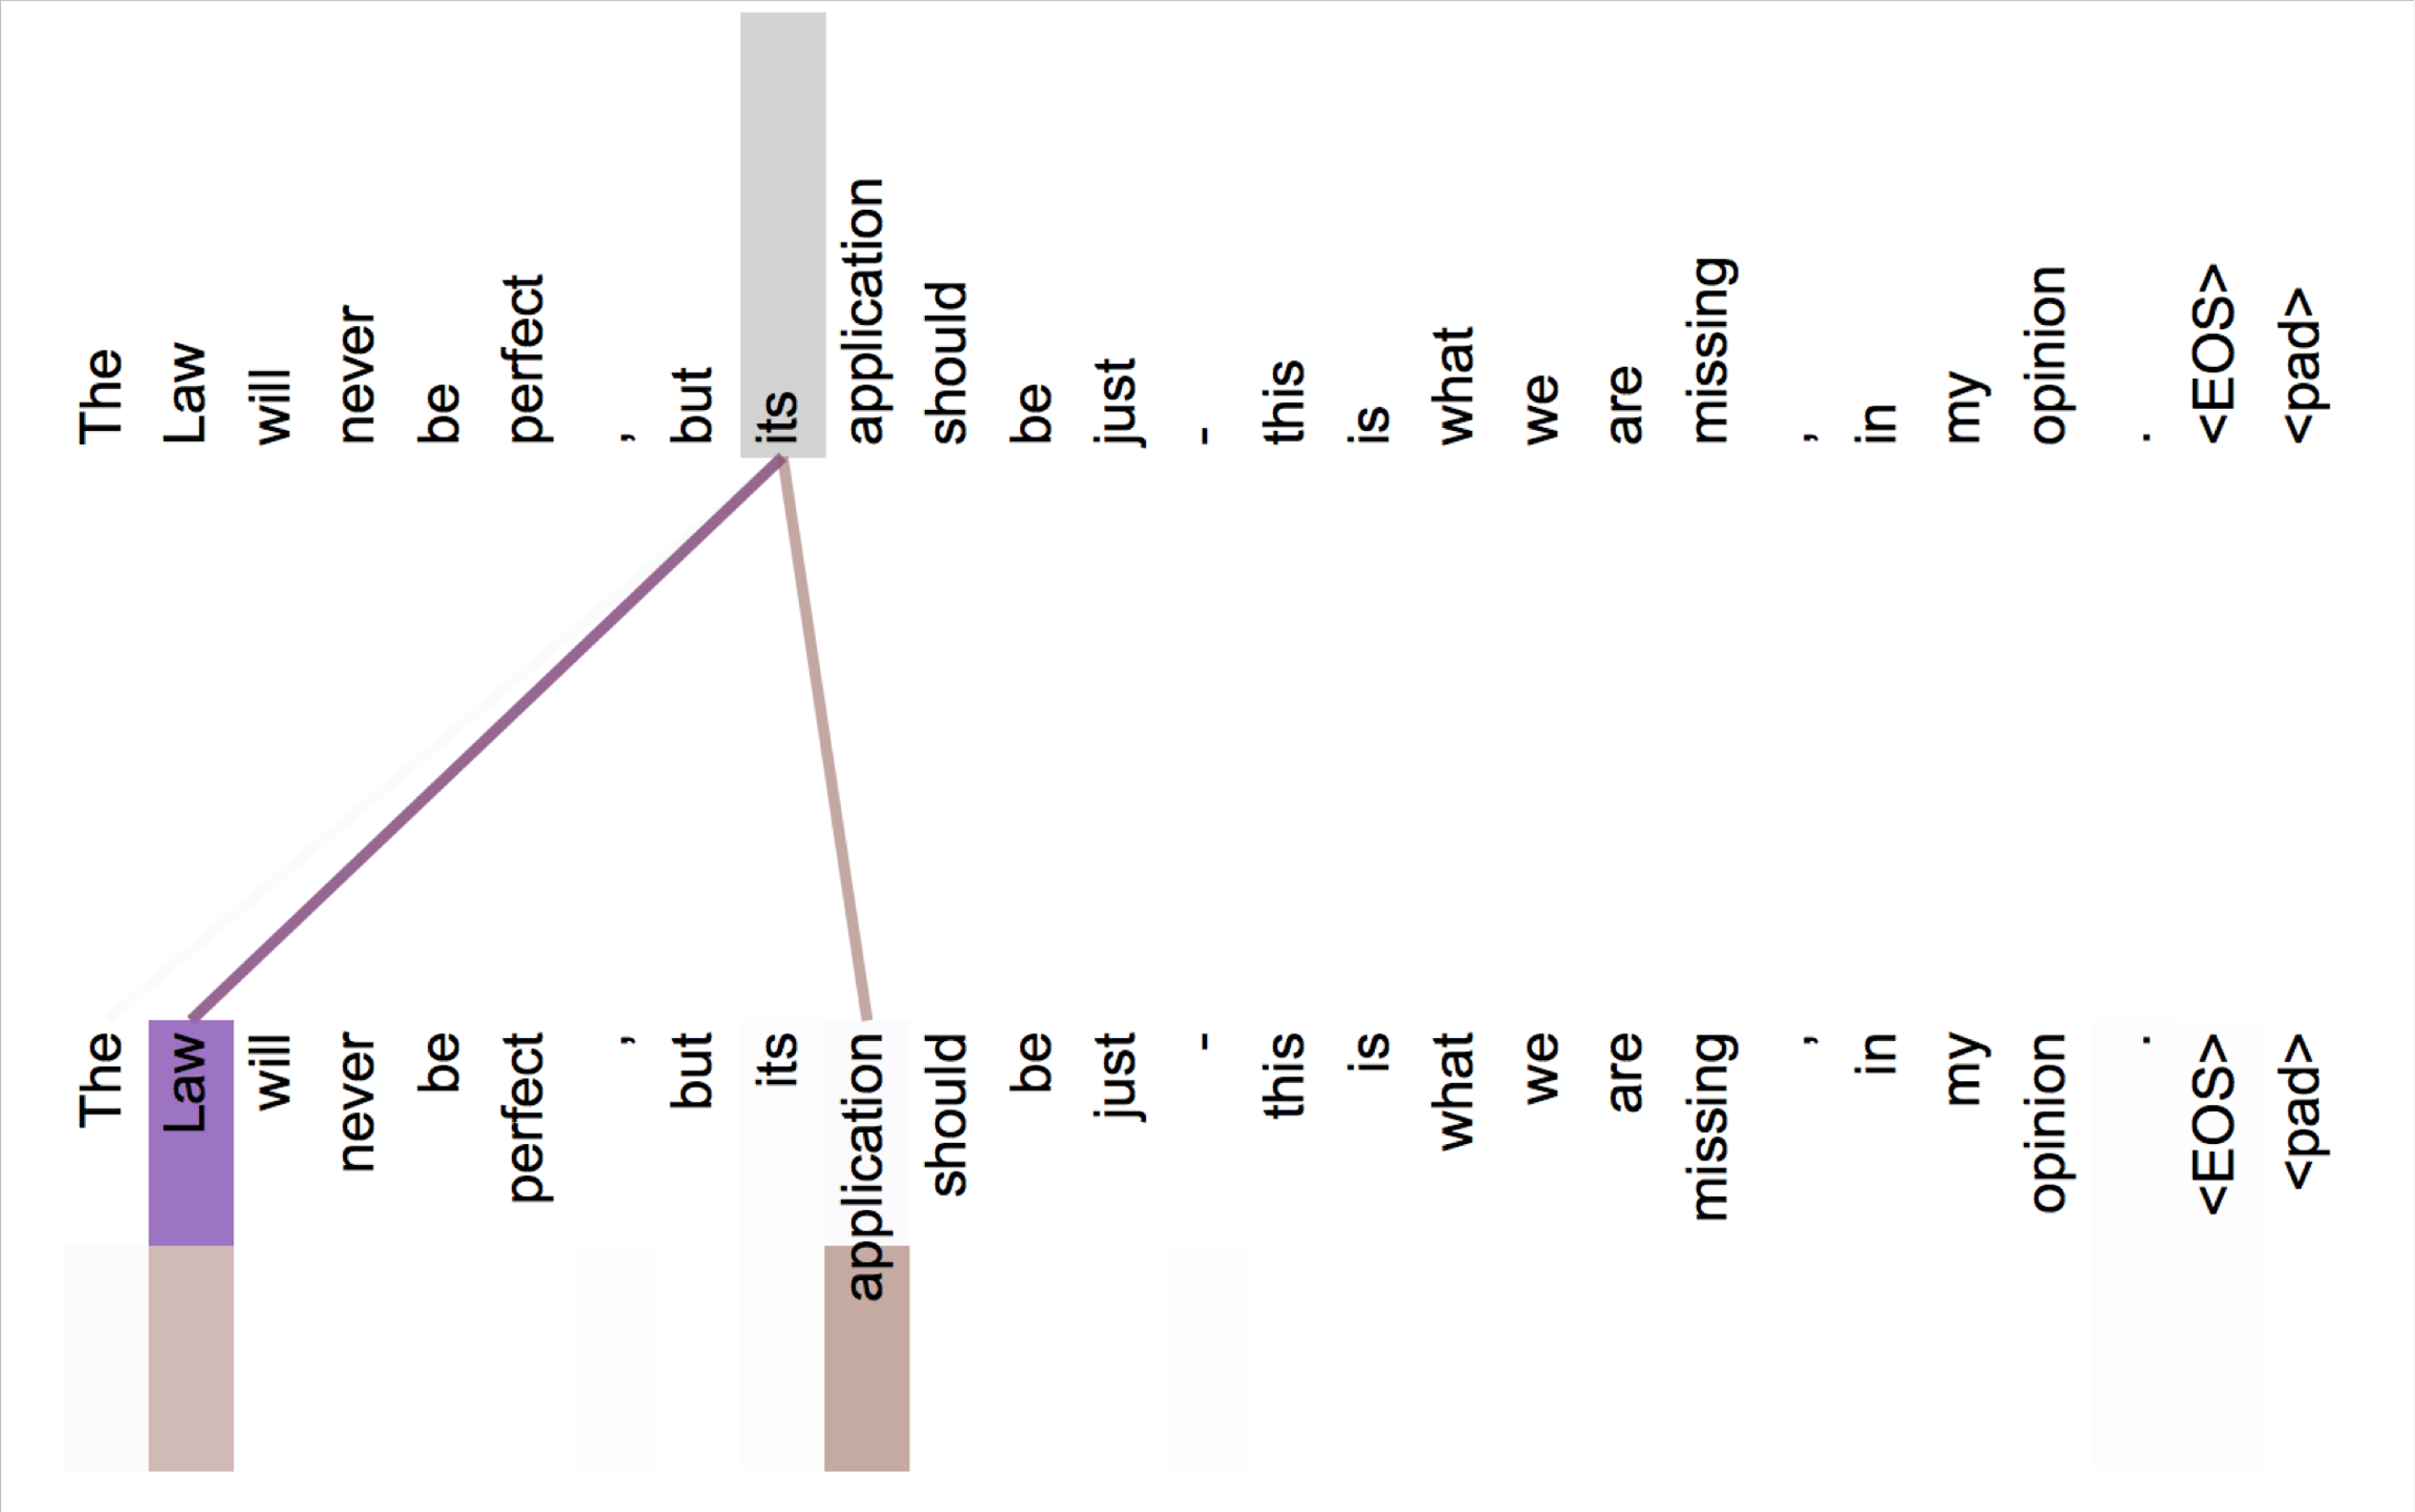
\includegraphics[width=0.6\linewidth,keepaspectratio]{bert80}
			% \end{center}		
			
			% In 5th layer. Isolated attentions from just the word ‘its’ for attention heads 5 and 6.  Note that the attentions are very sharp for this word.

			
			% % {\tiny (Ref: CS224n: Natural Language Processing with Deep Learning - Christopher Manning)}

% \end{frame}

% %%%%%%%%%%%%%%%%%%%%%%%%%%%%%%%%%%%%%%%%%%%%%%%%%%%%%%%%%%%
% \begin{frame}[fragile]\frametitle{Parallel attention heads}

			
			% \begin{center}
			% 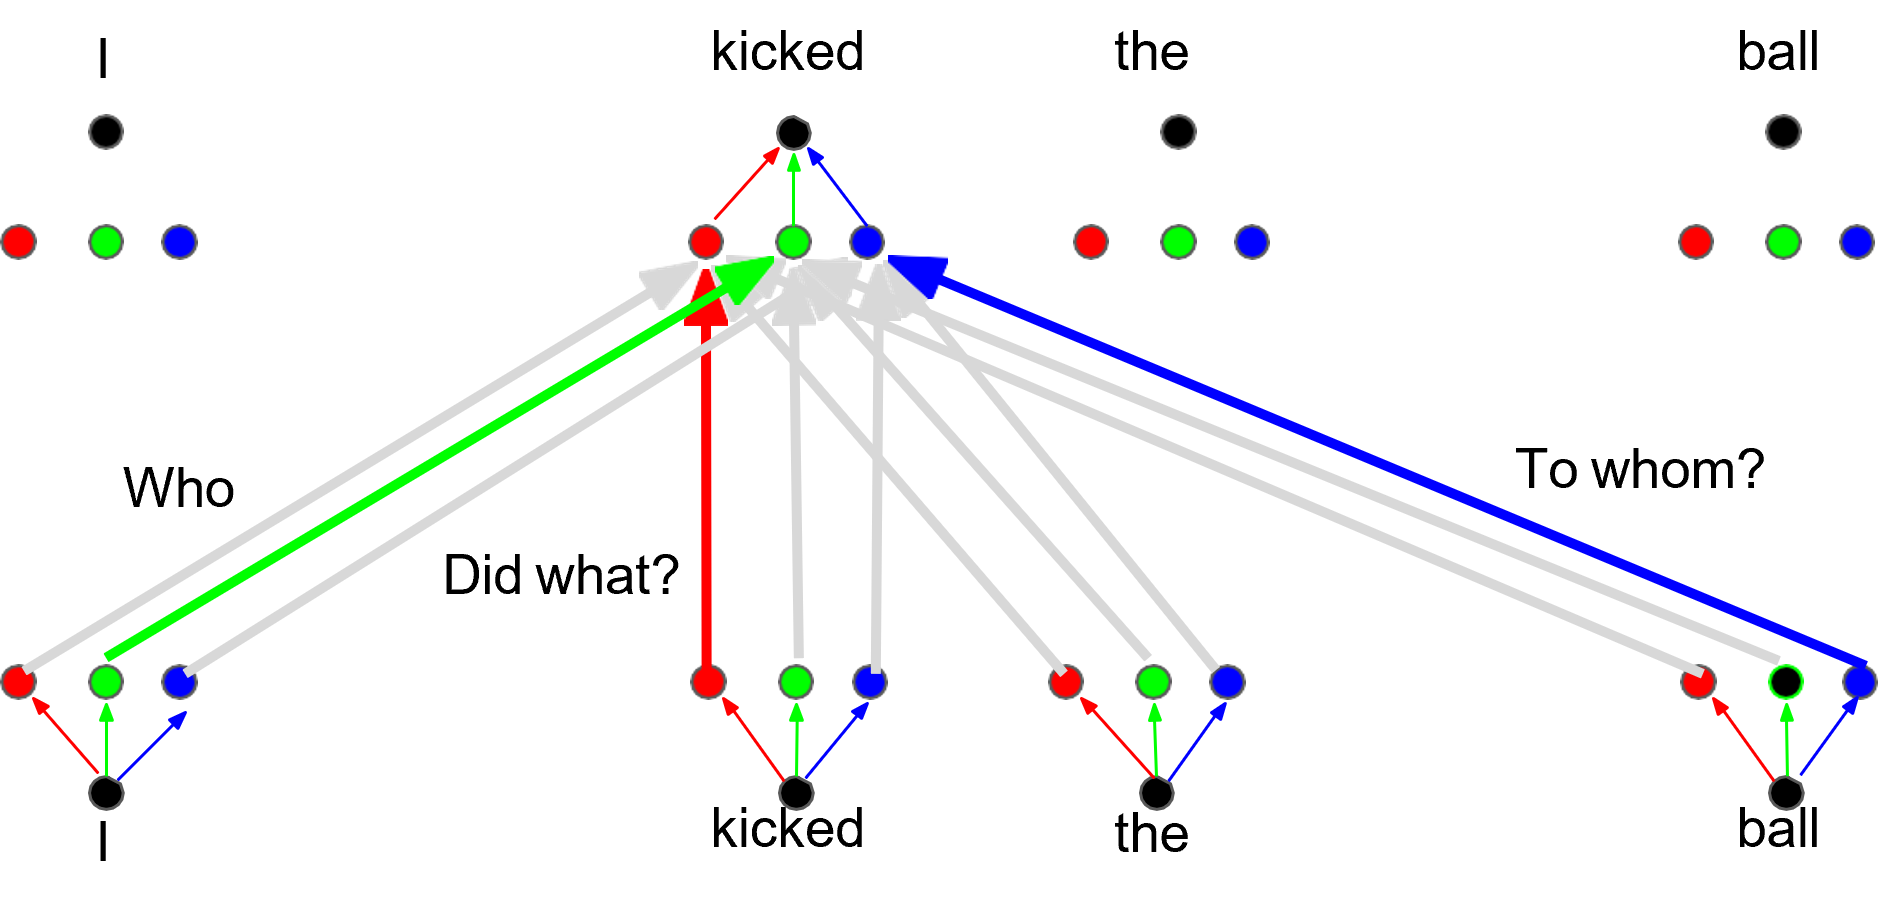
\includegraphics[width=0.6\linewidth,keepaspectratio]{bert81}
			% \end{center}		
			
		
			% % {\tiny (Ref: Ashish Vaswani)}

% \end{frame}

%%%%%%%%%%%%%%%%%%%%%%%%%%%%%%%%%%%%%%%%%%%%%%%%%%%%%%%%%%%%%%%%%%%%%%%%%%%%%%%%%%
\begin{frame}[fragile]\frametitle{}
\begin{center}
{\Large Add \& Norm}
\end{center}
\end{frame}

%%%%%%%%%%%%%%%%%%%%%%%%%%%%%%%%%%%%%%%%%%%%%%%%%%%%%%%%%%%%%%%%%%%%%%%%%%%%%%%%%%
\begin{frame}[fragile]\frametitle{}
\begin{center}
{\Large Feed Forward}
\end{center}
\end{frame}

% %%%%%%%%%%%%%%%%%%%%%%%%%%%%%%%%%%%%%%%%%%%%%%%%%%%%%%%%%%%
% \begin{frame}[fragile]\frametitle{Residual connections}

			% The Transformer Encoder: Residual connections [He et al., 2016]
			
			% \begin{center}
			% 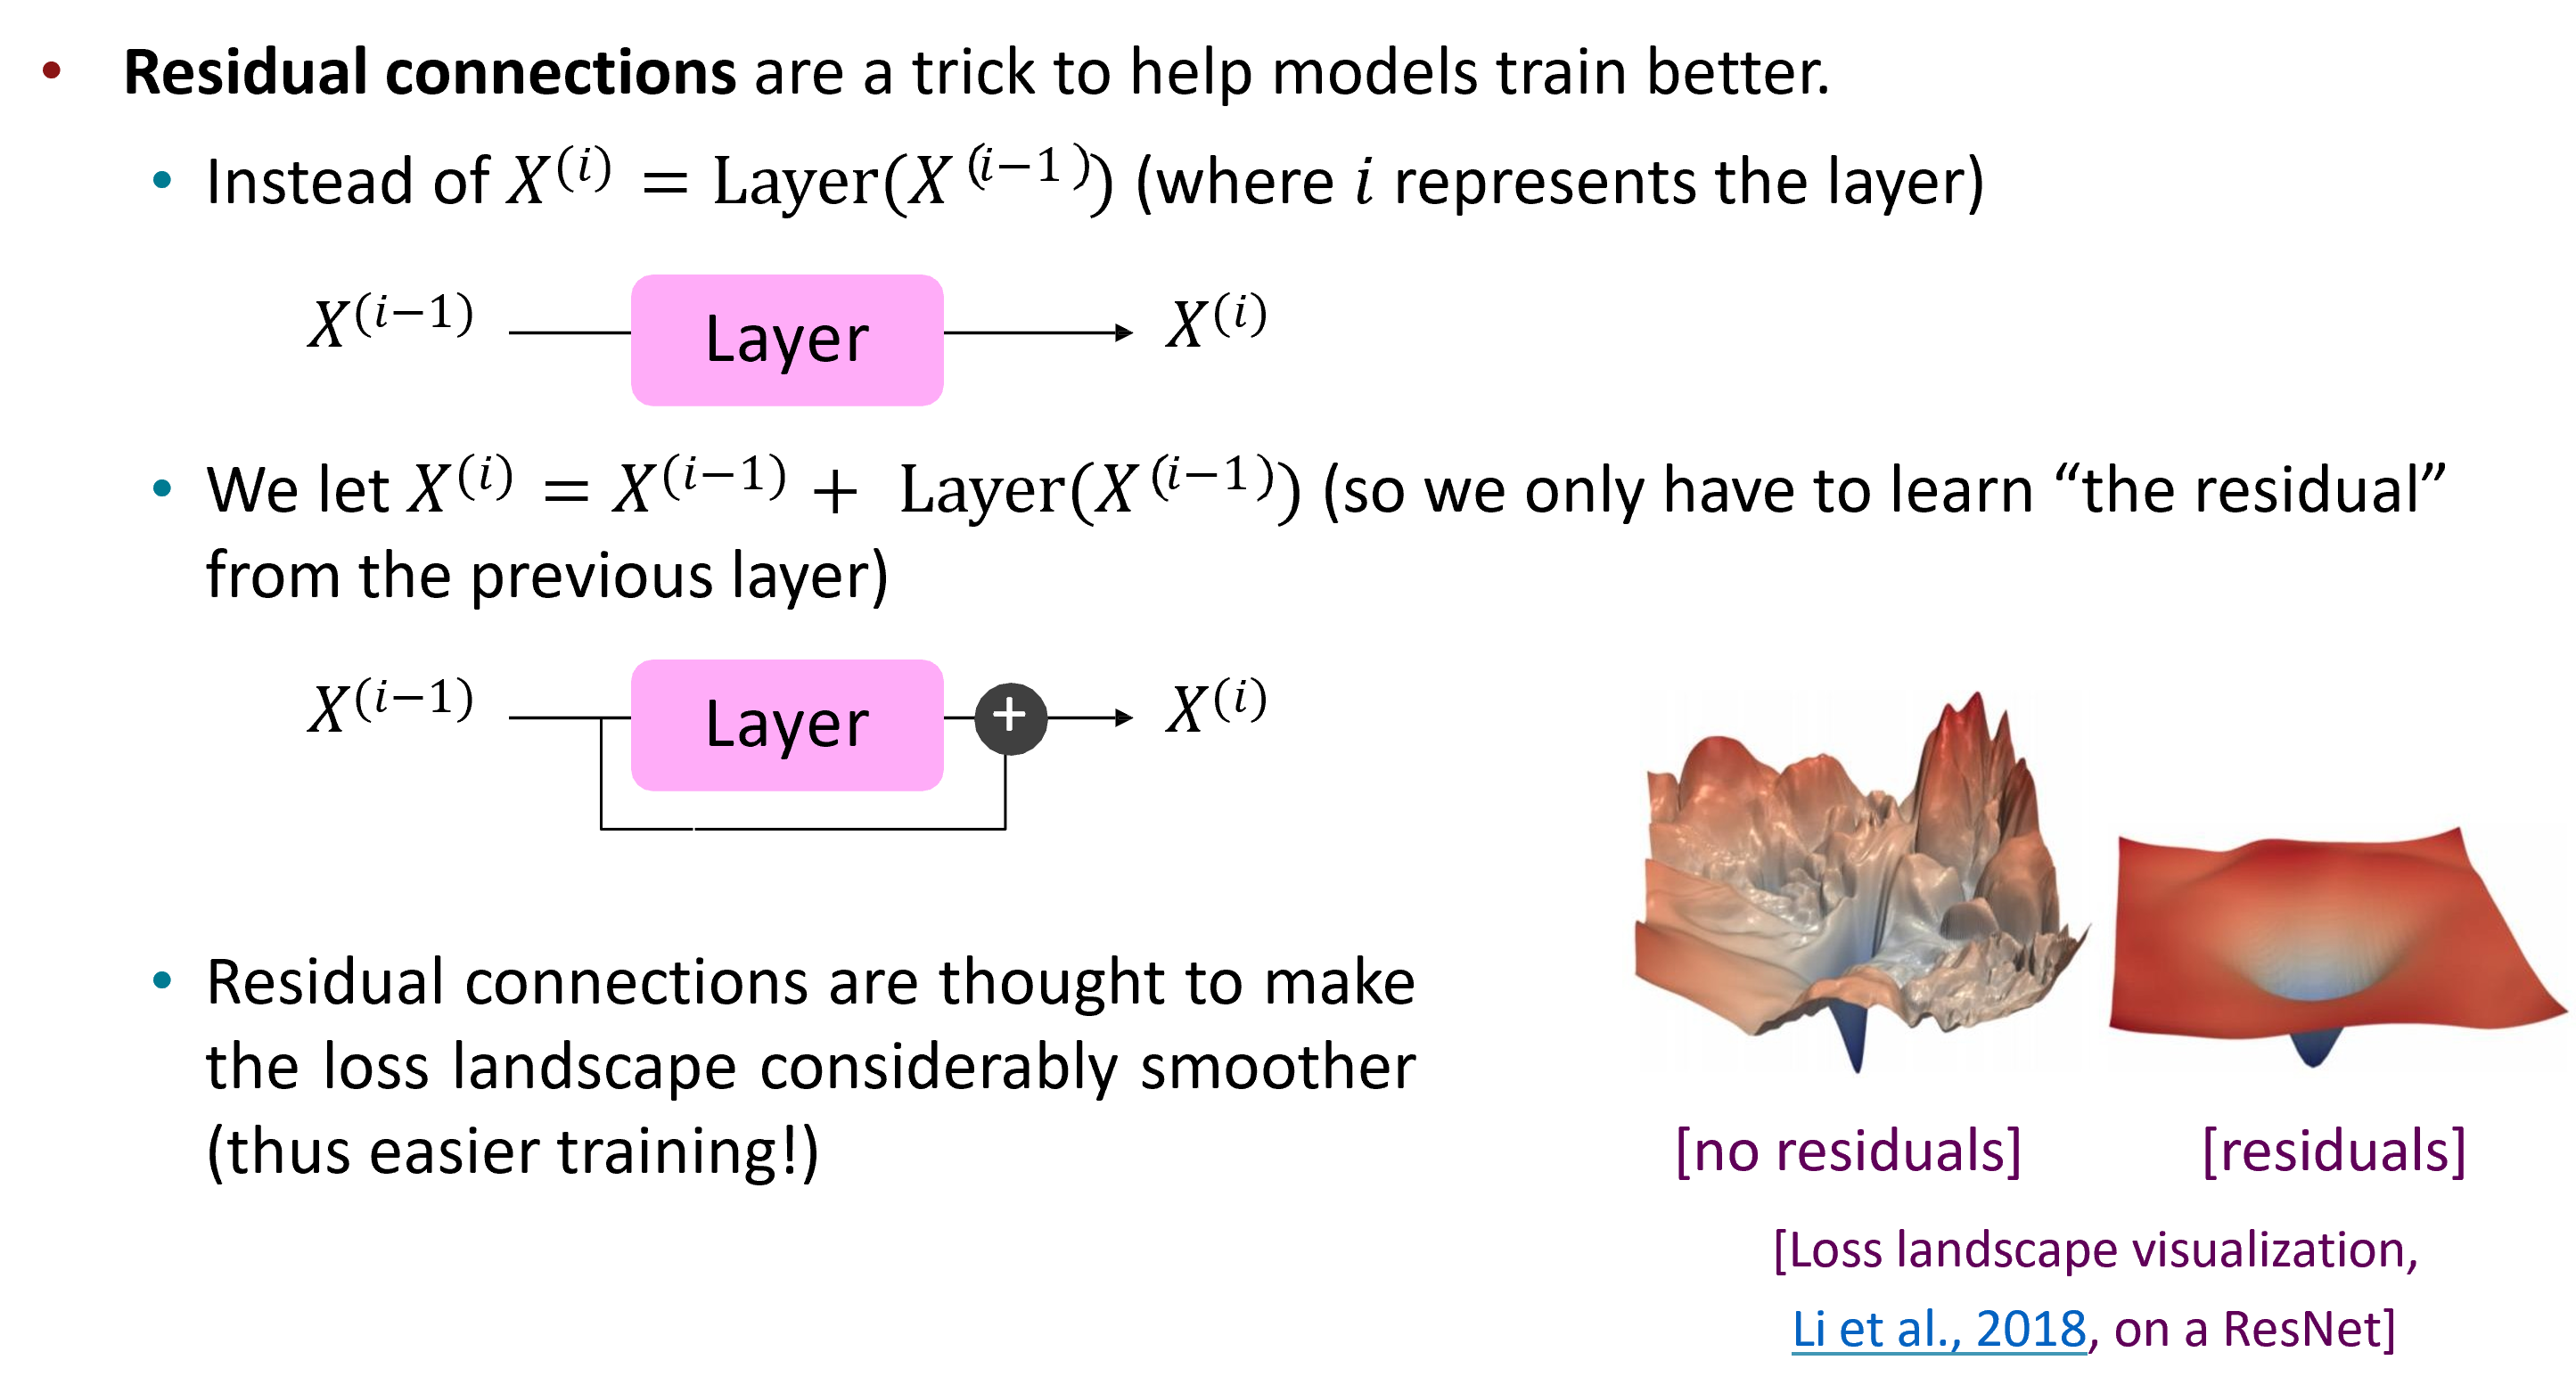
\includegraphics[width=\linewidth,keepaspectratio]{bert82}
			% \end{center}		
			
		
			% % {\tiny (Ref: John Hewitt)}

% \end{frame}

% %%%%%%%%%%%%%%%%%%%%%%%%%%%%%%%%%%%%%%%%%%%%%%%%%%%%%%%%%%%
% \begin{frame}[fragile]\frametitle{Layer normalization}
% The Transformer Encoder: Layer normalization [Ba et al., 2016]
			
			% \begin{center}
			% 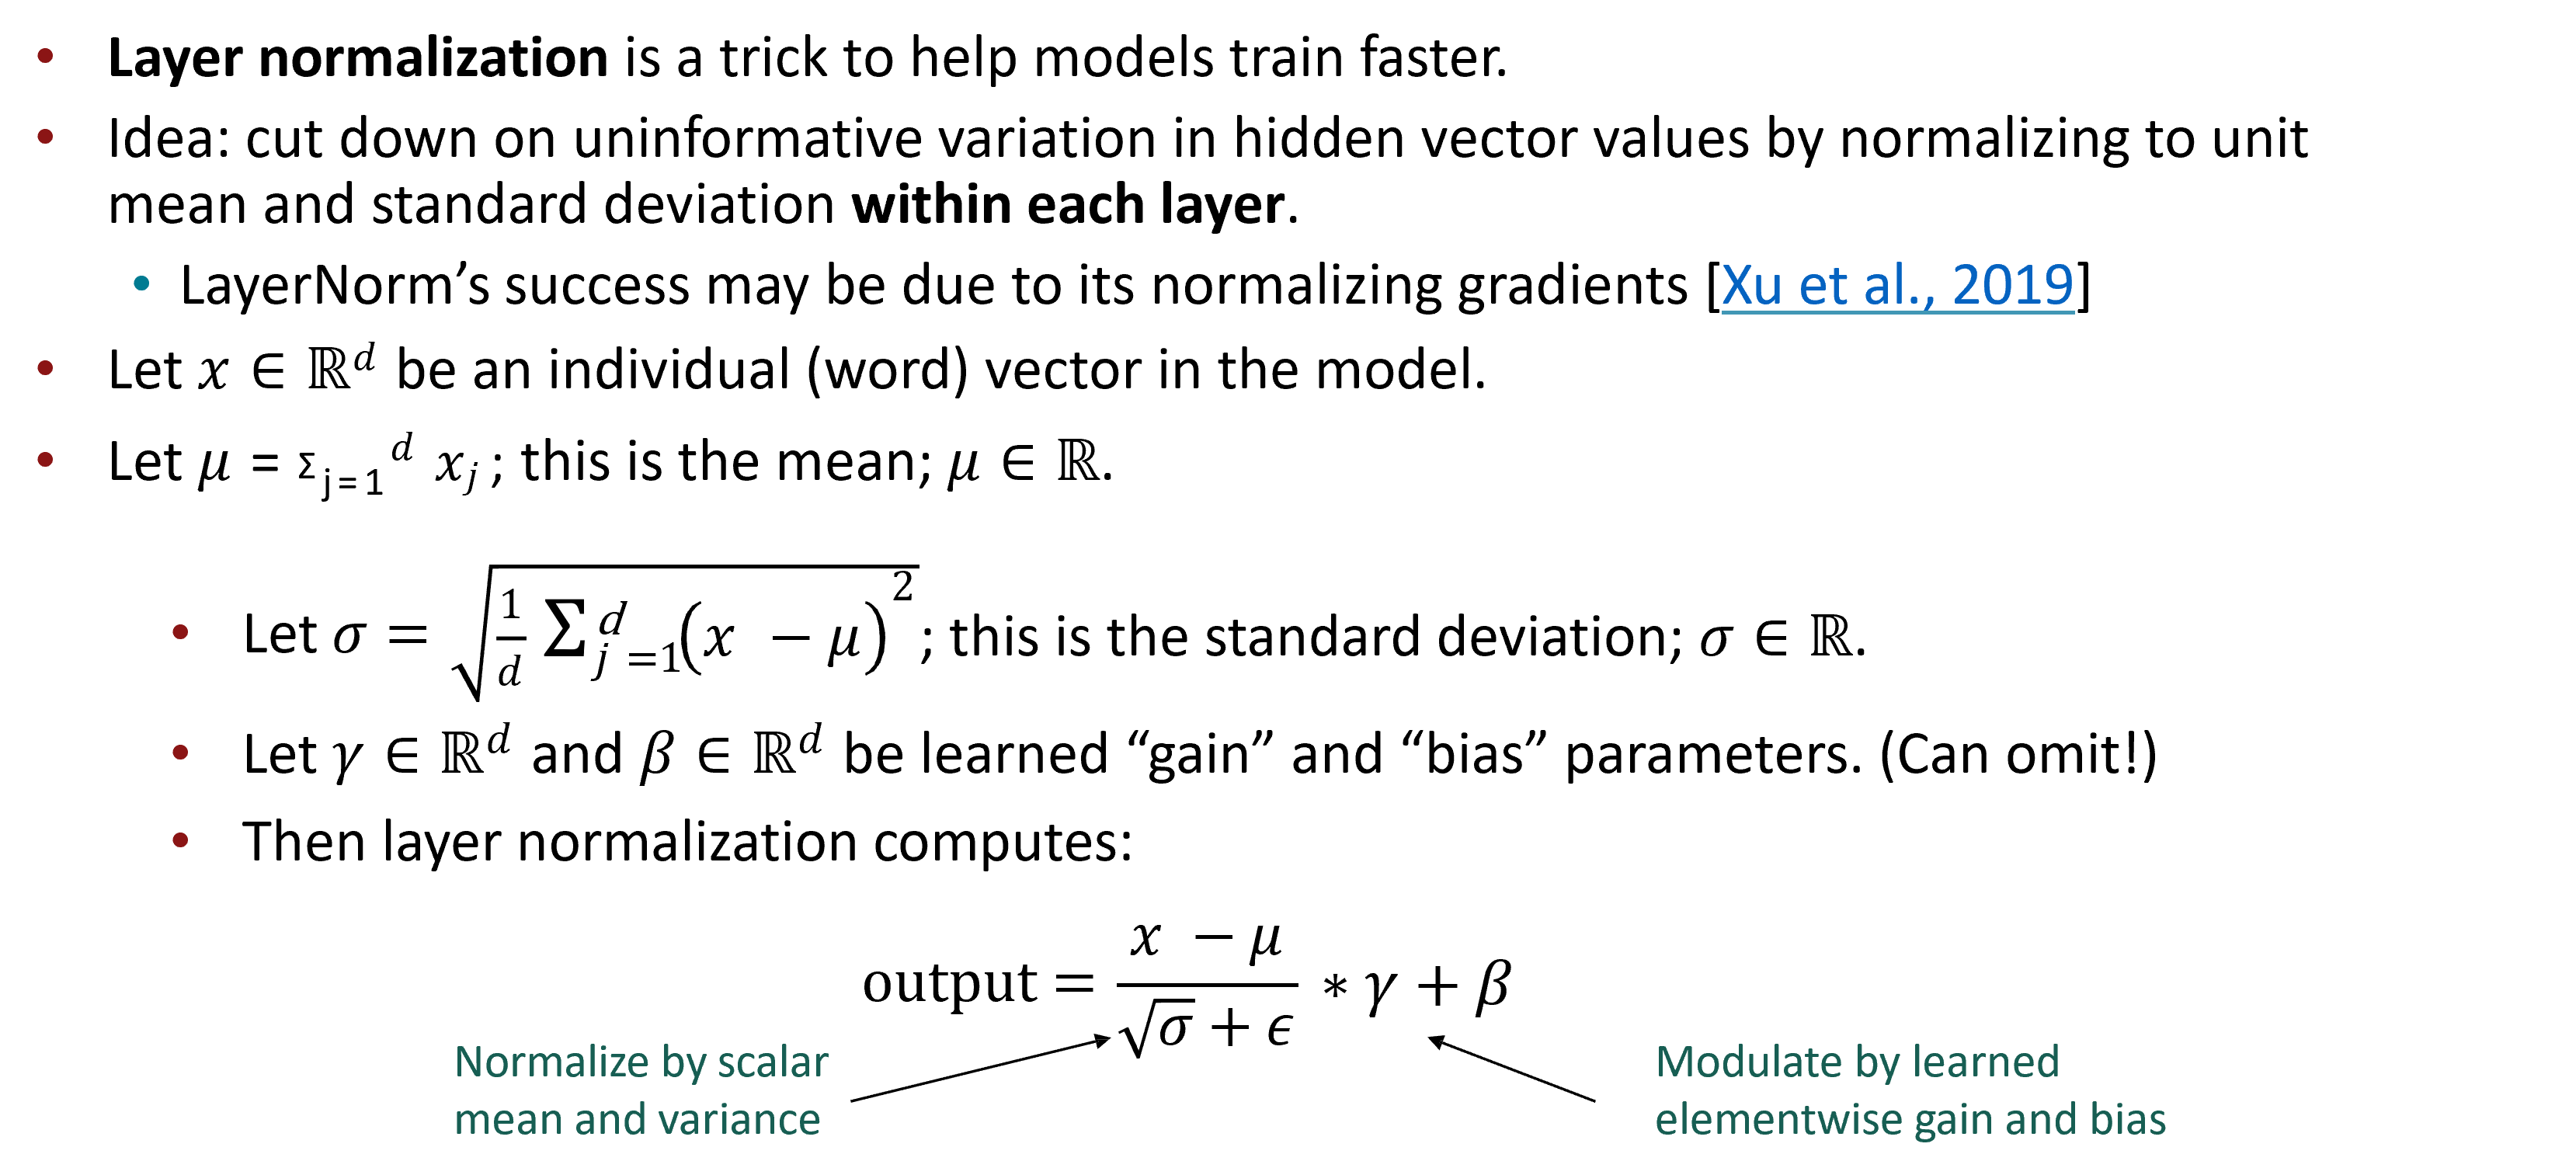
\includegraphics[width=\linewidth,keepaspectratio]{bert83}
			% \end{center}		
			
		
			% % {\tiny (Ref: John Hewitt)}

% \end{frame}

% %%%%%%%%%%%%%%%%%%%%%%%%%%%%%%%%%%%%%%%%%%%%%%%%%%%%%%%%%%%
% \begin{frame}[fragile]\frametitle{ Softmax}

			% The Transformer Encoder: Scaled Dot Product [Vaswani et al., 2017]
			% \begin{center}
			% 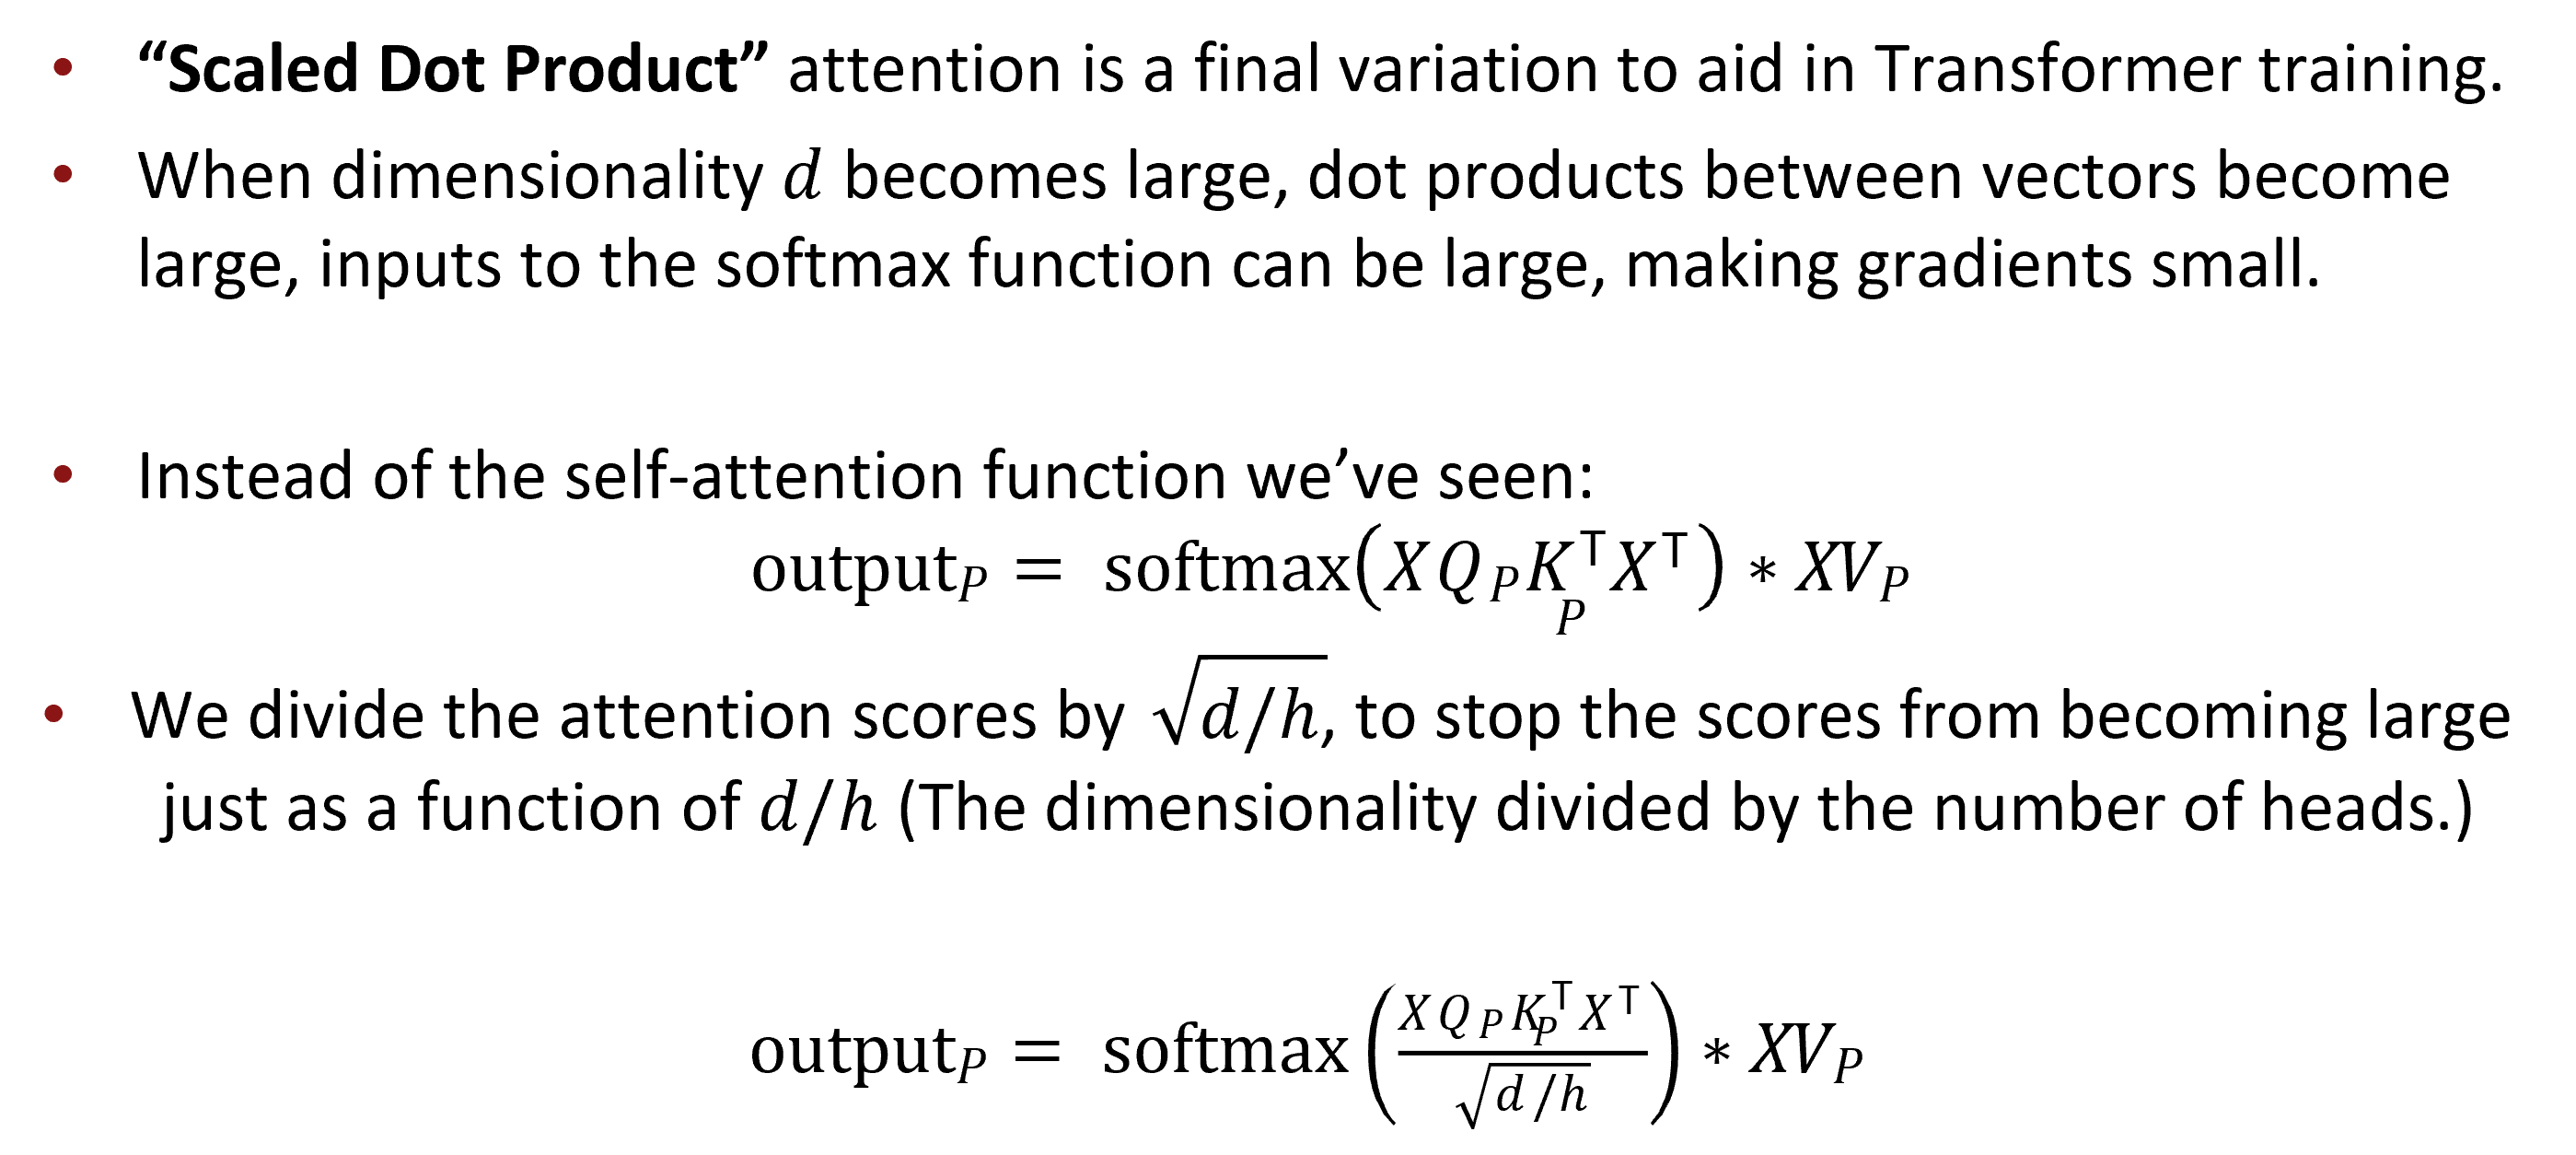
\includegraphics[width=\linewidth,keepaspectratio]{bert84}
			% \end{center}		
			
		
			% % {\tiny (Ref: John Hewitt)}

% \end{frame}

%%%%%%%%%%%%%%%%%%%%%%%%%%%%%%%%%%%%%%%%%%%%%%%%%%%%%%%%%%%%%%%%%%%%%%%%%%%%%%%%%%
\begin{frame}[fragile]\frametitle{}
\begin{center}
{\Large Encoder side is ready with latent space, parallel word embedding of the input sentence ie BERT}
\end{center}
\end{frame}



%%%%%%%%%%%%%%%%%%%%%%%%%%%%%%%%%%%%%%%%%%%%%%%%%%%%%%%%%%%%%%%%%%%%%%%%%%%%%%%%%%
\begin{frame}[fragile]\frametitle{}
\begin{center}
{\Large Decoder Side}
\end{center}
\end{frame}

%%%%%%%%%%%%%%%%%%%%%%%%%%%%%%%%%%%%%%%%%%%%%%%%%%%%%%%%%%%%%%%%%%%%%%%%%%%%%%%%%%
\begin{frame}[fragile]\frametitle{}
\begin{center}
{\Large Output Embedding plus Positional Encoding}
\end{center}
\end{frame}

%%%%%%%%%%%%%%%%%%%%%%%%%%%%%%%%%%%%%%%%%%%%%%%%%%%%%%%%%%%%%%%%%%%%%%%%%%%%%%%%%%
\begin{frame}[fragile]\frametitle{}
\begin{center}
{\Large Masked Attention}
\end{center}
\end{frame}

%%%%%%%%%%%%%%%%%%%%%%%%%%%%%%%%%%%%%%%%%%%%%%%%%%%%%%%%%%%%%%%%%%%%%%%%%%%%%%%%%%
\begin{frame}[fragile]\frametitle{}
\begin{center}
{\Large Masked Multi-head Attention}
\end{center}
\end{frame}


%%%%%%%%%%%%%%%%%%%%%%%%%%%%%%%%%%%%%%%%%%%%%%%%%%%%%%%%%%%%%%%%%%%%%%%%%%%%%%%%%%
\begin{frame}[fragile]\frametitle{}
\begin{center}
{\Large Linear plus Softmax}
\end{center}
\end{frame}

% %%%%%%%%%%%%%%%%%%%%%%%%%%%%%%%%%%%%%%%%%%%%%%%%%%%%%%%%%%%
% \begin{frame}[fragile]\frametitle{Attending Encoder side}

% The Transformer Encoder: Scaled Dot Product [Vaswani et al., 2017]
			
			% \begin{center}
			% 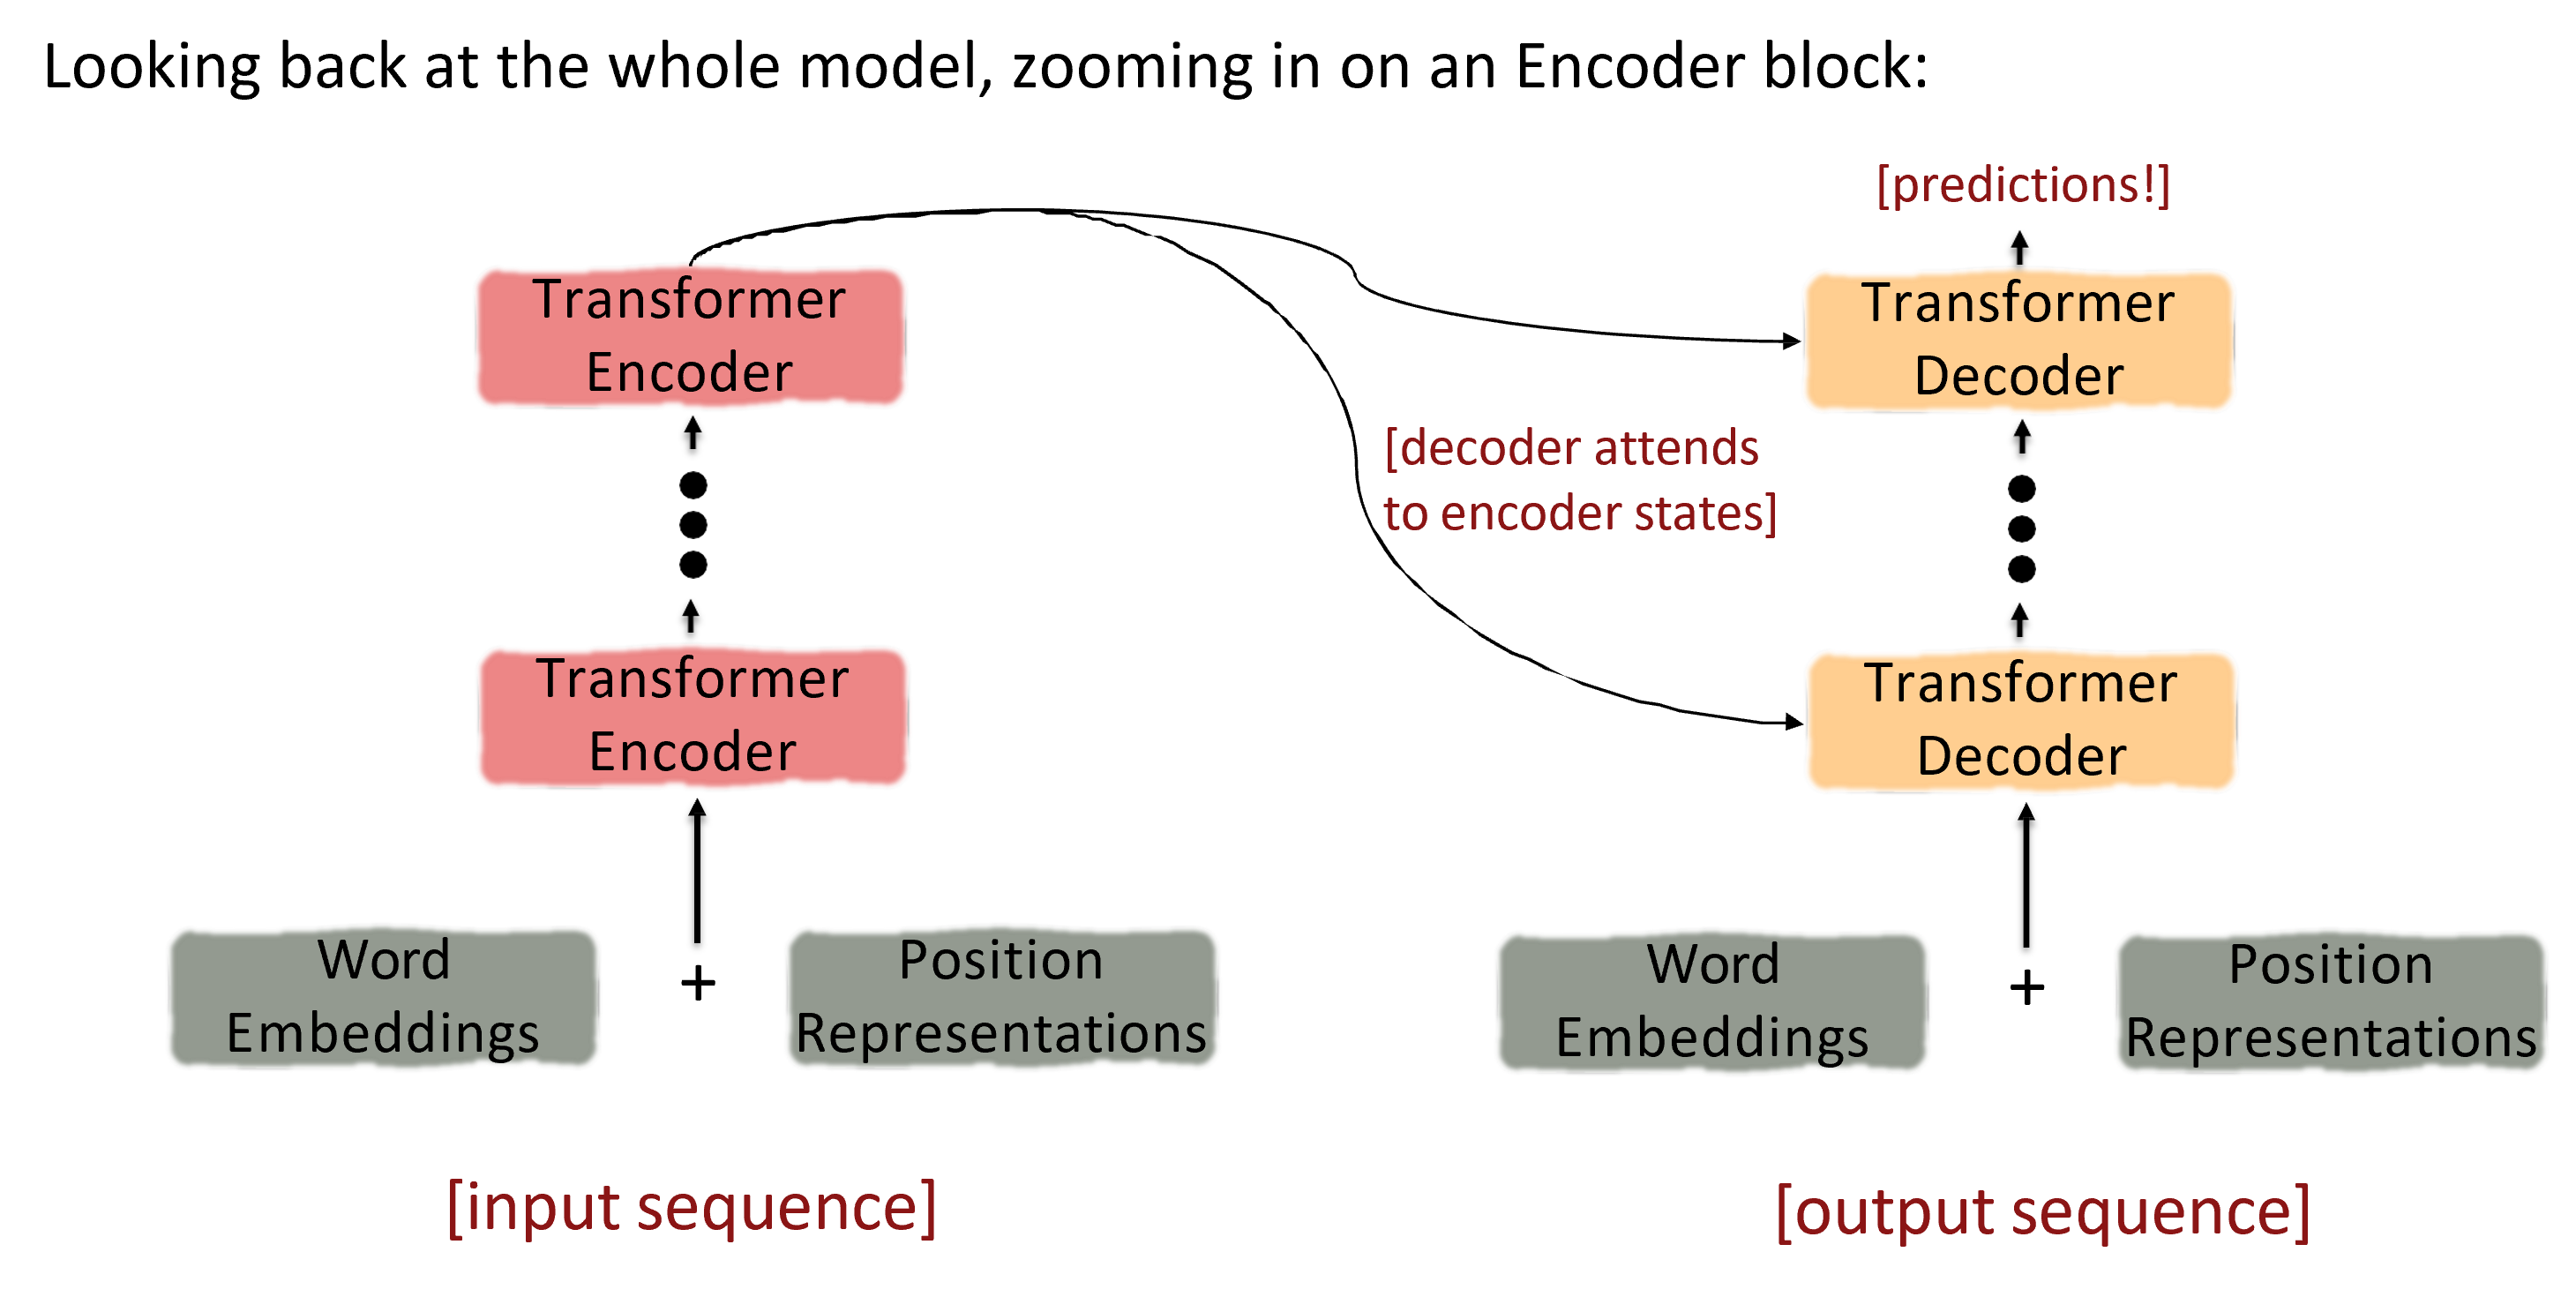
\includegraphics[width=\linewidth,keepaspectratio]{bert85}
			% \end{center}		
			
		
			% % {\tiny (Ref: John Hewitt)}

% \end{frame}

% %%%%%%%%%%%%%%%%%%%%%%%%%%%%%%%%%%%%%%%%%%%%%%%%%%%%%%%%%%%
% \begin{frame}[fragile]\frametitle{Attending Encoder side}

			% The Transformer Encoder: Scaled Dot Product [Vaswani et al., 2017]
			
			% \begin{center}
			% 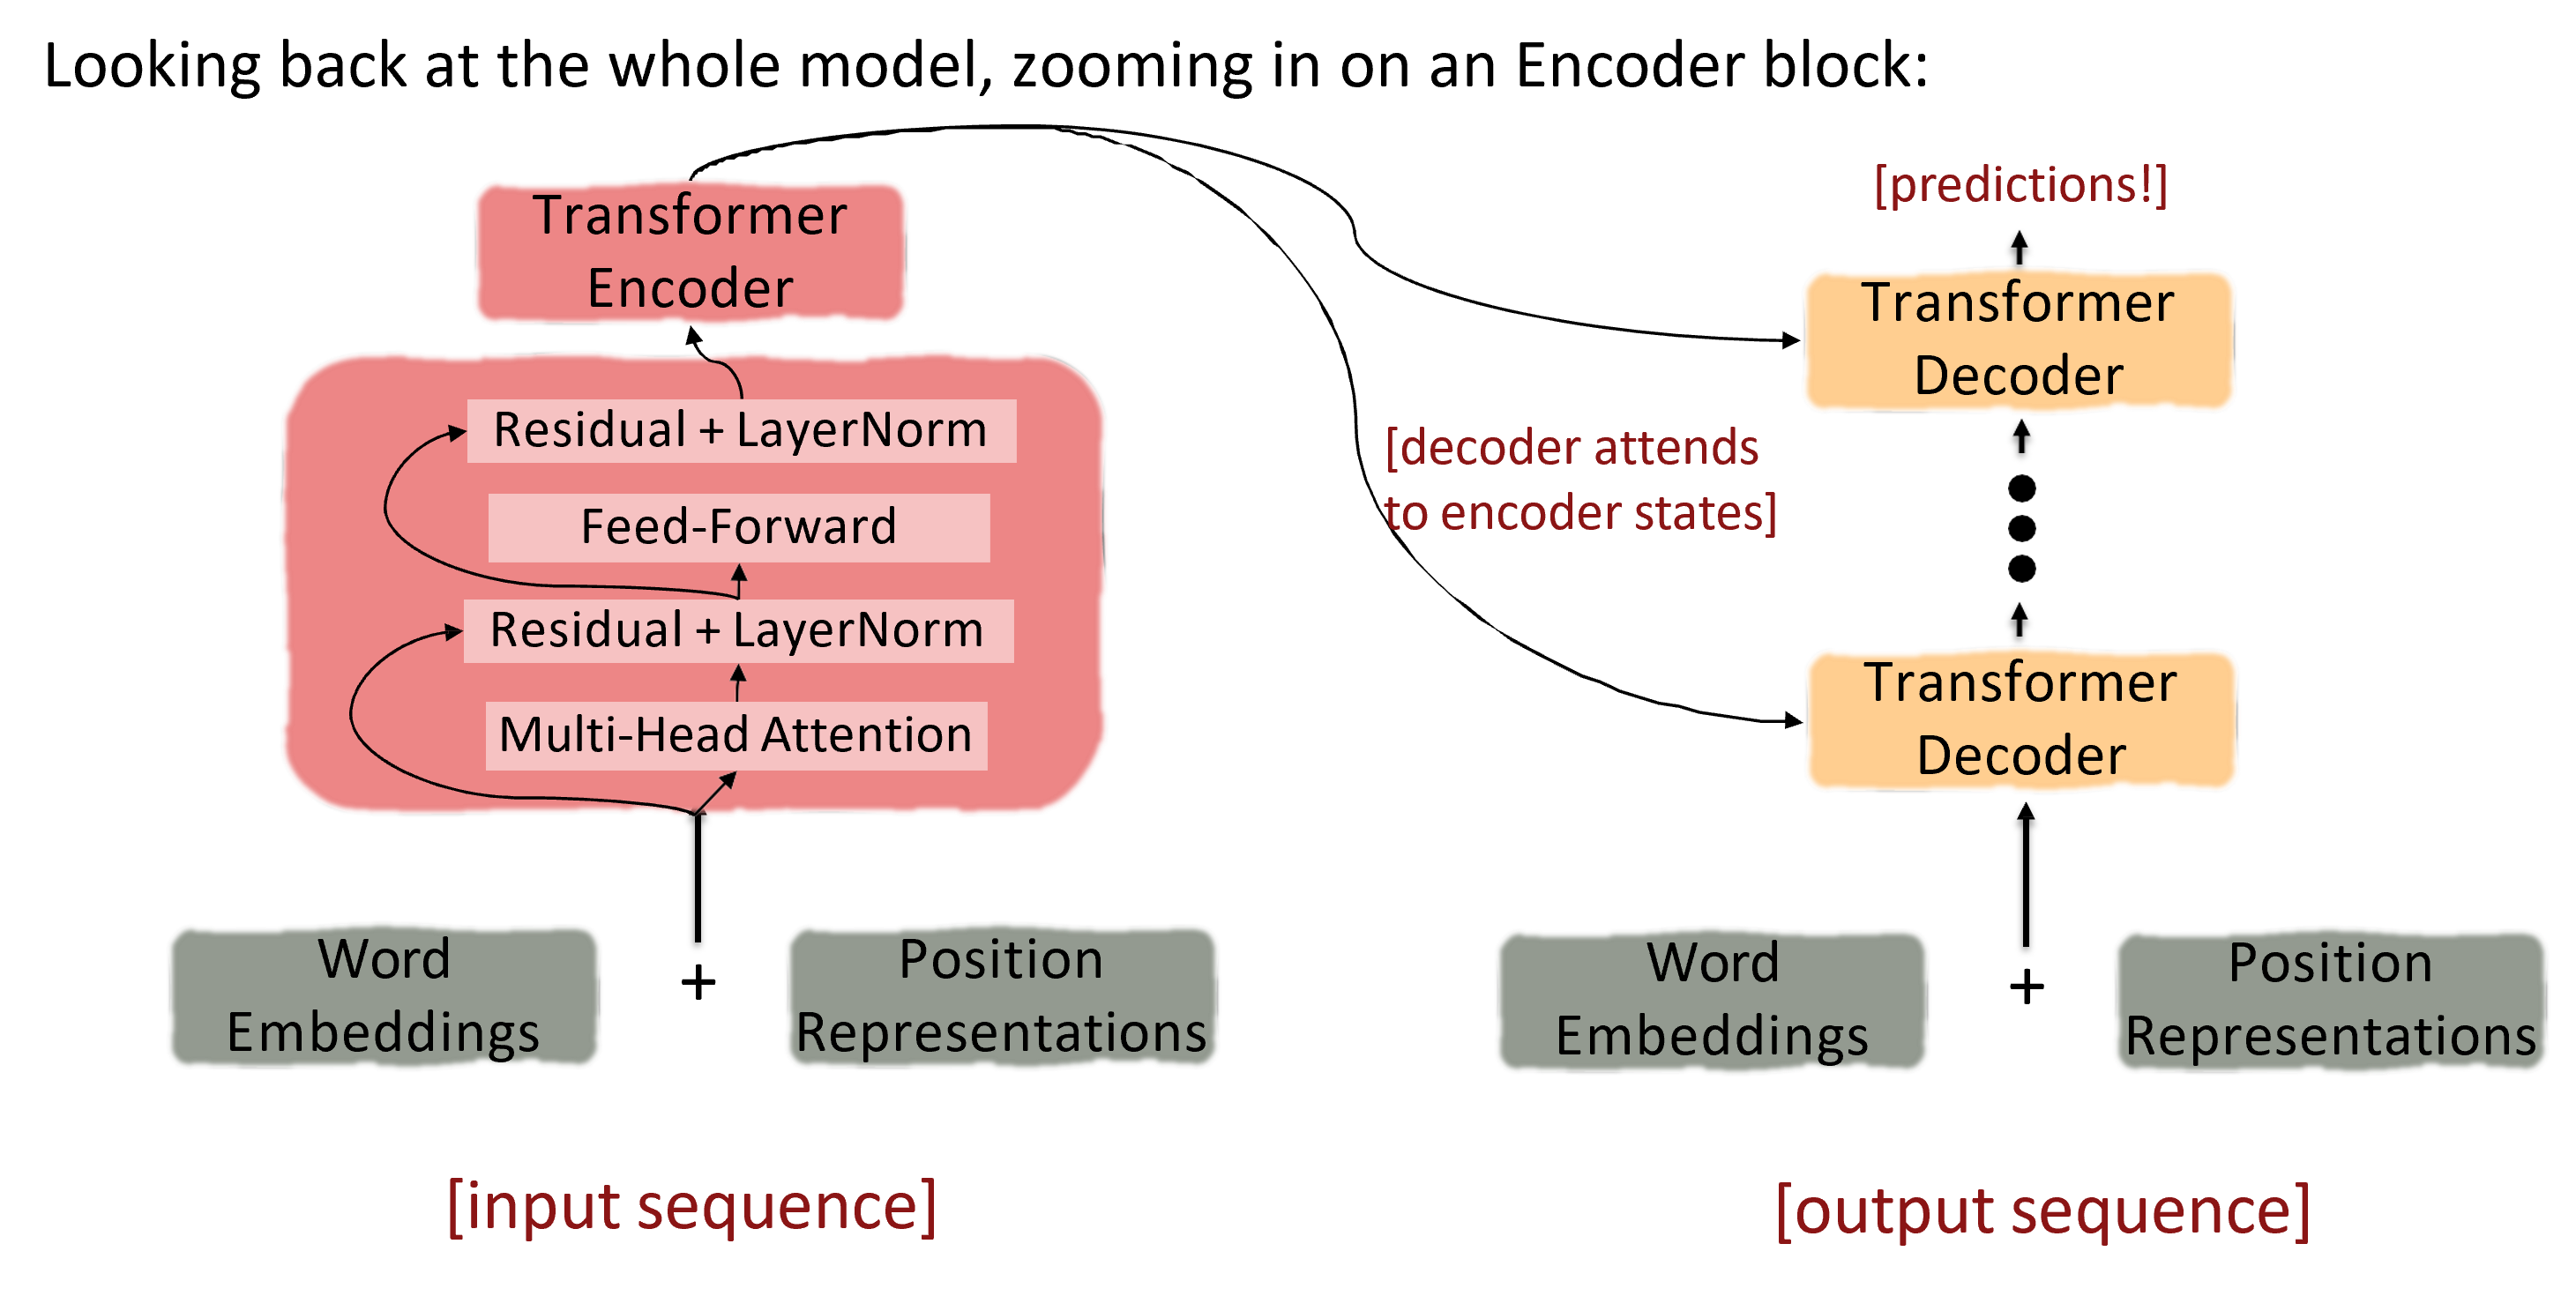
\includegraphics[width=\linewidth,keepaspectratio]{bert86}
			% \end{center}		
			
		
			% % {\tiny (Ref: John Hewitt)}

% \end{frame}

% %%%%%%%%%%%%%%%%%%%%%%%%%%%%%%%%%%%%%%%%%%%%%%%%%%%%%%%%%%%
% \begin{frame}[fragile]\frametitle{Attending Encoder side}

						% The Transformer Encoder: Scaled Dot Product [Vaswani et al., 2017]

			% \begin{center}
			% 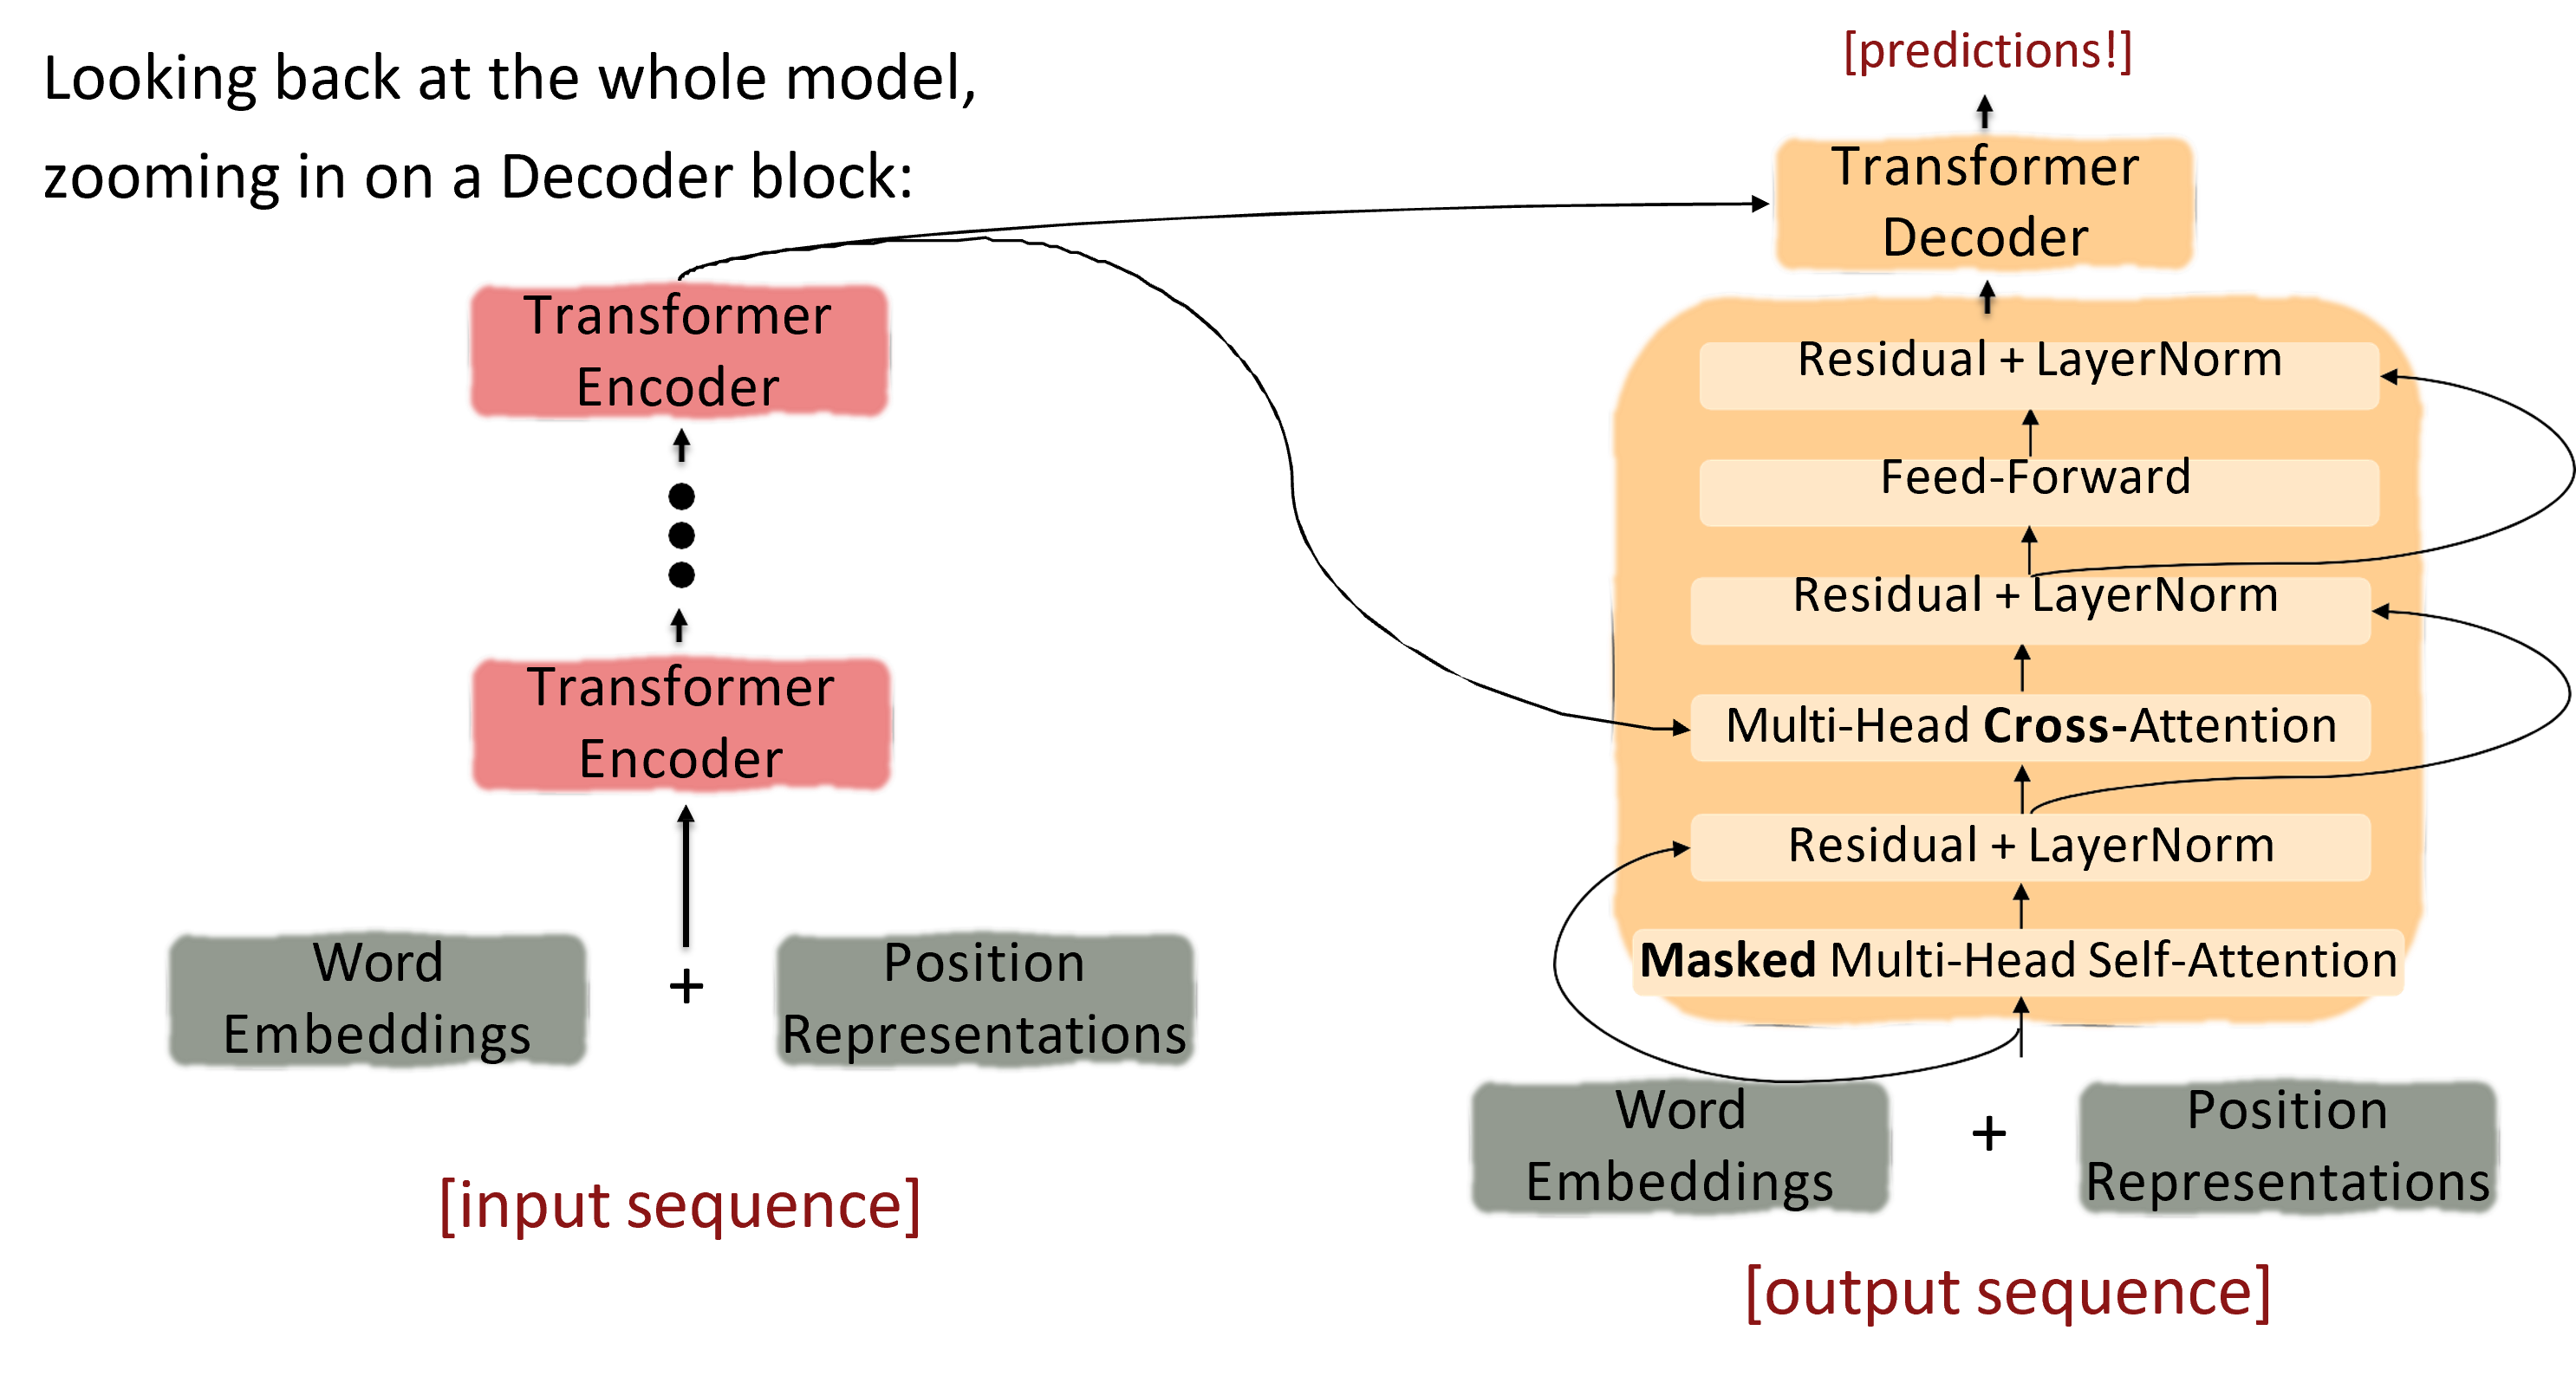
\includegraphics[width=\linewidth,keepaspectratio]{bert87}
			% \end{center}		
			
		
			% % {\tiny (Ref: John Hewitt)}

% \end{frame}

% %%%%%%%%%%%%%%%%%%%%%%%%%%%%%%%%%%%%%%%%%%%%%%%%%%%%%%%%%%%
% \begin{frame}[fragile]\frametitle{Attending Encoder side}

						% The Transformer Encoder: Scaled Dot Product [Vaswani et al., 2017]

			
			% \begin{center}
			% 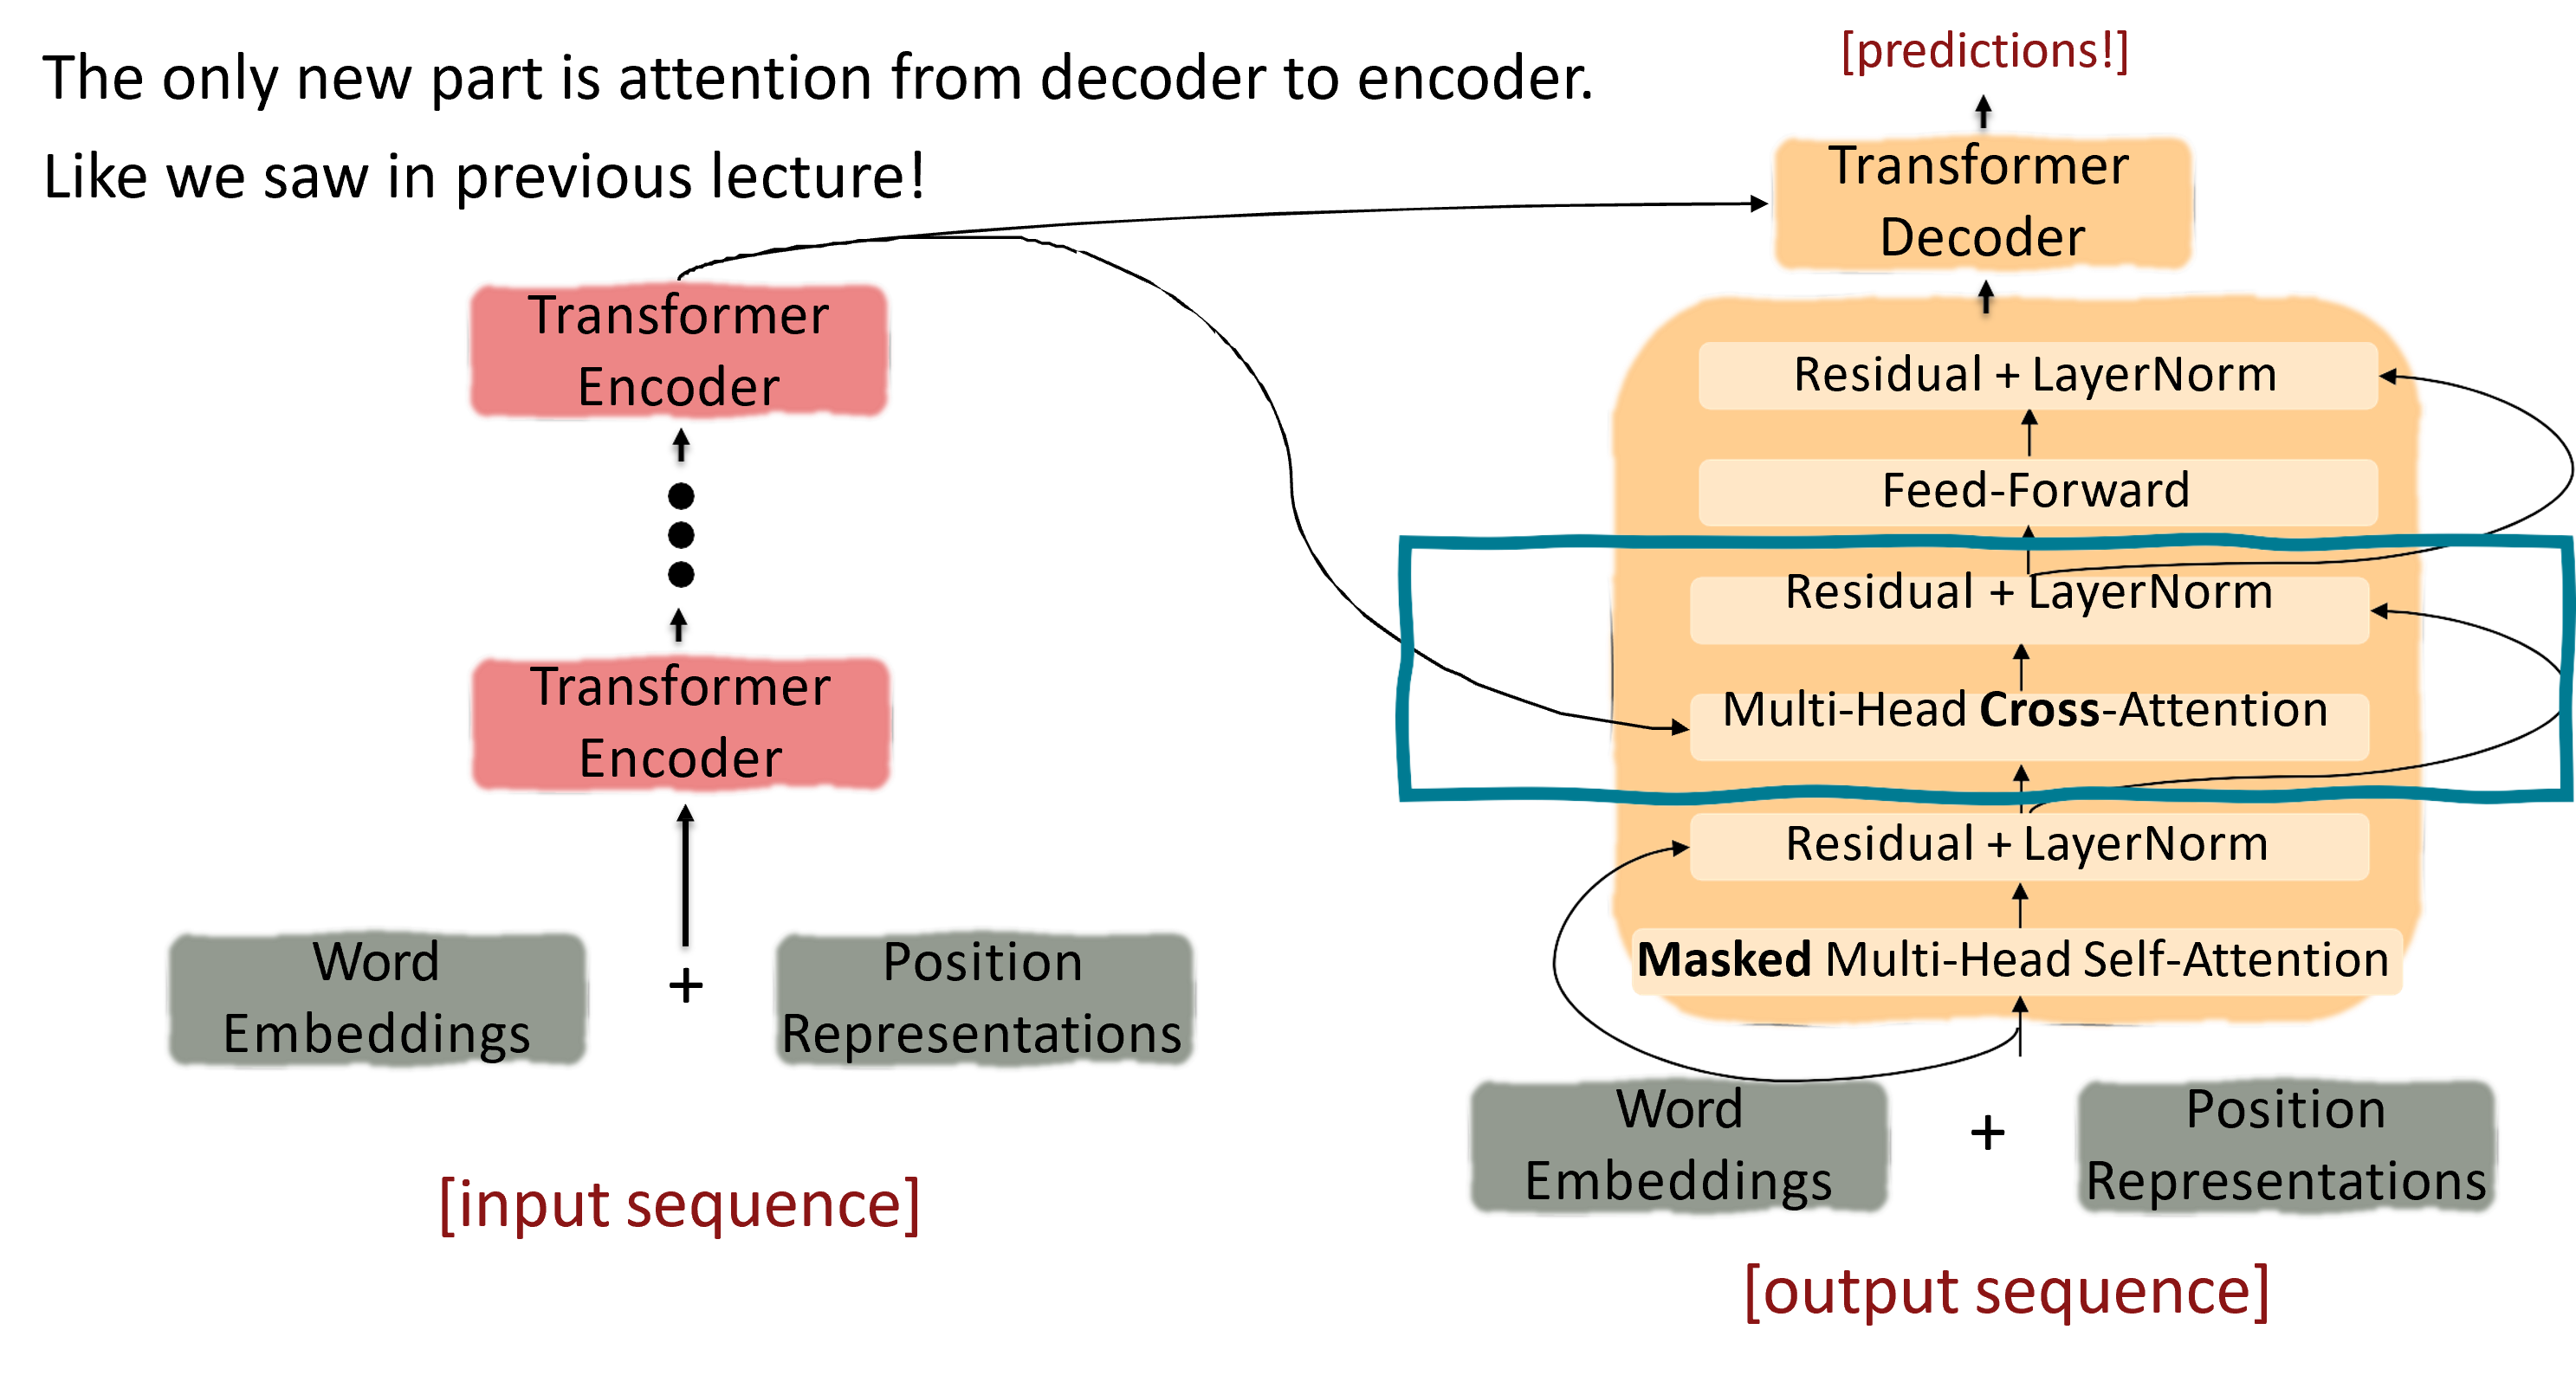
\includegraphics[width=\linewidth,keepaspectratio]{bert88}
			% \end{center}		
			
		
			% % {\tiny (Ref: John Hewitt)}

% \end{frame}

% %%%%%%%%%%%%%%%%%%%%%%%%%%%%%%%%%%%%%%%%%%%%%%%%%%%%%%%%%%%
% \begin{frame}[fragile]\frametitle{Cross-attention}

			% The Transformer Decoder: Cross-attention (details)
			
			% \begin{center}
			% 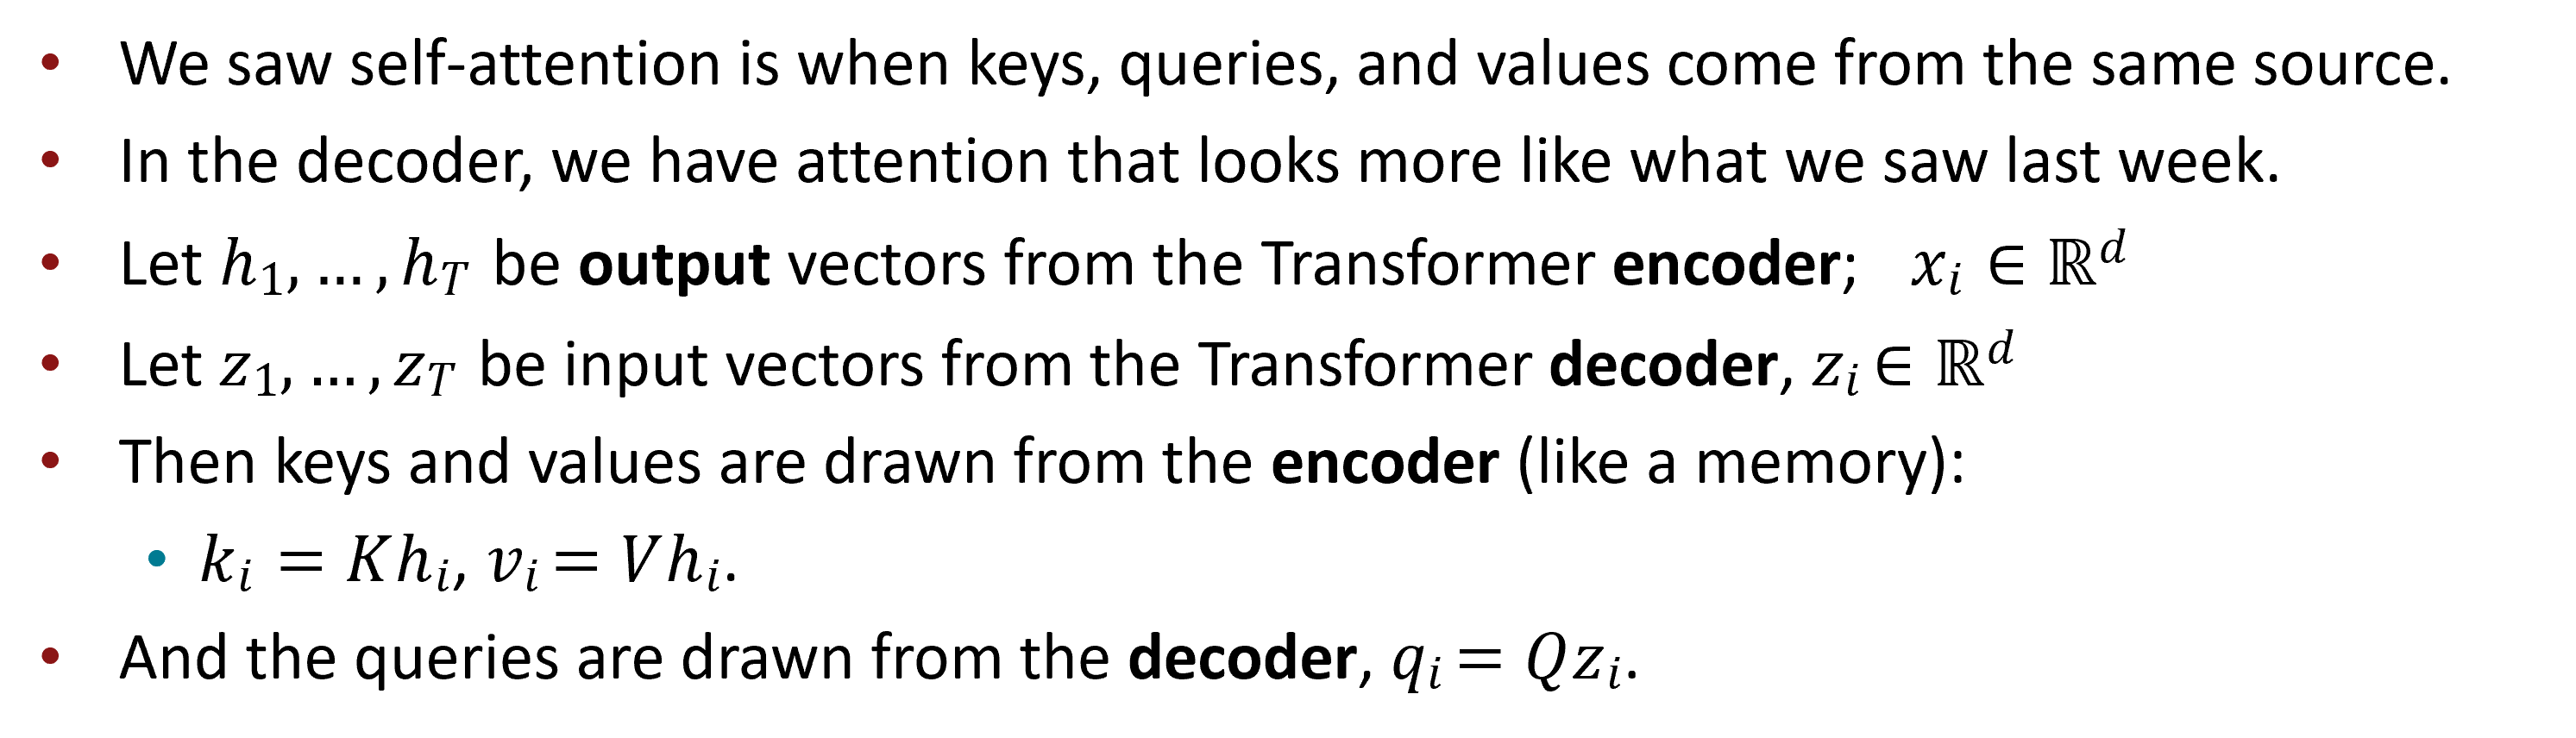
\includegraphics[width=\linewidth,keepaspectratio]{bert89}
			% \end{center}		
			
		
			% % {\tiny (Ref: John Hewitt)}

% \end{frame}

% %%%%%%%%%%%%%%%%%%%%%%%%%%%%%%%%%%%%%%%%%%%%%%%%%%%%%%%%%%%
% \begin{frame}[fragile]\frametitle{Cross-attention}

			% The Transformer Decoder: Cross-attention (details)
			
			% \begin{center}
			% 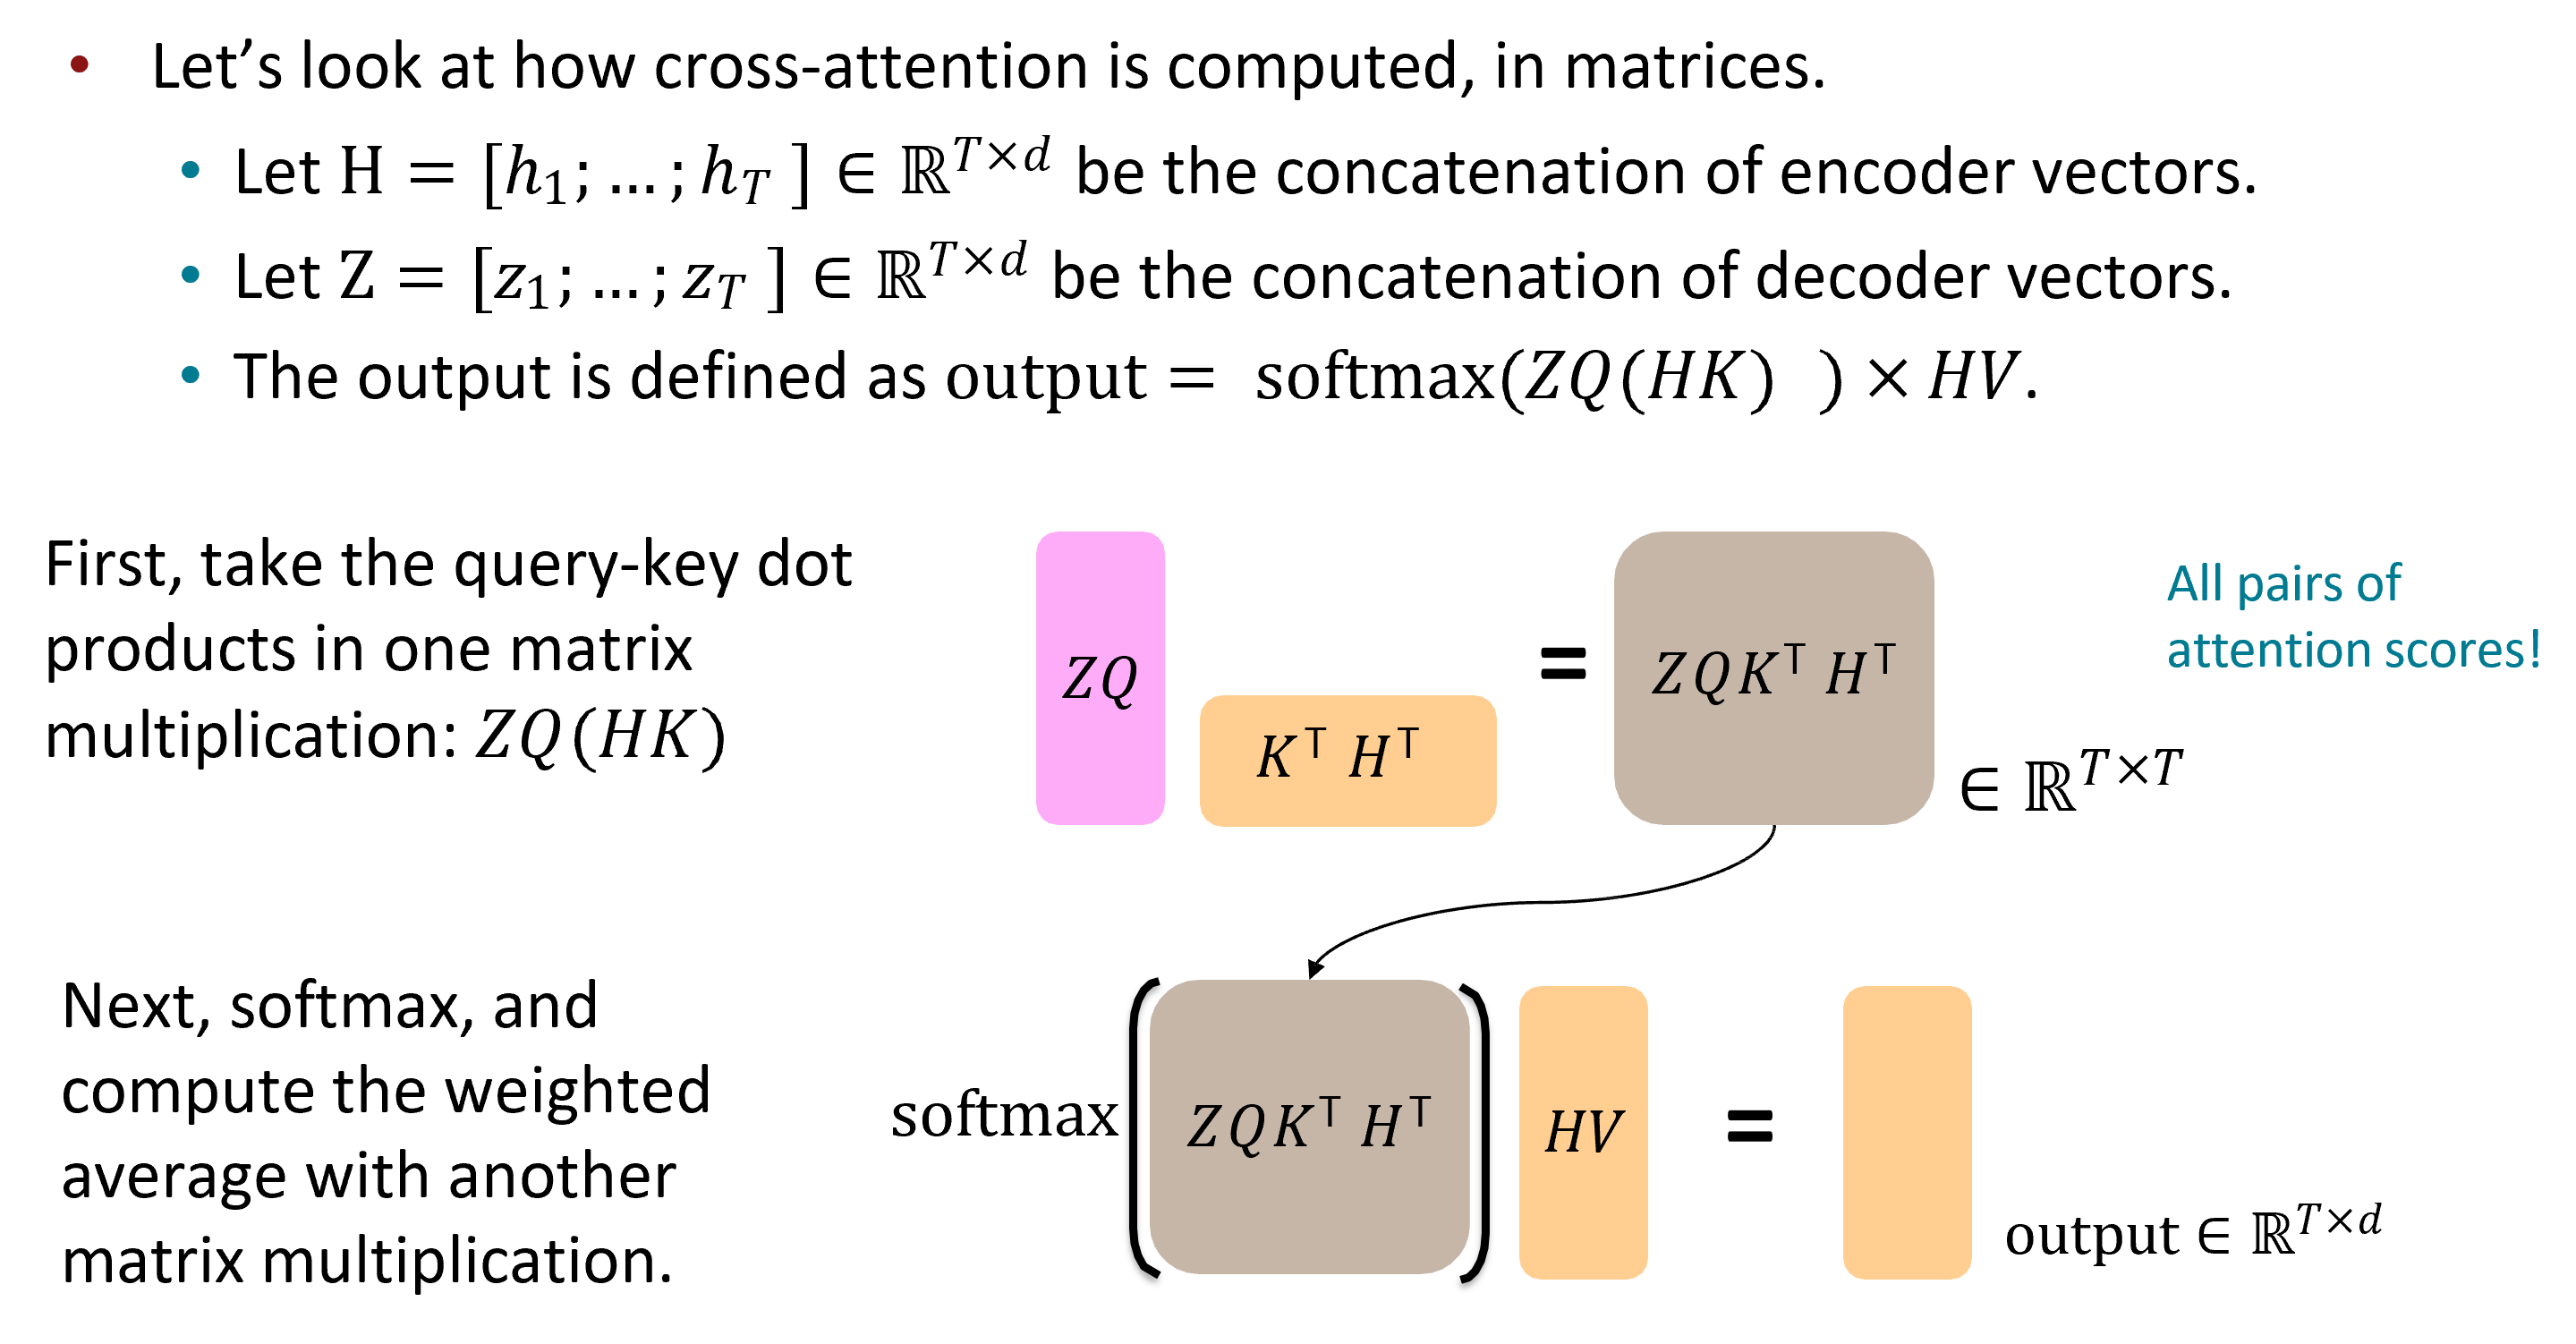
\includegraphics[width=\linewidth,keepaspectratio]{bert90}
			% \end{center}		
			
			% % {\tiny (Ref: John Hewitt)}

% \end{frame}

%%%%%%%%%%%%%%%%%%%%%%%%%%%%%%%%%%%%%%%%%%%%%%%%%%%%%%%%%%%%%%%%%%%%%%%%%%%%%%%%%%
\begin{frame}[fragile]\frametitle{}
\begin{center}
{\Large Backpropogation during training}
\end{center}
\end{frame}

%%%%%%%%%%%%%%%%%%%%%%%%%%%%%%%%%%%%%%%%%%%%%%%%%%%%%%%%%%%%%%%%%%%%%%%%%%%%%%%%%%
\begin{frame}[fragile]\frametitle{}
\begin{center}
{\Large Decoder only workflow}
\end{center}
\end{frame}
